
\documentclass[11pt, a4paper,oneside]{book}
%\documentclass[12pt, a4paper, oneside]{book}
% General imports:
\usepackage[utf8]{inputenc}
%\usepackage[utf8x]{inputenc} 
\usepackage[T1]{fontenc}	% For using icelandic Thorn character
\usepackage{amsmath}
\usepackage{amssymb}
\usepackage{amsfonts}		% Mathematic fonts (such Real numbers set)
\usepackage{graphicx}
\usepackage[spanish,es-tabla]{babel} 
\usepackage{textcomp}
\usepackage{gensymb}
\usepackage{siunitx}
\usepackage[toc,page]{appendix}

% Imports for images
\usepackage{caption}
\usepackage{subcaption}
\usepackage{wrapfig}

% Imports for euro symbol support
\usepackage[official]{eurosym}
\DeclareUnicodeCharacter{20AC}{\euro{}}
%\newcommand{\euro}{€}

% Other imports:
\usepackage{indentfirst} % Indent first paragraph
\usepackage[colorlinks=false,pdfborder={0 0 0}]{hyperref}
%\usepackage[nottoc,numbib]{tocbibind} % Add bibliography to table of contents
\usepackage{url}
\hypersetup{urlcolor=black, colorlinks=false}

\usepackage{multirow, array} % para las tablas
\usepackage{float} % para usar [H]

% Formatting margins of the pages:
\usepackage[top=2.3cm, bottom=2.29cm, left=1.6cm, right=1.47cm]{geometry}
%\usepackage[top=1.6cm, bottom=2.30cm, left=3cm, right=2.2cm]{geometry}

% Import for headersfig:estado_extrusora
\usepackage{fancyhdr}
\setlength{\headheight}{15pt}


\lhead{}
\chead{}
\rhead{}
\pagestyle{empty}


% Definitions of important data
\renewcommand{\author}{Santiago López Pina}
\renewcommand{\title}{SISTEMA DE ADQUISICÍÓN DE DATOS Y MODELADO PARCIAL DE SISTEMA DE EXTRUSIÓN DE FILAMENTO}
\newcommand{\department}{Departamento de Sistemas y Automática}
\newcommand{\teacher}{Víctor González Pacheco}

%% All this is used for inserting C++ code on some parts of the thesis
\usepackage{listings}
\usepackage{color}

\definecolor{dkgreen}{rgb}{0,0.6,0}
\definecolor{gray}{rgb}{0.5,0.5,0.5}
\definecolor{mauve}{rgb}{0.58,0,0.82}


% This is for writing algorithms on pseudocode (nicely)
\usepackage{algorithm}
\usepackage[noend]{algpseudocode}

% Each chapter will have its own header
%\newcommand{\headchapter}[1]{\chapter{#1}\rhead{#1}}

% Each section will have its own header
%\newcommand{\headsection}[1]{\section{#1}}\rhead{#1}}

% Change 'Chapter' to something more logical
%\renewcommand{\chaptername}{}

% Define a command for comments
\newcommand{\comment}[1]{\textbf{\color{red} #1}}


% Define commands for setting the language to be used in listings
\newcommand{\Cpp}{ \lstset{frame=single,
			language=C++,
			aboveskip=3mm,
			belowskip=3mm,
			showstringspaces=false,
			columns=flexible,
			basicstyle={\small\ttfamily},
			numbers=none,
			numberstyle=\tiny\color{gray},
			keywordstyle=\color{blue},
			commentstyle=\color{dkgreen},
			stringstyle=\color{mauve},
			breaklines=true,
			breakatwhitespace=true
			tabsize=3
	}}


\newcommand{\XML}{
	\lstset{ language=XML, 
		morekeywords={ModularRobot, name, simulationFile, gaitTableFolder, frequencyTable, frequencyTable,
		 Module, Joint, Connections, front, left, right, back, connectedTo, connector, orientation, 
		 Orientation, Roll, Pitch, Yaw, serialPort}}}

\newcommand{\Bash}{
	\lstset{language=bash, morekeywords={mkdir, ls, make, sudo, apt-get, add-apt-repository, python}}}

%Full reference of label
\newcommand{\fullref}[1]{\ref{#1} de la página \pageref{#1}}

% This is used for adding appendices:	
\usepackage[toc,page]{appendix}

% This is used for tables spanning more than one page:
\usepackage{longtable}
	
% This is for units not appebaring as italics
\usepackage{siunitx}
		
% This is for including pdf files
\usepackage{pdfpages}

% Enable hyphenation
\usepackage{hyphenat}

% Include PDF files
\usepackage{pdfpages}
% Include epigraph
\usepackage{epigraph}
% Evitar lineas viudas y huerfanas
% http://ocw.um.es/gat/contenidos/ldaniel/ipu_docs/latex/tema6.html
\clubpenalty=10000
\widowpenalty=10000

\renewcommand{\appendixname}{Apéndices}
\renewcommand{\appendixtocname}{Apéndices}
\renewcommand{\appendixpagename}{Apéndices}
%%%% BEGIN DOCUMENT %%%%%%%%%%%%%%%%%%%%%%%%%%%%%%%%%%%%%%%%%%%%%%%%%%%%%%%%%%%%%%%%
\begin{document}

	%%%%%%% FRONTPAGE 
	%%%%%%%%%%%%%%%%%
	\begin{center}
	
\includegraphics[width=0.25\textwidth]{./images/Logo.jpg}\\[2cm]
	\textsc{\LARGE Universidad Carlos III de Madrid}\\[0.5cm]
	\textsc{\LARGE \department}\\[0.5cm]
	\textsc{Grado en Ingeniería Electrónica, Industrial y Automática}\\[3cm]
	\textsc{\huge Trabajo final de grado}\\[1cm]
	\textsc{\LARGE \title}\\[6cm]
	\begin{table}[!ht]
	\centering
		\begin{tabular}{l l}
			Alumno: & \author \\
			Tutor: & \teacher\\
		\end{tabular}
	\end{table}

\end{center}
%====================================%
	\thispagestyle{empty}
	~
	\newpage
	\thispagestyle{empty}
	\thispagestyle{empty}

\vspace*{\fill}
	\epigraph{¿Carretera? A donde vamos no necesitamos carreteras.}{Dr. Emmett Lathrop Brown}
\vspace*{\fill}

	~
	\newpage
	\thispagestyle{empty}
	\newpage{}
\thispagestyle{empty}
\begin{center}
    \Large
    \vspace{0.9cm}
    \textbf{Agradecimientos}
\end{center}

Con este proyecto finalizo un camino que en su día no pensé poder realizar. Desde el inicio no ha sido un camino fácil, muchas han sido las veces en las que me he planteado el abandono. Sin embargo, gracias al apoyo de mis compañeros y familiares más cercanos he podido llegar a la meta final.\\

A mi tutor Víctor González, por toda la ayuda oferecida para que este proyecto se haya realizado con éxito y las charlas que hemos tenido en las tutorías, gracias.\\

A mis compañeros de clase: Mendi, Edu, Scherezade, Waaaalter, Diego y a todos los que hemos estado horas y horas durante estos cinco años en la biblioteca, ayudándonos unos a otros con dudas, tutorias conjuntas, compartiendo información valiosa y no tan valiosa, y sobre todo, compartiendo chocolate y muchas bebidas energéticas. \\

A Dani, por que desde que nos conocimos en aquella tutoria de dibujo hemos compartido muchas cosas, ayudándonos el uno al otro y haciendo práctica tras práctica. Porque con una mirada ya nos decimos mil cosas. Gracias.\\

A Obijuan, por su trabajo y dedicación por el patrimonio tecnológico de la humanidad, haciendo que todo aquel que esté cerca de él, sienta la necesidad de aprender cosas nuevas y compartirlas con el resto.\\

A Alberto Valero, por la gran confianza depositada en mi durante estos años y sin su ayuda este proyecto no estaría siendo presentado.\\

A Jose Emilio, por contar conmigo para la realización del proyecto y todo la ayuda ofrecida para poder terminar con éxito el proyecto a pesar de los problemas tenidos. Gracias por todo lo que me has enseñado en tan poco tiempo.\\

Amis compañeros de Rivas por ayudarme, todos han aportado su granito de arena en la realización del proyecto.\\

A Jorge García, por confiar más en mi de lo que yo lo hago. Gracias por convencerme de que podría empezar, y terminar, una carrera. Gracias por estar siempre que te he necesitado.\\

A Helia, por estar en esta etapa de mi vida que ha sido más complicada de lo esperado y aún así has estado a mi lado en todo momento. Gracias por la paciencia que tienes conmigo y corregirme los innumerables fallos que cometo, y en la memoría del TFG también.\\

A mi hermana y mis padres por darme todo lo que tengo y educarme para ser quien soy. No lo suelo decir a menudo, pero gracias a vosotros por confiar siempre en mi.
	~
	\newpage
	
\thispagestyle{plain}
\begin{center}
    \Large
    \vspace{0.9cm}
    \textbf{Resumen}
\end{center}

En la memoria de este trabajo fin de grado se desarrolla el proceso realizado para obtener un sistema de adquisición de datos para implementarlo en una línea de extrusión de plásticos. El sistema está compuesto de un automáta programable al cual están conectados los sensores y actuadores del sistema a controlar.\\

La totalidad del proyecto ha sido realizado en la empresa BQ el departamento de innovación y robótica, más en concreto en la reciente división de automatización y materiales.  Por tanto, este proyecto proporciona una solución a un problema real que se tiene dentro del departamento.\\

Este proyecto tendrá una continuidad temporal que no finaliza con la entrega de esta memoria y su autor, trabajará en su desarrollo.\\
\newpage{}
\begin{center}
    \Large
    \vspace{0.9cm}
    \textbf{Abstract}
\end{center}


This bachelor thesis develops the process performed to obtain a data acquisition system to implement it in a plastic extrusion line. The system consists of a programmable controller which are connected to the sensors and actuators of the control system. \\

The entire project was carried out in the company BQ in department of innovation and robotics, more specifically in the recent division of automation and materials. Therefore, this project provides a solution to a real problem that we have within the department. \\

This project will have a temporal continuity that does not end with the delivery of this report and its author, work on their development. \\
	~
	%%%%%%%Table of contents 
	%%%%%%%%%%%%%%%%%%%%%%%%
	\tableofcontents
	\newpage
	%%%%%%% Índice de Figuras y tablas
	%%%%%%%%%%%%%%%%%%%%%%%%%%%%%%%%%%
	\listoffigures   % Figures
	\listoftables    % Tables
	\newpage
	%%%%%%% Adding some header text on top of the page
	%%%%%%%%%%%%%%%%%%%%%%%%%%%%%%%%%%%%%%%%%%%%%%%%%%
	\fancyhead[L]{\nouppercase{\leftmark}}
	\fancyhead[RO]{\nouppercase{\rightmark}}
	\fancyhead[R]{}
	\fancyhead[LO]{}
	\pagestyle{fancy}
	%%%%%% Secciones del documento
	%%%%%%%%%%%%%%%%%%%%%%%%%%%%%%
	\chapter{Introducción y objetivos}
\label{cap:introduccion}

En la actualidad, la empresa BQ se ha especializado en fabricar y distribuir impresoras 3D junto con sus consumibles. En 2013, se creó un departamento de Innovación y Desarrollo, encabezado por Juan Gonzalez y Alberto Valero. En ese comienzo se distribuye material relacionado con las impresoras 3D para que cualquier persona pueda hacerse una impresora 3D. Este material no es fabricado por BQ directamente, se hace la tarea distribuidor.\\

A medida que BQ adquiere experiencia en el mercado, empieza a crear una línea de investigación para desarrollar sus propias impresoras 3D, como es el caso de la impresora Witbox y la impresora Prusa Hephestos (ver figura \ref{fig:impresoras_bq}). En este casos BQ tiene un papel importante a lo largo del desarrollo del producto, desde la elección de las características finales del mismo, así como el aspecto final del packaging, es decir, BQ pasa de tener un papel de distribuidor a ser la parte principal del desarrollo del producto.\\

\begin{figure}[H]
    \centering
    \begin{subfigure}[b]{0.4\textwidth}
        \centering
        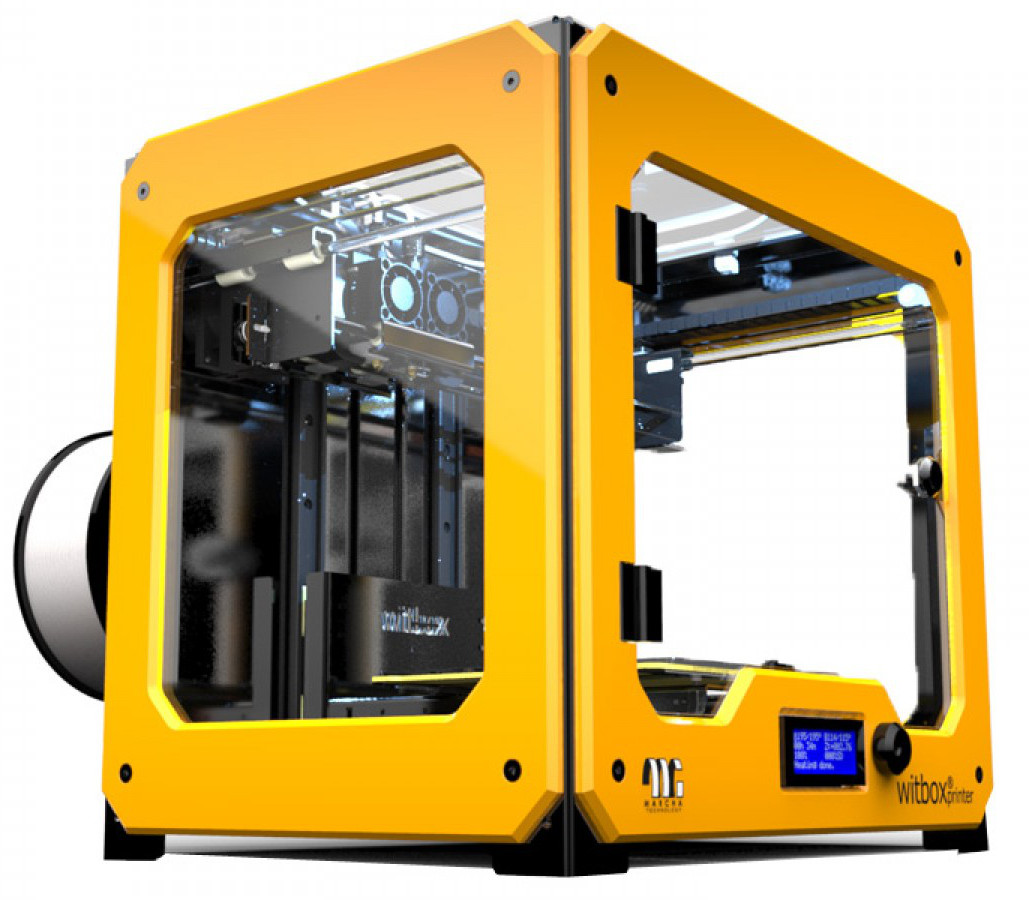
\includegraphics[width=\linewidth]{images/Witbox.jpg}
        \label{fig:estado_witbox}
    \end{subfigure}
    ~
    \begin{subfigure}[b]{0.3\textwidth}
        \centering
        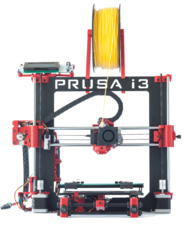
\includegraphics[width=\linewidth]{images/190px-HEPHESTOS.png}
        \label{fig:estado_hephestos}
    \end{subfigure}
    \caption[Impresoras fabricadas por BQ.]{Impresoras fabricadas por BQ. Podemos ver las dos impresoras que desarrolla BQ, a la izquierda, Witbox impresora que ya se vende montada. A la derecha, Prusa Hephestos, se vende en formato kit para que el usuario final la monte (DIY). Fuente \cite{bq}.}
    \label{fig:impresoras_bq}
\end{figure}

A la vez que se venden las impresoras 3D, BQ también vende el principal consumible para que las impresoras 3D puedan funcionar, plástico en forma de filamento. Este plástico se distribuye en unas bobinas (ver figura \ref{fig:estado_filamento}), en las que está almacenado un hilo continuo de plástico con un diámetro específico, en este caso, $1.75mm$, así mismo, cada filamento tiene un color distinto. Este consumible, es creado por otras empresas y BQ simplemente distribuye. Una vez que BQ tiene un puesto en el mercado de las impresoras 3D, decide entonces crear su propio filamento y tener más controlado la calidad del filamento que vende.\\

\begin{figure}[H]
    \centering
    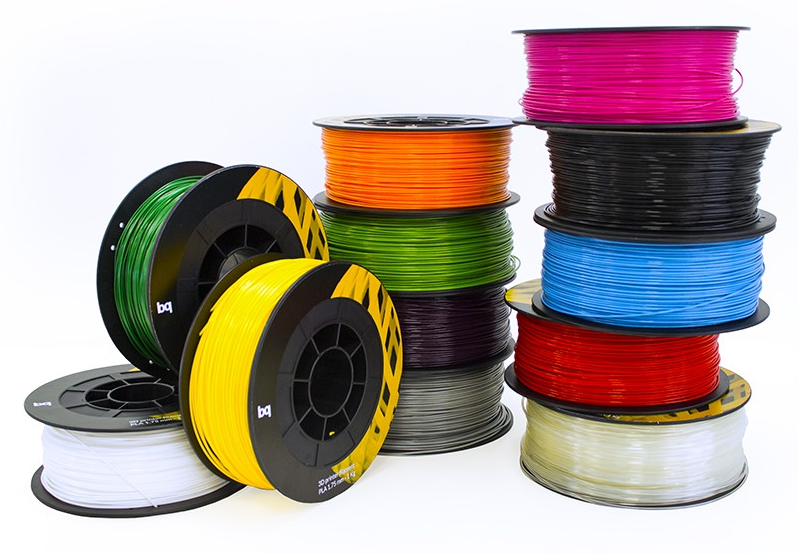
\includegraphics[width=0.5\textwidth]{images/filamento_bq.png}
    \caption[Distintos filamentos de BQ.]{Distintos filamentos de BQ. Fuente \cite{bq}}
    \label{fig:estado_filamento}
\end{figure}

Sin embargo, la fabricación del filamento es más complicada que la construcción de las impresoras 3D. Se necesitan máquinas capaces de fundir plástico y darle la forma de filamento, estás máquinas son las extrusoras, de las cuales BQ no dispone ninguna y no se tiene previsión de que al comprar una se pueda llegar a amortizar su compra. Por ello, se decide sub-contratar el proceso de fabricación a una empresa experta en la extrusión de plásticos.\\

En la provincia de Huesca, se encuentra la empresa PESL, la cual es especialista en extrusión de perfilería de plástico. BQ y PESL empiezan a trabajar en la fabricación de un filamento que cumpla las características necesarias para las impresoras 3D. En una primera aproximación estas características son, el material y el diámetro final. Después de pruebas de fabricación del filamento por parte de ambas empresas, BQ empieza a vender filamento propio.\\

Aparte de vender el filamento que fabrica PESL, BQ también lo usa para su uso en sus instalaciones y desarrollo de proyectos, se empieza a detectar entonces un problema, no todas las bobinas del mismo lote de fabricación tienen la misma calidad, llegando a darse el caso que en una misma bobina, no todo el filamento es igual. Los problemas detectados tienen que ver con el aspecto visual del filamento, la mezcla de color no es homogénea, y hace que las piezas impresas tenga un degradado. Así mismo, y mucho más importante, el diámetro del filamento no es constante (ver figura \ref{fig:muestra_filamento}).

\begin{figure}[H]
    \centering
    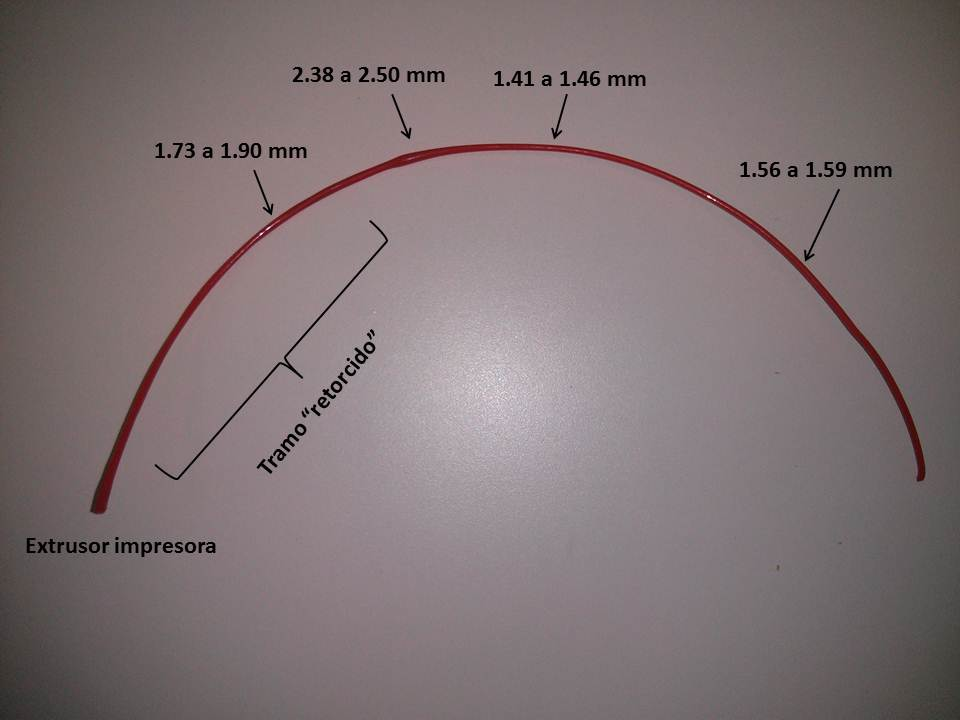
\includegraphics[width=0.6\textwidth]{images/atasco_rojo.jpg}
    \caption[Muestra de filamento con problemas en el diámetro]{Muestra de filamento con problemas en el diámetro. Podemos observar cómo en un tramo de filamento, el diámetro no es constante.}
    \label{fig:muestra_filamento}
\end{figure}

El problema que se tiene en el color, es algo secundario, ya que puede considerarse visual y no afecta a ninguno de los componentes de la impresora. No pasa lo mismo con el problema del diámetro, ya que la manera en la que se descubre, es que las impresoras dejan de imprimir pasado un tiempo, puesto que si el diámetro nominal del filamento sale de un determinado rango de valores, tanto por exceso como por déficit, se producen atascos en la impresora. Estos atascos, en el mejor de los casos, sólo supone la limpieza del extrusor de la impresora y se puede volver a utilizar, pero en ocasiones el atasco puede deja inservible el extrusor y es necesario reemplazarlo.\\

No tardan en llegar las primera reclamaciones de clientes finales, en las que su impresora deja de imprimir de forma temporal o incluso que el uso del filamento de BQ daña las impresoras 3D de los clientes, suponiendo un gasto extra para BQ, ya que ofrece una garantía por su producto y para PESL, que no todo el filamento que fabrica reporta beneficios. Es por ello que se pone en aviso a PESL y se toman decisiones para mejorar este problema.\\

A pesar de que PESL es especialista en extrusión de perfilería de plástico, es la primera vez que se dedican a la extrusión de filamento. Aunque de forma teórica no hay ninguna diferencia, si lo hay en el uso final que se va a dar al plástico. En el caso de un perfil extruido, su uso será rematar obras, recubrimiento aislante y tuberías. El uso final que se le va a dar al filamento de plástico va a suponer un refundido del material, proceso en el cual, influye la manera en cómo se fabricó. Igualmente el material con el que se trabaja, no es el mismo y requiere de otras condiciones de fabricación que las que se pensaba en una primera aproximación.\\ 

Se incorpora a la línea de fabricación un elemento mecánico, por el cual pasa el filamento, y si este supera un diámetro se parte y se deja de producir. También se empieza a registrar el diámetro del filamento y las temperaturas de fabricación en un ordenador para intentar tener un mejor control de la trazabilidad de las bobinas, y así acotar el problema que haya en la fabricación.\\

Las reclamaciones de los clientes siguen llegando a BQ y PESL y con ellas, las pérdidas para ambos. Gracias a que cada bobina contiene un código QR en el que se incluye el número de lote de fabricación, se solicitan los registros del lote de fabricación a PESL para intentar ver posibles causas. Sin embargo, el tiempo desde que se piden hasta que son dados, es demasiado amplio. Una vez que se tiene el registro, se comprueba que faltan datos de temperaturas, puesto que estos valores son introducidos a mano ya que no están conectados con el ordenador que registra la información del diámetro. Y el muestreo de los datos no es siempre constante, por lo que hay tramos de la bobina que no se tienen.\\

Desde BQ se decide entonces tomar una solución para tener todos los registros de una manera cómoda y fiable. Se piensa en desarrollar un sistema automático en el cual estén conectados todos los elementos que componen la línea de extrusión y así poder acceder a los datos de: Fecha de fabricación, diámetro final del filamento, temperaturas de todo el proceso y velocidad de extrusión. Así mismo, esta información será almacenada en una base de datos, la cual se podrá acceder de manera remota. De esta manera, se quita carga de trabajo a PESL para que se dediquen a fabricar filamento, y desde BQ se puedan analizar los datos para ver causas de fallo.\\

A continuación, se detallan los objetivos a conseguir en el proyecto:

\begin{itemize}
    \item Realizar un sistema capaz de leer la información más importante en la fabricación del filamento
    \item Instalar en una extrusora de filamento industrial.
    \item Estudio de los datos adquiridos y desarrollo del modelo teórico de la planta.
    \item Comprobar qué regulador se amolda a nuestras necesidades.
    \item Puesta en marcha del regulador en planta y comprobar resultados.
\end{itemize}
\label{Listado_objetivos}



	%1
	\chapter{Conceptos previos}
\label{cap:conceptos}

\section{Impresoras 3D}
\label{sec:immpresoras}

En los últimos años ha tenido un gran auge las denominadas impresoras 3D. Máquinas capaces de crear un objeto físico mediante un proceso de fabricación aditiva. Este tipo de fabricación está siendo una nueva revolución, de igual manera que pasó hace unos años con la conocida web 2.0, en la que el usuario era capaz de generar contenido para la propia página. Con la fabricación aditiva, pasaremos de la fabricación 1.0 (producción de objetos físicos por grandes empresas y expertos) a la fabricación 2.0 (producción de los objetos por el usuario) \cite{additive}.\\

La fabricación aditiva es una colección de procesos que unen materiales para crear objetos físicos en 3D directamente desde un diseño en ordenador. Estos procesos, se caracterizan en que van añadiendo distintas capas que conforman el elemento final (ver Figura \ref{fig:approach_am}), que es todo lo contrario al mecanizado, en la que se conforma la pieza por eliminación de material, ya sea por arranque de viruta o por abrasión.

\begin{figure}[!ht]
    \centering
    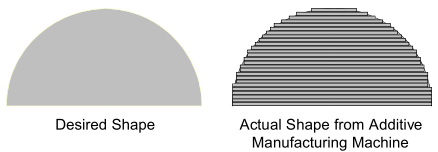
\includegraphics[width=0.6\textwidth]{images/aproximacion_am.png}
    \caption[Aproximación de una pieza con fabricación aditiva.]{Aproximación de una pieza con fabricación aditiva. A la izquierda podemos observar la forma final deseada. A la derecha la forma final obtenida y como la pieza está formada por un número determinado de capas. Fuente \cite{additive}.}
    \label{fig:approach_am}
\end{figure}

Una de las ventajas de la fabricación aditiva es su rapidez \cite{additivevssubtractive}, dependiendo de la complejidad de la pieza puede suponer un par de horas de fabricación, frente a una jornada completa de trabajo con las máquinas de mecanizado. Por ello, también se conocen a este tipo de máquinas, como máquinas de prototipado rápido.\\

Antiguamente, cuando sólo las grandes empresas disponían de ordenadores y se quería hacer algún tipo de cálculo numérico o tratamiento de información, era necesario ir a los centros de cálculos con los datos requeridos, para que, después de días o incluso semanas, obtener nuestros resultados y en el mejor de los casos, haber realizado correctamente el ensayo y no tener que volver a repetirlos, si los resultados no eran los deseados, se debería volver a repetir la operación.\\

Con la fabricación de las piezas pasa algo similar. En el caso de que quisiéramos diseñar alguna pieza para cubrir nuestras necesidades, debíamos acudir a empresas que dispusieran de las máquinas necesarias para tratar los materiales, y pasado cierto tiempo tendríamos la pieza. Una vez en nuestro poder, deberíamos comprobar que la pieza cumple con nuestras especificaciones y ver que no nos equivocáramos a la hora de tomar alguna medida y saber las tolerancias de la máquina. Gracias a la tecnología aditiva, el tiempo se ha acortado, y como veremos más adelante, a día de hoy, no es necesario acudir a ninguna empresa para poder realizar nuestras propias piezas.\\

La tecnología aditiva lleva muchos años usándose y sin embargo no ha sufrido muchos cambios desde que empresas como 3D Systems, Stratatasys o incluso el MIT, la usaran a mediados de los años 80. A pesar de ello, no ha sido hasta hace unos pocos años (2009) cuando la tecnología ha llegado al público en general. Se debe a que el funcionamiento de este tipo de tecnologías estaban protegidas por patentes. La principal patente es la que desarrolló S. Scott Crump co-fundador de Stratasys \cite{crump1992apparatus}, la cual expiro en 2009 y permitió que pudiera extenderse el uso de esta tecnología. En la Figura \ref{fig:impr_patente_sistema} podemos ver una imagen extraida de la patente.

\begin{figure}[!ht]
    \centering
    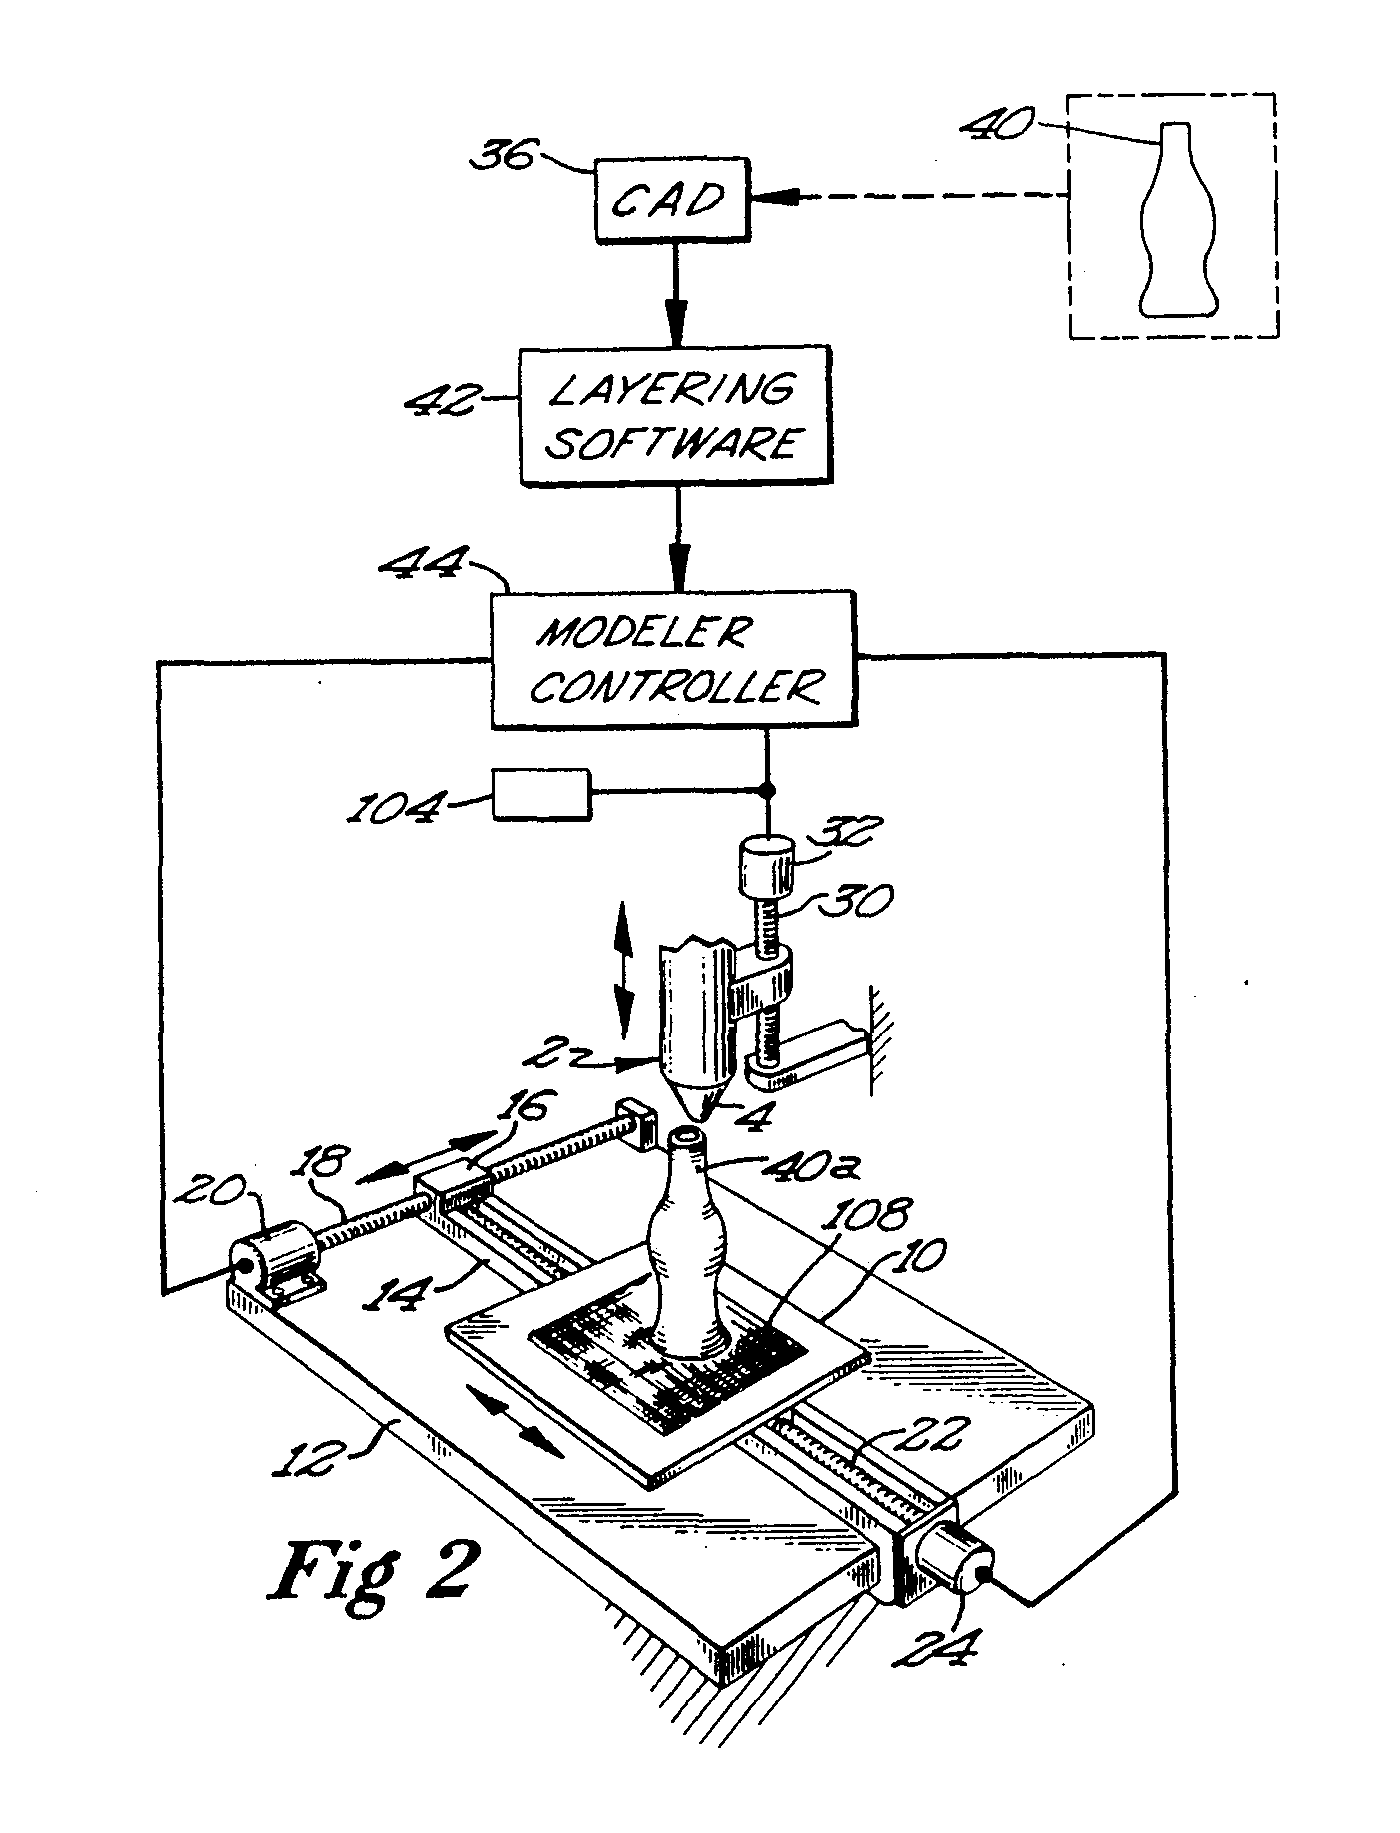
\includegraphics[width=0.6\textwidth]{images/estado.arte/US5340433-2.png}
    \caption[Esquema de la patente de S. Scott Crump.]{Esquema de la patente de S. Scott Crump en el que se detallan los distintos elementos que conforman un sistema capaz de fabricar un modelo físico a partir de un diseño generado por ordenador. Fuente  \cite{crump1992apparatus}.}
    \label{fig:impr_patente_sistema}
\end{figure}


\section{Fabricación de modelado por deposición fundido}
\label{sec:FDM}
La fabricación de modelado por deposición fundido (en inglés FDM\textregistered ) es la tecnología aditiva que más se ha popularizado en los últimos años. Aunque estas siglas están registradas por la empresa Stratasys Inc. ya que su co-fundador, S. Scott Crump fue quien desarrollo está tecnología, se usa el término equivalente, fabricación con filamento fundido (FFF).\\  

En la Figura \ref{fig:impr_fdm} podemos ver en detalle el principio de funcionamiento de este tipo de impresoras. La máquina dispone de un elemento fusor (1), que está por encima de la temperatura de transición vítrea del polímero, haciendo que entre en un estado viscoso y maleable. El fusor deposita el polímero (2) en distintos niveles sobre una superficie plana (3) a la vez que se desplaza en los tres ejes cartesianos (X,Y,Z), de este modo, la pieza es creada con el filamento que solidifica al salir del fusor.

\begin{figure}[!ht]
    \centering
    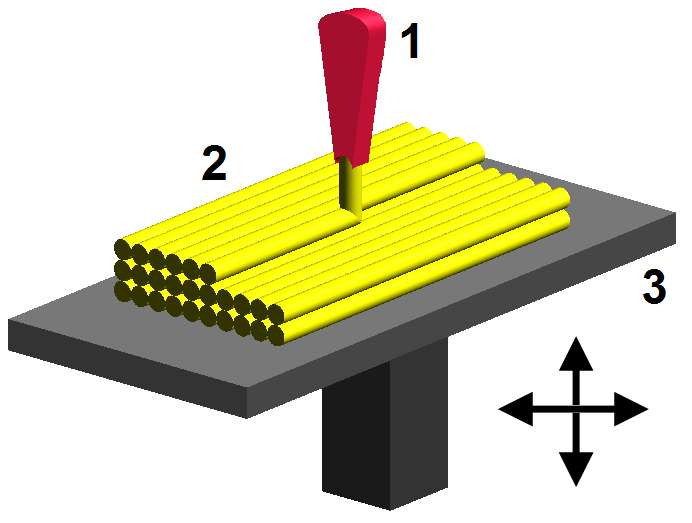
\includegraphics[width=0.4\textwidth]{images/FDM_by_Zureks.png}
    \caption[Principio de la fabricación con filamento fundido]{Principio de la fabricación con filamento fundido. (1) Elemento fusor o extrusor. (2) Polimero fundido. (3) Superficie capaz de desplazarse en los tres ejes carterianos. Fuente \cite{fundamentoFDM}.}
    \label{fig:impr_fdm}
\end{figure}

Este sistema de fabricación, tiene tres pasos definidos:

\begin{itemize}
    \item \textbf{Pre-procesado:} Un software especial lamina en capas y calcula las trayectorias necesarias para crear el objeto que queremos fabricar.
    \item \textbf{Producción:} La impresora 3D calienta el termoplástico hasta alcanzar un estado viscoso y maleable y lo va depositando en capas muy finas siguiendo las trayectorias anteriormente calculadas por el software. En los sitios en los que es necesario un soporte, el software laminador hace que se incorpore material que hará de sustento para el plástico que quede al aire, el cual será quitado de la pieza final.
    \item \textbf{Post-procesado:} Una vez que la impresora termina, la pieza será usable. En caso de haber puesto material, el usuario deberá removerlo antes de poder dar la pieza por terminada.
\end{itemize}

El modelo en 3D que se quiera construir, primero deberá ser diseñado con un programa CAD (Computer Aided Design) el cual, será exportado en un fichero con formato STL (StereoLithography). Un fichero STL es una representación triangular de una geometría en 3D. La superficie es dividida en una serie de triángulos orientados denominadas caras. Cada cara, es definida por una normal y tres puntos \cite{stl}. Sin embargo, este fichero no puede ser interpretado por una máquina FFF ya que lo único que entiende son coordenadas.\\

Por ello, el fichero STL deberá ser tratado por un programa laminador que divida el modelo 3D en distintas capas (ver Figura \ref{fig:detalle_capas}) y genere las trayectorias necesarias para realizar cada capa. Este programa, almacenará las trayectorias en un lenguaje que se denomina G-code, que es comúnmente usado en control numérico (CNC), el cuál dirá a la impresora cómo hacer la pieza deseada.

\begin{figure}[!ht]
    \centering
    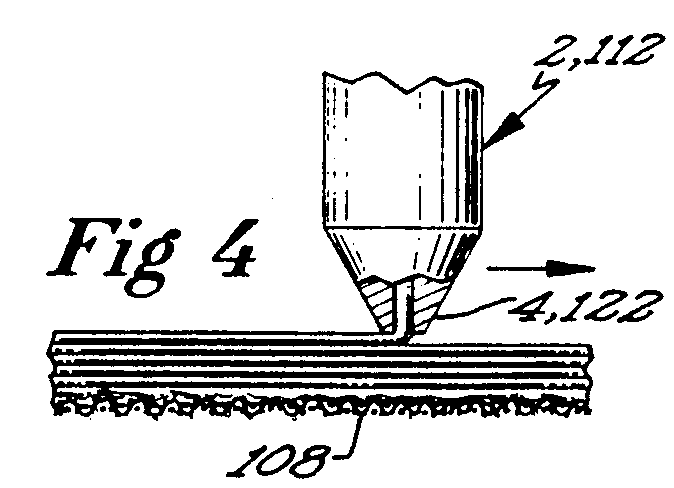
\includegraphics[width=0.4\textwidth]{images/capas_fdm.png}
    \caption[Detalle  de un extrusor realizando una pieza.]{Detalle  de un extrusor realizando una pieza.(2,112) Parte caliente por la que pasa el filamento y es fundido. (4,122) Boquilla por la que sale el filamento. (108) Distintas capas que conforman la pieza final. Fuente \cite{crump1992apparatus}.}
    \label{fig:detalle_capas}
\end{figure}

Según explica Stratasys en su página web \cite{FDMTechnology}, la tecnología FFF tiene varios beneficios que la hacen idónea para fabricar:

\begin{itemize}
    \item La tecnología es limpia y fácil de usar por el usuario.
    \item Los termoplásticos usados son estables mecánicamente y con el medio ambiente.
    \item Formas complejas que con otra tecnología serían costosas de fabricar, con FFF son mucho más practicas de realizar.
\end{itemize}

Como podemos leer en la patente de S. Scott Crump \cite{crump1992apparatus}, una impresora FDM es\footnote{Los parrafos anteriores son una traducción libre debido a que el texto original se encuentra escrito en inglés.}:

\begin{quotation}
    \emph{
    Aparato que incorpora un cabezal móvil dispensador (provisto de un suministro de material que solidifica a una temperatura predeterminada) y una base, los cuales se mueven relativamente entre sí a lo largo de los ejes “X”, “Y” y “Z” siguiendo un patrón predeterminado para crear objetos tridimensionales mediante la deposición controlada de material descargado desde el cabezal móvil sobre la base. El aparato está preferiblemente controlado por ordenador en un proceso que emplea software de diseño y fabricación asistido por ordenador (CAD-CAM) para generar señales de control y accionar el movimiento controlado del cabezal y la base mientras el material se está depositando.}\\

    \emph{La creación de objetos tridimensionales es posible mediante la deposición repetida de  capas de material de solidificación hasta alcanzar la forma deseada. Son susceptibles de uso materiales que se adhieran a la capa anterior con una unión adecuada tras la solidificación; tales como: ceras autoendurecibles, resinas termoplásticas, metales fundidos, epoxis bicomponentes,espumas y vidrios. La base de cada capa se define por la capa anterior, y el grosor de capa se define y controla mediante la altura a la que la punta del cabezal móvil está situada sobre la capa precedente}

\end{quotation}


\section{Materiales usados en impresión 3D}
\label{sec:materiales}

En la actualidad hay multitud de materiales que se pueden usar en las impresoras 3D. Siendo la mayoría de ellos polímeros termoplásticos, ya que si se les aplica una temperatura alta se vuelven deformables y al enfriarlos, pasando por un estado de transición vítrea, se endurecen.\\

Algunos materiales que se usan son:
\begin{itemize}
    \item Acrilonitrilo Butadieno Estireno o \textbf{ABS}.
    \item Poliácido Láctico o \textbf{PLA}.
    \item Alcohol de Polivinilo o \textbf{PVA} 
    \item \textbf{NYLON.}
\end{itemize}


Todos ellos tienen características que hacen idóneo su uso en diferentes campos. Por ejemplo, el ABS tiene unas propiedades mecánicas mejores que el PLA \cite{tfg_antonio}. Todos los polímeros comparten la propiedad que tienen una temperatura de fusión, relativamente baja, por lo que no es necesario un aporte de calor eleveado. Por ello, en función de la utilidad que se vaya a dar a la pieza final, será recomendable usar un polímero u otro.\\

Los materiales que han sido más utilizados dentro del mercado de las impresoras 3D, han sido ABS y PLA debido a que sus niveles de toxicidad son tolerables para el ambiente en el que van a ser tratados y las temperaturas de trabajo son relativamente bajas( en torno a $200-280 ^oC$).\\

Sin embargo, hay una característica principal que diferencía el uso de PLA frente al ABS. Durante la fabricación de la pieza con el ABS es necesario un aporte continuo de calor en la base donde se imprime mientras que el PLA no requiere de este aporte. Esto es debido a las propieades térmicas/mecánicas de los polímeros y como, en el ABS, el enfriamiento del polímero genera tensiones que hacen que la pieza se despgue de la base de impresión. Las impresoras que ofrece BQ no incluyen de serie una base que aporte calor al material. Por este motivo el plástico con el que se trabajaba es PLA.\\

Todos estos consumibles comparten la característica de como se distribuyen. El polímero es introducido en el fusor de la impresora en forma de filamento para conseguir un hilo continuo durante la impresión. Por ello, el método de fabricación del consumible es la extrusión, ya que es el método que mejor se amolda para crear objetos con una sección transversal definida y fija.

\section{Extrusión de polímeros}
\label{sec:extrusion}

La extrusión de polímeros es un proceso industrial de fabricación en el cual se hace pasar por un troquel (también denominado dado) la materia prima previamente prensada y calentada. El proceso de prensado y calentamiento, se hace en una cámara que contiene un tornillo sin fin el cual gira y es alimentado por una tolva. Al hacer pasar el polímero por el troquel, se consigue un objeto con un perfil constante y una longitud variable, pudiendo llegar a ser de centímetros, o en algunos casos de metros.\\

La Figura \ref{fig:estado_extrusora} muestrra los distintos elementos que conforman la extrusora:

\begin{figure}[!ht]
    \centering
    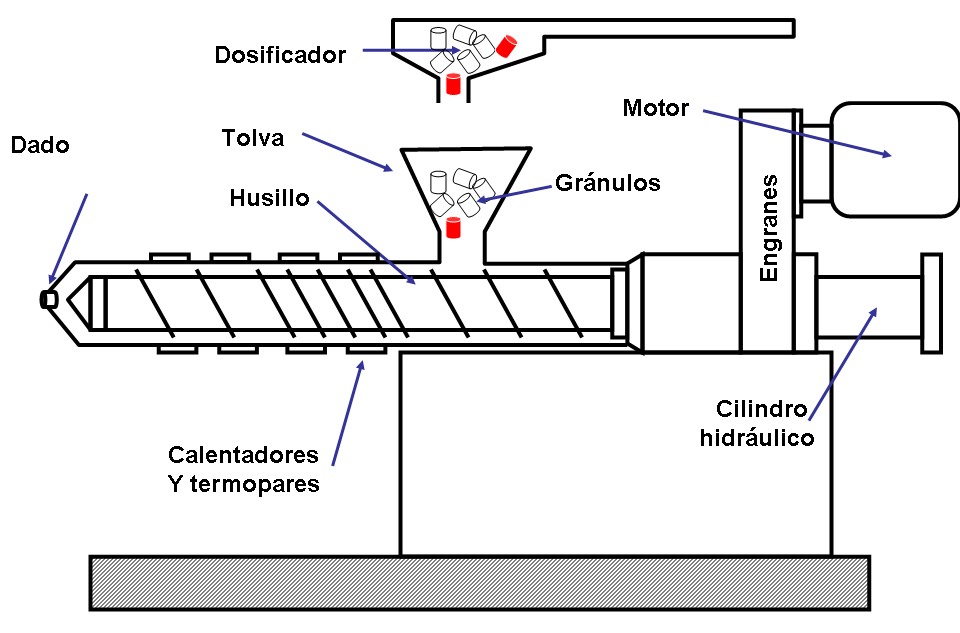
\includegraphics[width=0.6\textwidth]{images/extrusor.png}
    \caption[Esquema básico de una extrusora.]{Esquema básico de una extrusora conformado por: Dosificador, tolva, motor, husillo, calentadores y dado. Fuente \cite{disenoextrusor}.}
    \label{fig:estado_extrusora}
\end{figure}

\begin{itemize}
    \item \textbf{Dosificador:} Es el encargado de suministrar el polímero, normalmente en forma de granza(ver Figura \ref{fig:Pellets_PLA}), a la tolva garantizando un suministro constante. 
     \begin{figure}[!ht]
        \centering
        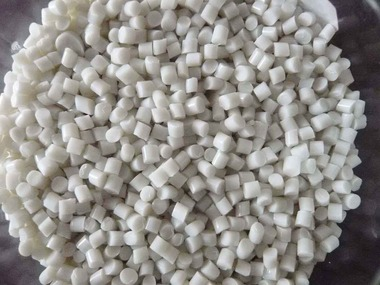
\includegraphics[width=0.4\textwidth]{images/PLA-Pellets.jpg}
        \caption[Pellets de PLA]{PLA en forma de pellets para su posterior procesado en una extrusora.}
        \label{fig:Pellets_PLA}
    \end{figure}
    \item \textbf{Tolva:} Depósito en el que cae la granza proveniente del dosificador. Debe proveer un flujo constante al extrusor para evitar cortes en el objeto que se está construyendo. Su diseño es muy importante, y en función del tipo de material que esté suministrando deberá ser de una manera u otra, debido a que el material puede llegar a compactarse en el fondo y no pasar a la extrusora. Algunos modelos de tolva incluyen sistemas de vibración para ayudar a que el material caiga. En la mayoría de los casos y dependiendo del material con el que estemos trabajando, será conveniente que incluya un sistema de secado para eliminar la humedad, puesto que dependiendo de la materia prima puede afectar a la hora de trabajar con el. Por ejemplo, con el uso del PLA es obligatorio su secado antes de la producción.
    \item \textbf{Cilindro hidráulico:} Constituye el cuerpo principal de la extrusora y en su interior está el husillo. Es en este cilindro donde se encuentran las resistencias electricas que aportan la energía calorífica necesaria para fundir el material. La temperatura está registrada a lo largo de las distintas zonas del cilindro, para poder tener un control sobre la temperatura de fusión del material. El cilindro debe estar fabricado con materiales especiales de tal manera, que tenga una buena transferencia de calor y sea más duro que el material que se está extruyendo, para lograr una larga duración.
    \item \textbf{Dado:} En función del dado que se coloque al final de la extrusora, se conseguirá un perfil distinto, en el caso que nos ocupa, el dado tiene un círculo para conseguir la forma de cilindro que deseamos.

        \begin{figure}[!ht]
                \centering
                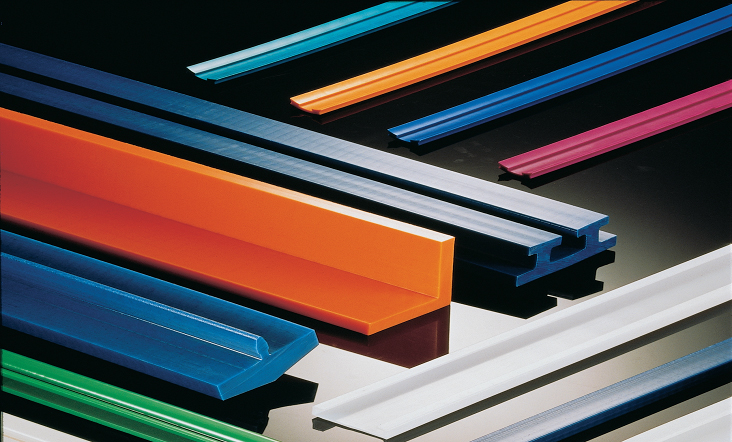
\includegraphics[width=0.5\textwidth]{images/perfiles_plastico.jpg}
                \caption[Distintos ejemplos de extrusión.]{Distintos ejemplos de extrusión con plástico. Relación de como la forma del dado influye en la forma final del material. Fuente \cite{ejemplosextrusion}.}
                \label{fig:estado_ejemplos}
        \end{figure}
    \item \textbf{Husillo:} Es el elemento más importante de la extrusora y el que determina el grado de calidad con el que la pieza saldrá de la extrusora. Como se aprecia en la Figura \ref{fig:estado_husillo} tenemos tres zonas claramente definidas:
    \begin{figure}[!ht]
            \centering
            \begin{subfigure}[b]{0.6\textwidth}
                \centering
                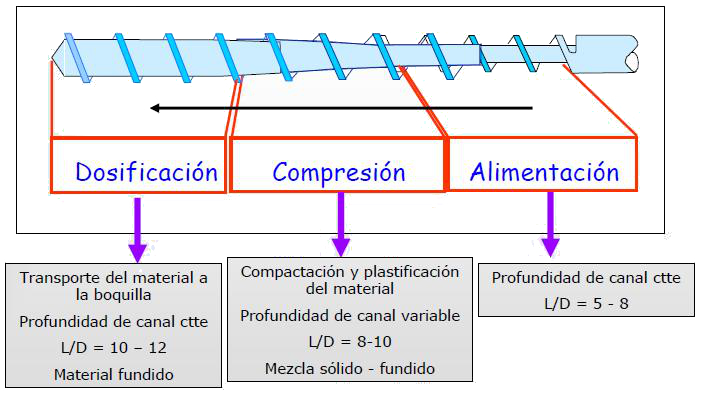
\includegraphics[width=\textwidth]{images/husillo.jpg}
                \label{fig:estado_husillo1}
            \end{subfigure}
            
            \begin{subfigure}[b]{0.7\textwidth}
                    \centering
                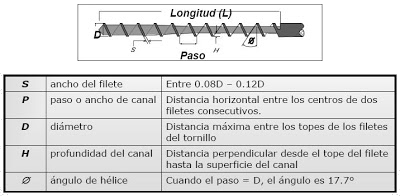
\includegraphics[width=\textwidth]{images/husillo2.jpg}
                \label{fig:estado_husillo2}
            \end{subfigure}
            \caption[Características de un husillo.]{Características de un husillo. En la imagen de la izquierda vemos las distintas zonas del husillo como son: Alimentación, compresión y dosificación. A la derecha, la relación directa que hay entre cada uno de los parámetros que definen el husillo. Fuente  \cite{parametroshusillos}.}
            \label{fig:estado_husillo}
        \end{figure}
        \begin{itemize}
                \item \textbf{Alimentación:} Esta zona, es la encargada de transportar la granza de la tolva al interior del husillo. En la Figura podemos ver como los filetes están muy separados del centro del husillo, con el fin de transportar la mayor cantidad posible de material.
                \item \textbf{Compresión:} A medida que entramos en la zona de compresión, los filetes van disminuyendo y se acercan al husillo, con el fin de fundir y homogeneizar el material. Aquí se expulsa el posible aire residual que quede entre la granza.
                \item \textbf{Dosificación:} Conduce el material compactado hacia el dado de la extrusora. Esta zona debe garantizar que el material sale con una temperatura constante y homogéneo.
        \end{itemize}
\end{itemize}

La velocidad de extrusión influye directamente en el caudal de producción de la máquina. Teóricamente, al incrementar la velocidad del husillo, obtendríamos una mayor producción en la línea, por contra repercute en la calidad final haciendo que la mezcla del producto no sea homogénea y llegando a producirse la denominada fractura del polímero fundido, que es debido a la fricción que sufre el polímero al salir por el dado. La temperatura del husillo por contra, influye en la viscosidad del polímero, este parámetro repercute directamente en la resistencia al fundido.\\

Hasta ahora, hemos visto como funciona la fabricación aditiva, y los componentes más importantes que lo forman. También la evolución a lo largo de los años de las máquinas que trabajan con esta fabricación. Ahora, vamos a ver como ha sido posible que a día de hoy, podamos tener impresoras 3D a un precio mucho más bajo y competitivo que una impresora profesional.

\section{Reprap}
El proyecto Reprap lo inicia Adrian Bowyer y su equipo en 2006 desde la Universidad de Bath \cite{jones2011reprap}. Nace con la idea de facilitar toda la información necesaria para crear y distribuir libremente una máquina de prototipado rápido (ver Figura \ref{fig:estado_darwin}).

\begin{figure}[H]
    \centering
    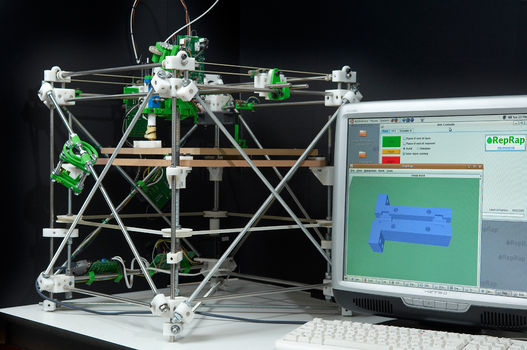
\includegraphics[width=0.6\textwidth]{images/darwin.jpg}
    \caption[Darwin,primera impresora 3D del tipo Reprap]{Darwin,primera impresora 3D del tipo Reprap. Se ve como en su construcción se usan materiales domésticos y como se hace el control desde un ordenador personal.}
    \label{fig:estado_darwin}
\end{figure}

Toda impresora Reprap, es un robot que usa fabricación con filamento fundido para hacer componentes de ingeniería y otros productos desde una variedad de polímeros termoplástico. Reprap es diseñado para que una máquina pueda ser capaz de imprimir un número importante de las piezas que contiene. El resto de piezas, serán piezas fáciles de conseguir en cualquier parte del mundo. De esta manera, se define el término autoreplicante. Toda máquina hecha dentro del proyecto Reprap será libre y open-source así, cualquiera podrá hacerse el número de máquinas que desee, ya sea desde su propia máquina Reprap, como de cualquier otra máquina.\\

Gracias a que Reprap fue liberado con una licencia libre, su expansión en los últimos años ha sido exponencial y ha facilitado que el uso de la fabricación aditiva llegue a las casas, tanto por que está disponible toda la documentación necesaria para realizar una impresora de este tipo desde su web\footnote{\url{http://www.reprap.org}}, como por la distribución a bajo costes de las máquinas.\\

A día de hoy existen más de 50 modelos distintos de impresoras 3D del tipo Reprap, a pesar de que el principio de funcionamiento es el mismo (FDM) cada impresora es distinta y tiene sus ventajas y desventajas. En contra del alto número de opciones disponibles, el modelo que más éxito ha tenido ha sido el denominado Prusa Mendel.\\

La impresora Prusa Mendel es lanzada en el año 2010 Diseñada por Josef Prusa con tan sólo 20 años, estudiante en la universidad de Praga, República Checa, y basa su diseño en la segunda impresora del proyecto Reprap, la mendel. Como se mencionó anteriormente, toda impresora liberada en Reprap es libre, por ello, Josef Prusa, tomó como base el trabajo que ya habían hecho y le añadió algunas mejoras, tales como:

\begin{itemize}
    \item Mucho más sencilla de montar.
    \item Piezas impresas más sencillas.
    \item Fácil de reparar.
    \item Usa mejores componentes lo que hacen que la calidad de impresión mejore.
\end{itemize}

Tras varios años de mejoras e iteracciones en el diseño, Josef liberó en 2012 la prusa I3. La cual introducía un nuevo diseño en la estructura, pasando de usar varillas roscadas a un marco de aluminio que sostenía todo el peso de la impresora, dándole estabilidad y robustez (ver Figura \ref{fig:evol_prusa}. Para muchas personas, fue un paso atrás en la idea originaría del proyecto Reprap ya que se intentaba conseguir que la impresora fuera capaz de imprimir al menos el 90\% de sus piezas

\begin{figure}[H]
	\centering
	\begin{subfigure}[b]{0.45\textwidth}
	    \centering
	     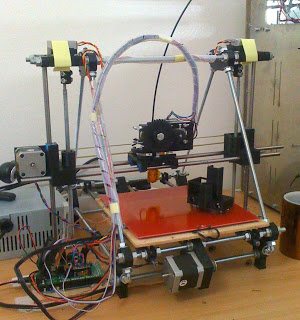
\includegraphics[width=\textwidth]{images/prusa_i2.jpg}
	    \label{fig:prusa2}
	\end{subfigure}
	~
	\begin{subfigure}[b]{0.45\textwidth}
	     \centering
	     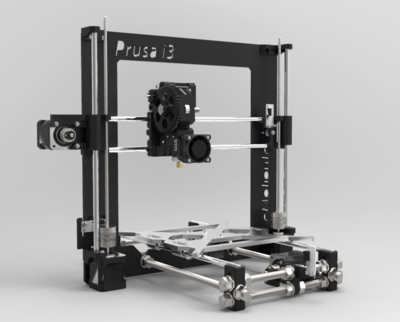
\includegraphics[width=\textwidth]{images/prusa_i3.png}
	    \label{fig:prusa3}
	\end{subfigure}
	\caption[Evolución de las impresoras diseñadas por Josef Prusa.]{En la Figura de la izquierda vemos la Prusa I2. En la Figura de la derecha la Prusa I3. Tan sólo dos años separan a ambos modelos y se ve una mejora en la simplicidad en el diseño.}
	\label{fig:evol_prusa}
\end{figure}

Pero la facilidad de montaje y que el coste por incluir un marco no incrementaba demasiado el precio final, ha hecho posible que la prusa I3 sea a día de hoy la impresora Reprap más extendida.

\section{Reprap en España}

En Febrero de 2009, Adrian Bowyer impartió una conferencia en Madrid, en el MediaLab Prado, a esa conferencia, asístió Juan Gonzalez Gomez, este era el comienzo de Reprap en España. Como el propio Juan dice en su web \cite{juan1}:

\begin{quotation}
    \emph{
    "He estado siguiendo el proyecto reprap desde hace varios años, pero sólo era una mera curiosidad. Ahora que lo he visto de cerca y he comprobado cómo son las piezas que se pueden fabricar de forma casera, estoy impactado. Estuve durante toda la charla con ese presentimiento de que estábamos al comienzo de algo grande. Es la semilla de un futuro completamente revolucionario”}
\end{quotation}

Desde ese momento, Juan empezó a investigar sobre las impresoras 3D, comprando su propia impresora 3D \cite{juanR1} y empezando a imprimir los primeros Printbot: Robots impresos en 3D, facilitando así el prototipado rápido. Debido a que la impresora que tenía no era muy fiable, pensó en la posibilidad de hacerse su propia impresora Reprap.\\

En ese momento, Juan era profesor visitante en el departamento de ingeniería de Sistemas y Automática de la \textbf{Universidad Carlos III de Madrid} junto con Alberto Valero, ambos, enseñaron a los estudiantes a trabajar con las impresoras 3D. A través de la asociación de robótica de la universidad solicitaron la compra de una impresora 3D de makerbot para que los estudiantes tuvieran acceso a una y pudieran imprimir sus propias piezas, en ese momento comenzó lo que en un futuro sería el proyecto Clone Wars\footnote{http://www.reprap.org/wiki/Proyecto\_Clone\_Wars}.\\

Juan comenzó a trabajar en la construcción de su primera impresora que fue documentando en su propio blog, para transmitírselo a los estudiantes; el 18 de Abril de 2011 se realizó la primera reunión de Clone Wars. Juan documentó todo el proceso de fabricació de una impresora Reprap en la wiki de la asociación de robótica para que de ese modo no estuviera ligado a ninguna universidad y fuera totalmente libre, más tarde toda la documentación migraría a la web oficial de Reprap.
		%2
	
\chapter{Estado del arte}
\label{cap:estado}
A la hora de tener una supervisión sobre la información producida a lo largo de un proceso productivo y poder tratarla a posteriorí, se usan sistemas software capaces de recopilar la información requerida en tiempo real del sistema y almacenarla para poder acceder a ella en un futuro.\\

Gracias a la informatización de la industria, estos sistemas están muy integrados dentro del proceso productivo puesto que, además de recopilar la información, se puede tener control directo en la producción. Una de las ventajas derivadas de la informatización, es que para tener el control del proceso, no es necesario encontrarse en el mismo lugar del mismo, gracias a Internet, se puede acceder desde cualquier parte del mundo y con cualquier dispositivo.\\

La palabra SCADA se usa para abreviar el término en inglés Supervisory Control And Data Adquisition o lo que es lo mismo, control supervisado y adquisición de datos. Un sistema SCADA puede ser utilizado en cualquer tipo de proceso en el cual se genere una cierta información que deba ser tratada por alguna persona, y se encuentre en un lugar remoto de la localización del proceso. En la Figura \ref{fig:smart_Controls} podemos observar un ejemplo de sistema SCADA orientado a la extrusión.\\

\begin{figure}[h!]
    \centering
    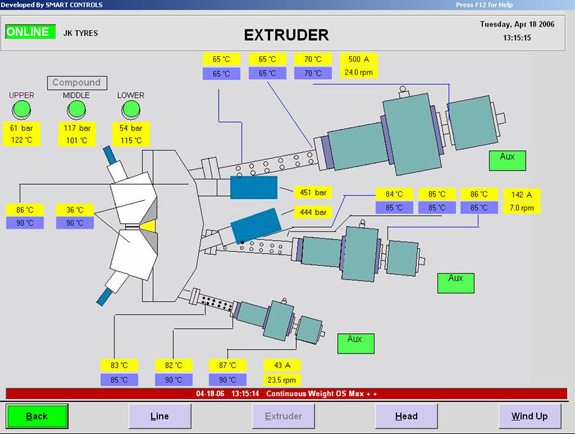
\includegraphics[width=0.6\textwidth]{images/triplex-extruder.jpg}
    \caption[Solución SCADA de la empresa SmartControls.]{Solución SCADA de la empresa SmartControls. Podemos apreciar como desde el sistema SCADA se accede a todas las variables que intervienen en el sistema. Fuente \cite{smartcontrols}.}
    \label{fig:smart_Controls}
\end{figure}

En lo referente a este tipo de aplicaciones, se han realizado avances y empresas como: Siemens, Wonderware, ABB o Rockwell Automation, ofrencen soluciones para implementar un sistema SCADA, y a día de hoy, prácticamente las soluciones son compatibles unas con otras.\\

Las distintas funciones que debe proveer un sistema SCADA son:

\begin{itemize}
    \item{Adquisición en tiempo real de los datos de intereses.}
    \item{Posibilidad de realizar gráficas de los datos adquiridos.}
    \item{Análisis de los datos obtenidos.}
    \item{Control sobre los distintos instrumentos del sistema.}
    \item{Acceso remoto al proceso productivo.}
\end{itemize}

Debido a la versatilidad de un sistema SCADA, son pocas las empresas que se dedican a una rama en concreto, se suele trabajar bajo pedido, y se diseñan sistemas SCADAS especificos para cada caso, sin embargo empresas como Castool ofrecen soluciones sistemas SCADA capaces de controlar totalmente el proceso productivo de la extrusión, Visual Optimizer \cite{castool}.\\

Castool ofrece un sistema de extrusión completo, suministrando tanto la maquinaría, software como personal cualificado para el uso de la máquina. Sin embargo esta solución solo sería útil en el caso que se adquiriera una línea de extrusión completa, en la mayoría de los casos no es lo habitual, puesto que siempre se suelen tener elementos de la linea de distintos fabricantes.\\






		%3
	\chapter{Desarrollo de la solución propuesta}
\label{cap:descrip}

Como se ha introducido a lo largo del capítulo \ref{cap:introduccion}, para el correcto funcionamiento de la línea es necesario un operador que controle y supervise el funcionamiento de la misma, realice la carga de granza en la extrusora y la carga y descarga de los carretes en la bobinadora. Debido a ello se generan errores en la producción que sólo son visibles una vez que el producto ha sido almacenado y sometido a las convenientes pruebas de calidad, almacenando asi un producto que no es de la calidad necesaria para comercializarlo.\\

Para minimizar el error humano, se propone la implementación de un sistema de aquisición y procesamiento de datos (SCADA) que permita el análisis durante y después de la producción de los diferentes parámetros del sistema. Estos son el diámetro final del filamento, las temperaturas a lo largo de la extrusora y las velocidades de extrusión. De esta manera podemos ver los aspectos que influyen en el diámetro y que el propio sistema sea capaz de corregirlo en tiempo real durante la producción. El sistema que se desarrolle, deberá ser lo más ampliable que se pueda, de esa manera, será útil en casi cualquier línea de extrusión sin importar la instrumentación que se disponga.

\section{Planificación}
\label{sec:planificacion}

El proyecto está definido por dos fases:\\

La primera fase en la que se desarrollará el sistema de adquisición de datos constará de los siguientes puntos:

\begin{itemize}
    \item Recopilación y análisis de la documentación de todos los dispositivos de interés para el proyecto de la línea de extrusión.
    \item Defición de los requisitos respecto a comunicaciones necesarias entre los dispositivos de la línea y el sistema de adquisición.
    \item Determinar los requisitos del autómata progamable industrial (PLC) a utilizar.
    \item Programación del PLC. Puesto que será el encargado de llevar el control de la planta, deberemos programar la adquisición de datos para establecer el control sobre la linea.
\end{itemize}

En esta fase se pondrá en marcha todo el sistema en la planta, instalando el PLC y cableando toda la red de comunicaciones y sensores que disponemos. Así mismo se almacenarán datos de los seis sensores de temperatura que dispone la planta (cinco de ellos en extrusora y uno en bañera de enfriamiento) y el sensor de diámetro. Con los datos adquiridos se modelará parcialmente la planta para intentar hacer un control en lazo cerrado entre la unión tractora de filamento y el sensor de diámetro del mismo. Durante esta fase se diseñará un sistema, para poder visualizar los datos adquiridos de forma remota.\\

La segunda fase del proyecto consistirá en la implementación en planta de los distintos reguladores diseñados y probados en la fase anterior. Como primera aproximación la salida a controlar será el diámetro del filamento y la entrada la velocidad de tracción, ya que es la variable que influye directamente en el diámetro a conseguir. Se estudiarán los beneficios de usar distintos tipos de controladores como pueden ser PID, fuzzy, etc. para posteriormente estudiar los beneficios e inconvenientes de cada uno de ellos.\\

Para el completo desarrollo de esta segunda fase, y poder demostrar el correcto funcionamiento en la línea, necesitaremos la aprobación de la empresa pels que explota la línea de extrusión. Aunque se tratará de un sistema modular que será fácil de integrar en otras líneas de producción parecidas. Siendo el sistema totalmente compatible y escalable para futuras lineas de extrusión que se adquieran.\\

Los plazos asignadaos a cada una de las distintas fases que componen el proyecto, se puede ver en el Anexo \ref{ane:gant}

\section{Herramientas empleadas}
\label{sec:herramientas}

\subsection{GitHub}
GitHub es una plataforma de desarrollo colaborativo en el que se pueden alojar proyectos utilizando la herramienta de control de versiones Git. El código almacenado en esta plataforma es de dominio público, sin embargo también existe la posibilidad de crear repositorios privados creándonos una cuenta de pago.\\

Para la realización del proyecto se ha creado un repositorio online \cite{githubTFG} en el que se han ido subiendo todos los ficheros que se han ido utilizando para la realización del mismo (ver Figura \ref{fig:github}).

\begin{figure}[H]
    \centering
    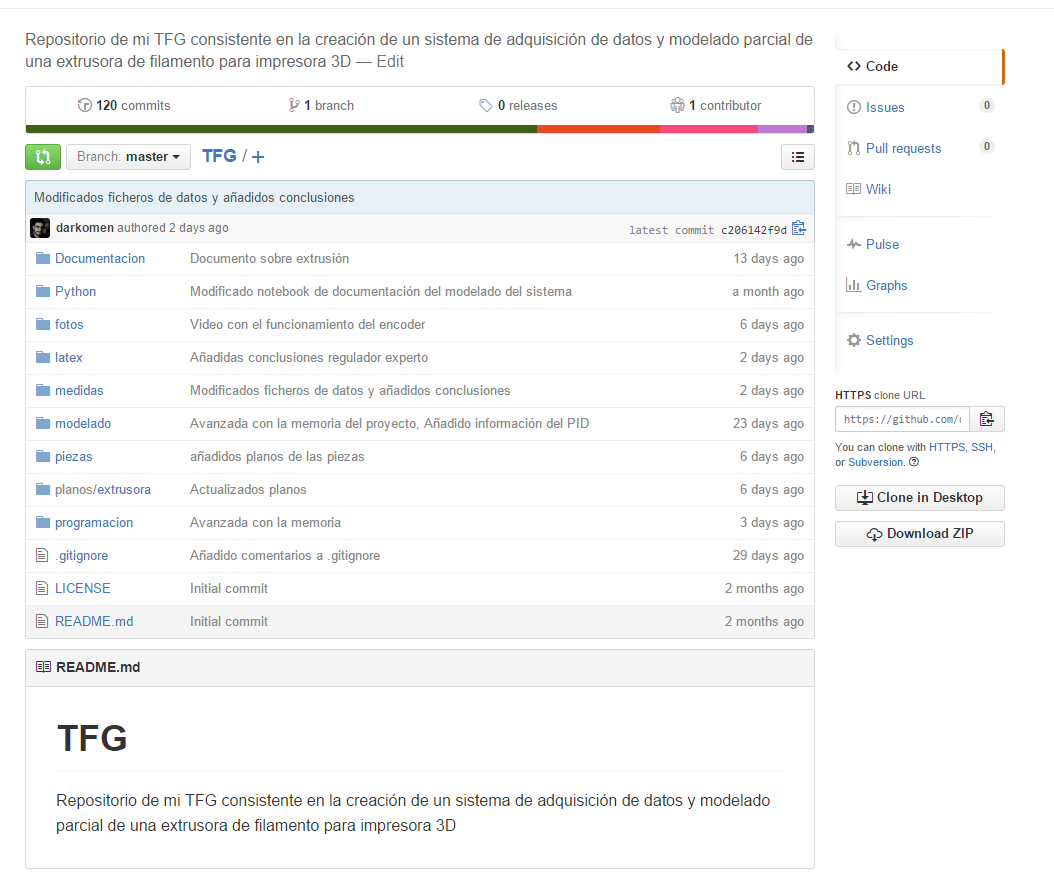
\includegraphics[width=0.65\textwidth]{images/github.png}
    \caption[Repositorio online del proyecto.]{Repositorio  en el que todos los ficheros usados para la realización del mismo están disponibles online}
    \label{fig:github}
\end{figure}

\subsection{IPython Notebook}
IPython Notebook añade funcionalidades extra a Python, como puede ser resaltado de líneas, coloreado de sintaxis, autocompletado entre otras ventajas. Además ofrece la posibilidad de combinar ejecución de código python, mostrar texto matemático, gráficas y contenido múltimedia \cite{ipython}. Podemos ver un ejemplo en la Figura \ref{fig:ipython}

\begin{figure}[H]
    \centering
    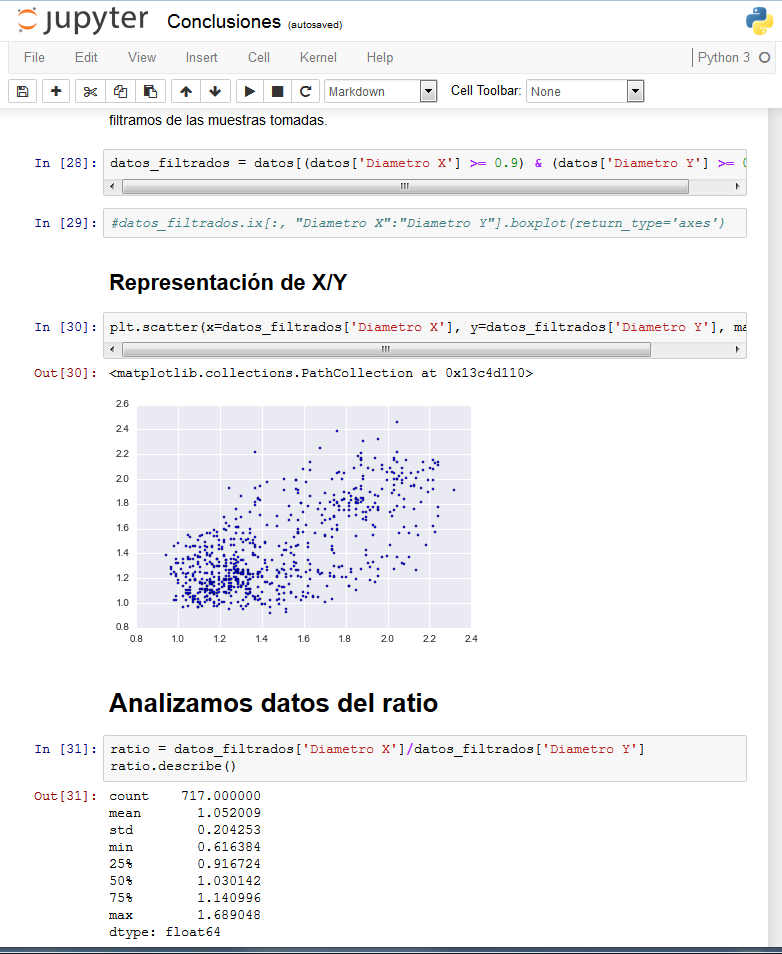
\includegraphics[width=0.5\textwidth]{images/ipython.png}
    \caption[Ejemplo de iPython Notebook usado en el proyecto.]{Ejemplo de iPython Notebook usado en el proyecto. En la Figura vemos, como se puede combinar texto plano, ejecución de código Python y mostrar gráficas}
    \label{fig:ipython}
\end{figure}

Esta herramienta se ha utilizado en el proyecto para poder calcular el modelo matemático de un sistema e implementar un regulador PID, así mismo, se han analizado los datos adquiridos durante una producción de filamento y comprobar los resultados del sistema diseñado. Los cuadernos realizados están disponibles para su consulta y descarga en el repositorio que se ha creado para el proyecto \cite{githubTFG}.

\subsection{GNU Octave}
GNU Octave es un programa libre para realizar cálculos numéricos. Ofrece un interprete de comandos, donde se van escribiendo los comandos que queramos realizar. También permite mostrar gráficas con una serie de datos numércios. Se le considera el equivalente a Matlab \cite{octave}. Esta herramienta se ha utilizado en el proyecto para calcular el modelo matemático de un sistema, para la posterior implementación de un regulador PID.

\subsection{Autodesk Inventor}
Durante la ejecución del proyecto, ha sido necesario realizar piezas específicas a nuestras necesidades. Para ello se han usado impresoras 3D y diseñado las propias piezas que en cada momento han sido necesarias. El diseño de las mismas ha sido realizado en la herramienta Autodesk Inventor. Esta herramienta ofrece un paquete de modelado de sólidos en 3D profesional que compite con otros programas de diseño asistido por ordenador, como pueden ser Catia, Pro/ENGINEER y Solid Edge entre otros.

\begin{figure}[H]
    \centering
    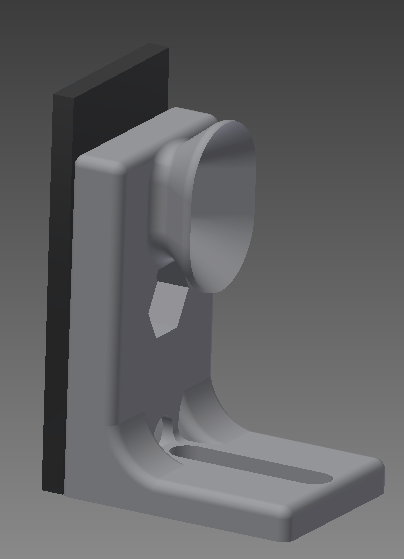
\includegraphics[width=0.25\textwidth]{images/peletizadora/guia.png}
    \caption[Ejemplo de pieza diseñada con Autodesk Inventor.]{Ejemplo de pieza diseñada con Autodesk Inventor. En la Figura vemos una pieza específica diseñada para el proyecto.}
    \label{fig:pieza}
\end{figure}

\subsection{Software de impresión 3D}
Para la fabricación de las piezas diseñadas, se han usado impresoras Witbox y un software capaz de laminar el fichero STL en G-code para que la impresión de la pieza sea correcta. En este software es donde se conFiguran los parámetros de fabricación final de la pieza.

\begin{figure}[H]
    \centering
    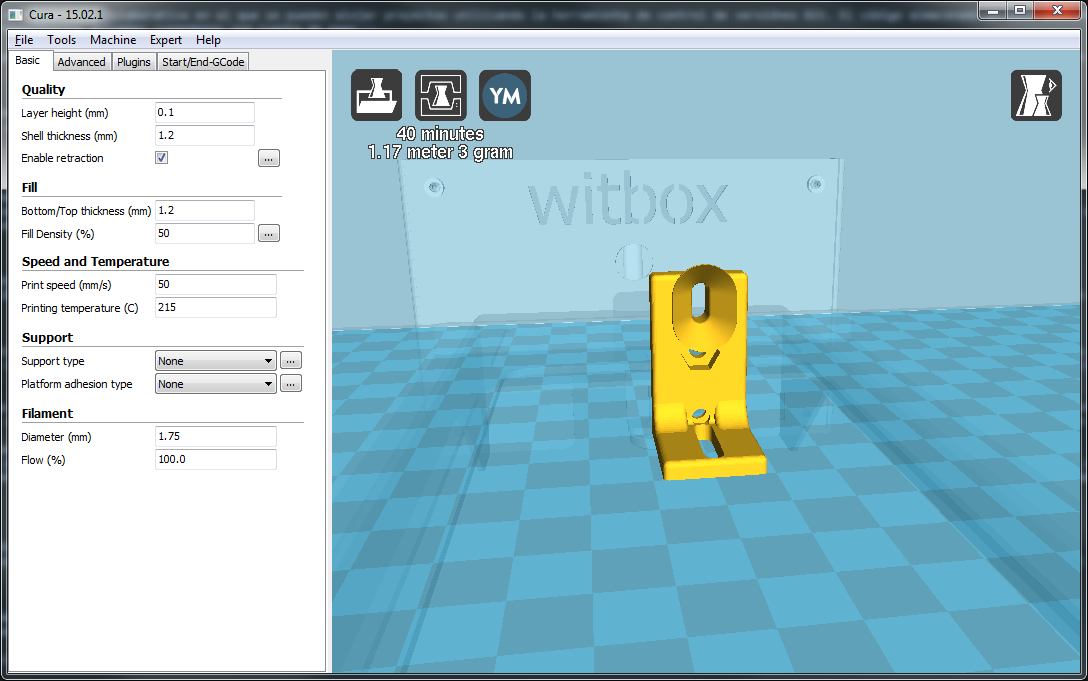
\includegraphics[width=0.7\textwidth]{images/cura.png}
    \caption[Pieza diseñada abierta en cura.]{Pieza diseñada abierta en cura. Podemos ver como en el laminador se pueden conFigurar los distintos parámetros de fabricación de la pieza.}
    \label{fig:cura}
\end{figure}


\section{Elección de los componentes.}

Se quiere desarrollar un sistema capaz de leer información de varios sensores y dado el caso activar elementos de control, todos ellos situados en un entorno industrial como es una fábrica de extrusión de polímeros. Por ello, el sistema elegido debe ser lo más robusto posible y tener capacidades de expansión por módulos para que, según la línea en la que se instale, se pueda acceder a una gran variedad de sensores.\\ 

Así mismo, el sistema debe tener la posibilidad de almacenar información en una memoria externa, ya sea, alojada dentro del mismo sistema o en un sistema externo, como puede ser un servidor de bases de datos. También, debe poder estar conectado a una red ethernet con acceso a Internet, para poder acceder de forma remota desde fuera de la fábrica.\\ 

Debido a todas estas características, se decide usar como unidad central del sistema, un autómata programable industrial (PLC) que en una primera aproximación parece ser lo más adecuado. También se intenta buscar un PLC que nos ofrezca las siguientes ventajas, no siendo estas imprescindibles, pero si ayudarán a la hora de elegir un modelo u otro:

\begin{itemize}
		\item{Licencia de desarrollo libre.}
		\item{Modelo básico con el mayor número de especificaciones necesarias.}
		\item{Capacidad de expansión de las características por medio de módulos.}
\end{itemize}

De este modo, conseguimos reducir el coste total del proyecto. Partiendo de estos requisitos y buscando distintos proveedores por Internet, las empresas que mejor se ajustan son:

\begin{itemize}
		\item{\textbf{UNITRONICS:} La compañía ofrece un PLC con pantalla HMI de bajo coste, que es idóneo para pequeños proyectos que no requieran demasiada capacidad. El principal problema es que no dispone de ninguna expansión para almacenar en tarjetas SD, ni se tiene conocimiento de que se pueda conectar a una base de datos MYSQL de forma directa.}
		\item{\textbf{WAGO:} Cumple todos los requisitos que necesitamos, sin embargo, es necesario pagar una licencia para poder usar el software disponible}
		\item{\textbf{ABB:} El PLC de la gama eco trae de serie la mayoría de las cosas que necesitamos, además, si no se superan ciertas limitaciones, no es necesario pagar una licencia para poder usar el software de desarrollo.}
\end{itemize}

Se habla con cada uno de los distribuidores que ofrecen los productos en España, pidiendo un presupuesto con el material necesario para suplir las necesidades del proyecto como vemos en la tabla \ref{tab:presupuestos}

\begin{table}[H]
	\centering
	\begin{tabular}{cc}
		{\bf Distribuidor} & {\bf Precio (\euro{})} \\ \hline
		Unitronics         & 390              \\
		Wago               & 1374             \\
		Abb                & 506              \\
	\end{tabular}
	\caption[Presupuesto de los tres distribuidores]{Presupuestos de los tres distribuidores. Se ve la gran diferencia de precios entre los distintos distribuidores.}
	\label{tab:presupuestos}
\end{table}

Debido al alto presupuesto que propone Wago se descarta ya que el precio de ABB es muy competitivo. De hecho es la marca que se elije, puesto que en comparación el coste con la marca Unitronics no supone un gasto excesivo y la fiabilidad de los autómatas y el software que provee ABB es mejor.\\

Una vez adquirido el PLC lo siguiente será realizar el montaje del armario donde irá colocado en la fábrica. En el anexo \ref{ane:plc} se detalla el proceso de construcción que se ha llevado acabo.\\

Se mantienen conversaciones con los responsables de PESL para poner en común cuales son los dispositivos que disponen en la fábrica, sin embargo, se muestran reticentes al proyecto y no nos dan acceso a su extrusora para poder realizar el proyecto.\\

A pesar de ello, no supone un problema para la realización del proyecto, ya que puede realizarse sin tener ninguno de los materiales, unicamente con el PLC y simuladores software podríamos realizarlo, pero no podríamos demostrar que nuestro sistema es útil. En el departamento de robótica e innovación de BQ se dispone de un KIT DIY de una extrusora de filamento, filastruder.\\

    \begin{figure}[H]
            \centering
            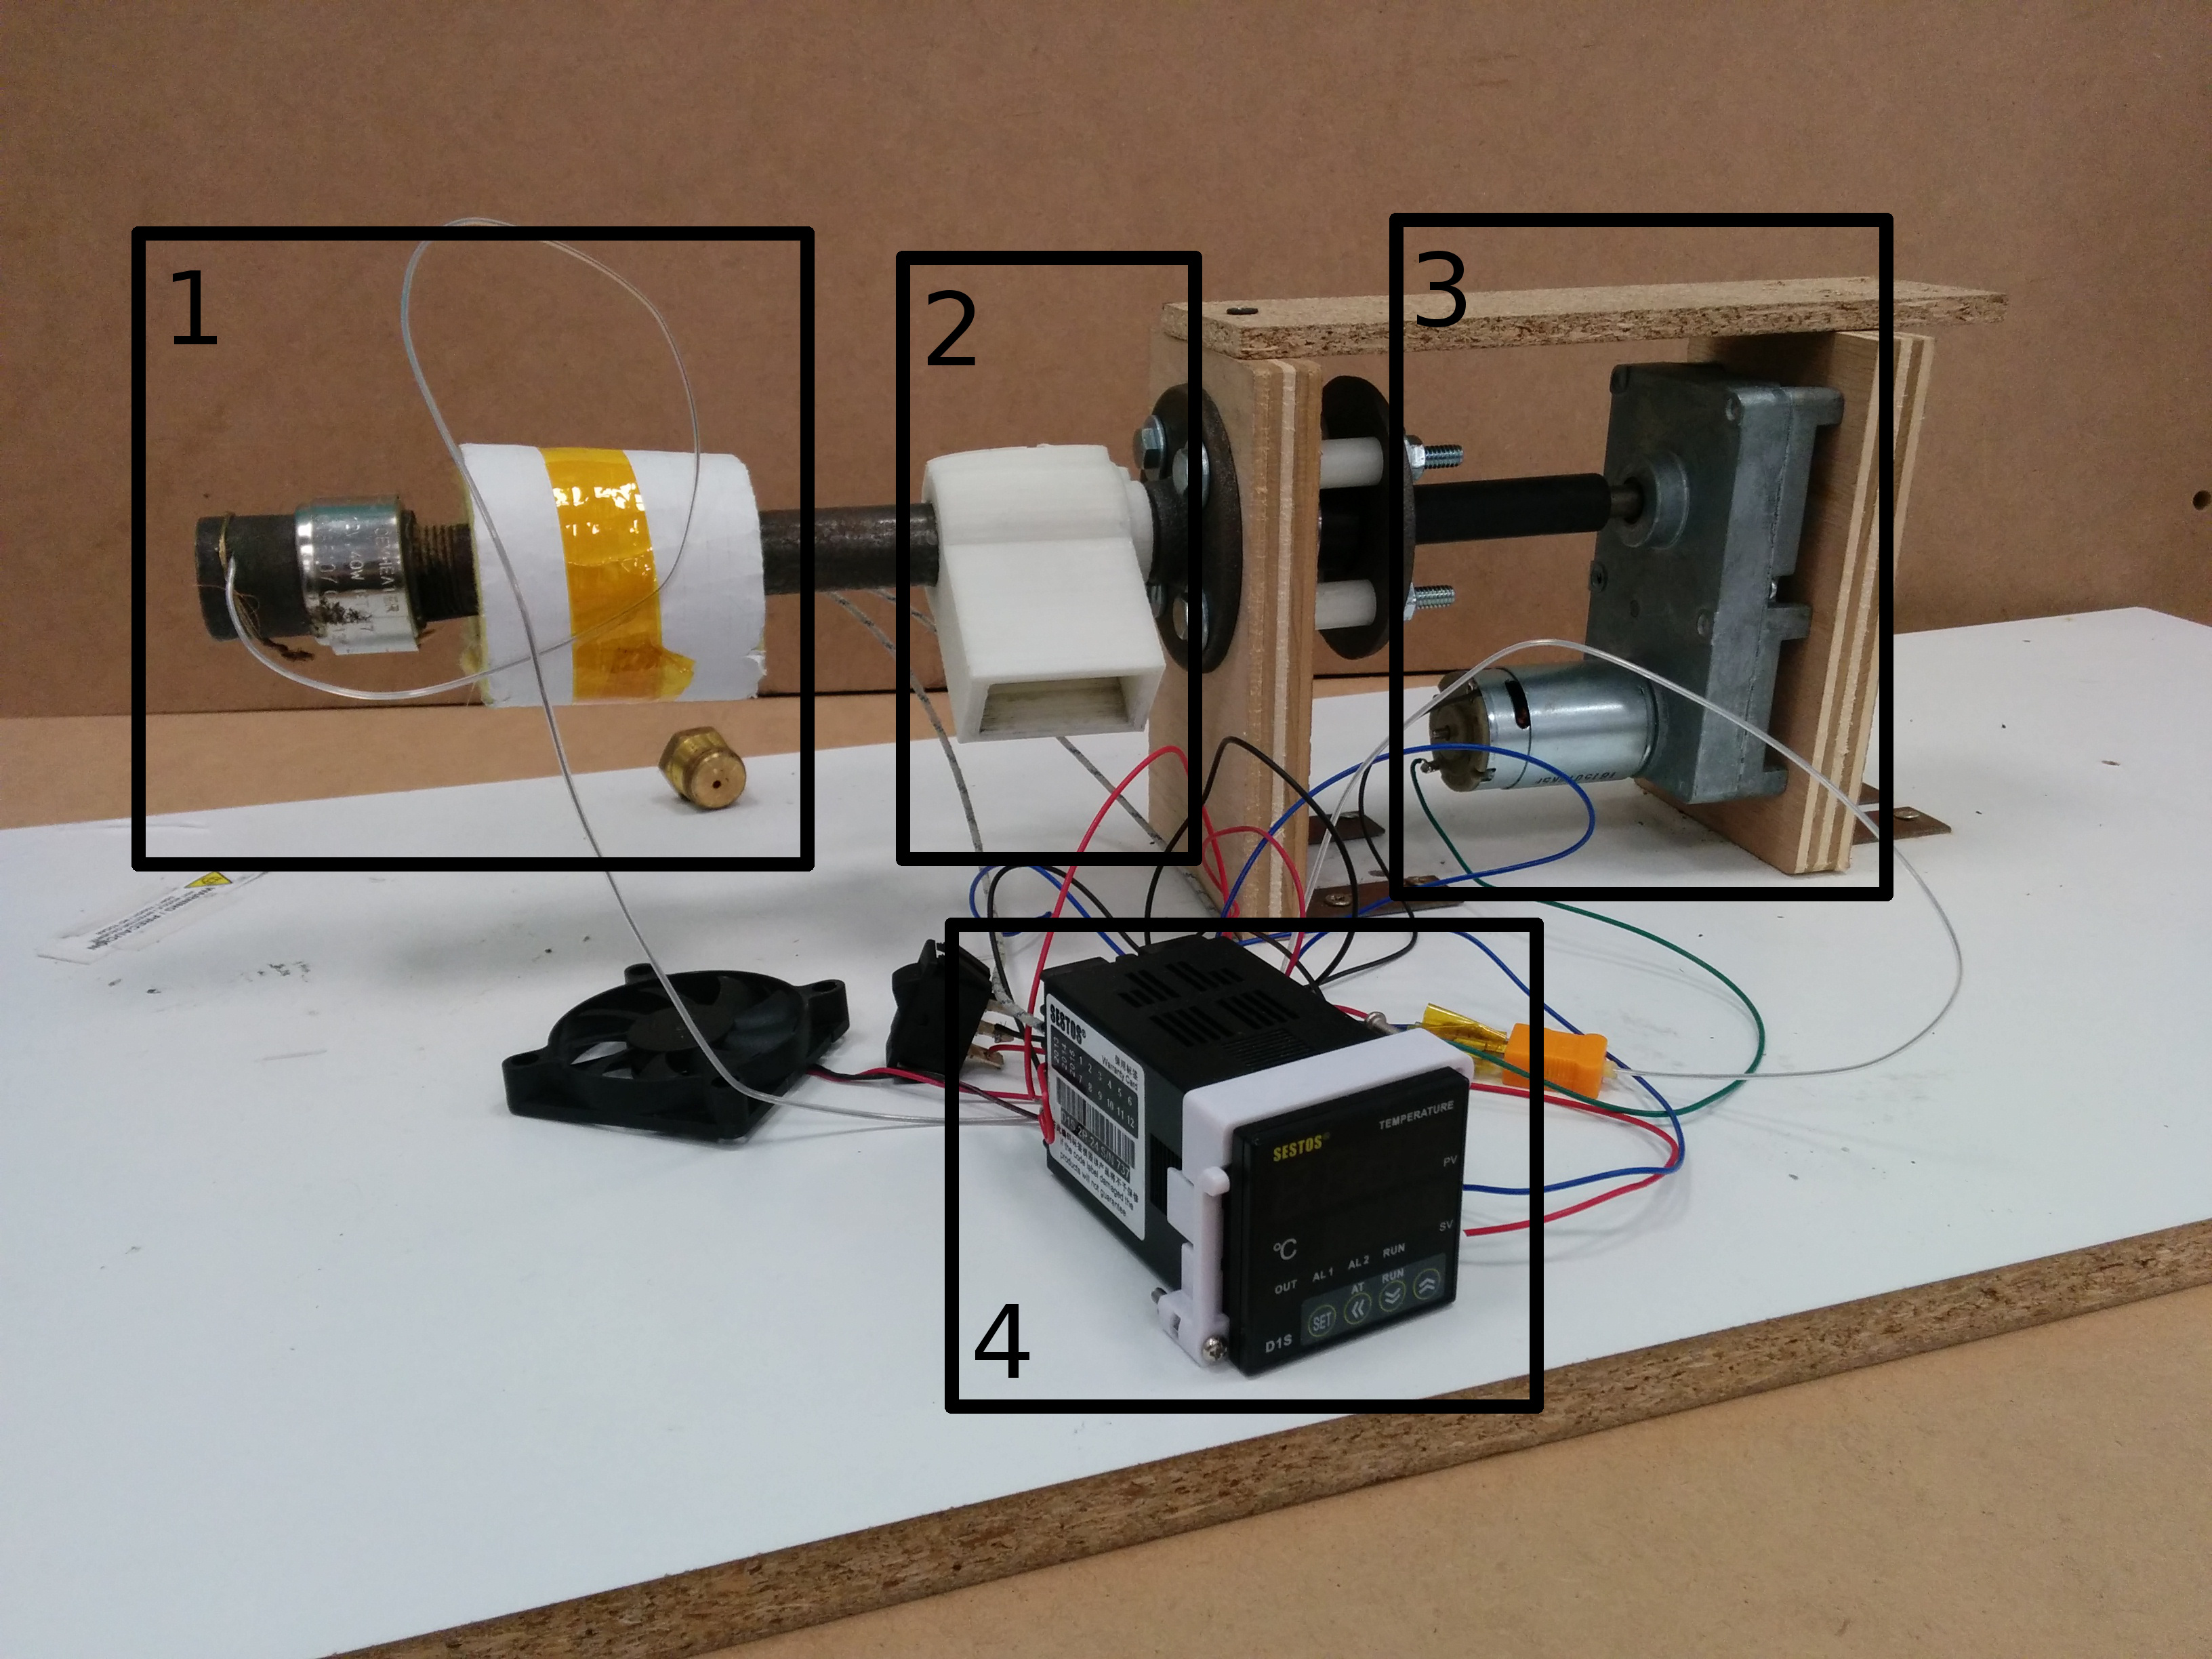
\includegraphics[width=0.6\textwidth]{images/filaextruder/IMG_20150313_11163.jpg}
            \caption[Maqueta de filastruder montada]{Maqueta de filastruder montada. (1) Boquilla y calefactor de la extrusora. (2) Tolva de alimentación de material. (3) Motor para mover el husillo. (4) Controlador de temperatura.}
            \label{fig:hardware_filastruder}
    \end{figure}

Filastruder se presenta como proyecto en Noviembre de 2012 \cite{filastruder} y consiguió recaudar $212.278 \$$ en una campaña de crowfunding en kickstarter\footnote{https://www.kickstarter.com/projects/833191773/filastruder-a-robust-inexpensive-filament-extruder?lang=es}. Es un extrusor de baja capacidad y de bajo coste, liberado como Open Source. Todo el proceso de construcción del extrusor se documentó en el foro y se creó una comunidad de usuarios interesados en los extrusores caseros.\\

Algunas de las características de este extrusor son:

\begin{table}[H]
    \centering

        \begin{tabular}{lc}
        \textbf{Par de detenimiento del motor}            & $12N.m$                           \\
        \textbf{Velocidad del motor}                      & $3 rpm$                           \\
        \textbf{Tiempo para extruir 1kg}                  & $24H$                             \\
        \textbf{Diámetro del husillo}                     & $15.875mm$                        \\
        \textbf{Longitud del husillo}                     & $255mm$                           \\
        \textbf{Tolerancia declarada}                     & $\pm 0.05 mm$                     \\    

    \end{tabular}
    \caption[Características filastruder.]{Características filastruder. Fuente\cite{tfg_diego}}
    \label{tab:caract_filas}
\end{table}

Debido a que la maqueta ha estado almacenada durante años sin usar, el funcionamientor no es el adecuado para crear filamento en condiciones, sin embargo, es completamente útil para la realización del proyecto. Ya que con dos sensores de temperatura, dos cartuchos calefactores y un sensor de diámetro, podremos simular una extrusora industrial, de esta manera también, demostramos que el sistema es totalmente escalable y con cambios en el software podremos adquirir datos de cualquier extrusora. En el anexo \ref{ane:filastruder} se detalla el proceso llevado a cabo para montar la filastruder. \\

Se decide usar un sensor de diámetro opensource del cual, toda la información necesaria para su construcción está accesible via online \cite{thing_filamento}. En el anexo \ref{ane:sensor} se detalla el proceso llevado a cabo para su construcción.\\

A la hora de obtener matería prima para poder extruir filamento, se decide construir una peletizadora para poder reciclar filamento que no cumple las condiciones para ser usado en una impresora 3D (ver anexo \ref{ane:peletizadora}). Antes de extruir el filamento, se comprueba si los pellets reciclados son aptos para la extrusión.\\

Se realizan ensayos por calorimetría diferencial de barrido (DSC). El DSC es una técnica que permite el estudio de las transiciones de fase en los materiales polímeros\cite{DSC1} lo que es de suma importancia a la hora de establecer sus condiciones de procesado y aplicaciones tecnológicas, ya que el tipo de fases y transiciones entre ellas determinan su comportamiento físico macroscópico.\\

Las medidas de DSC se hicieron en un calorímetro TA Instruments Q20 con sistema de enfriamiento y bajo atmósfera de nitrógeno. El aparato se calibró con Indio como sustancia de referencia ($Tm = 156.6 ^o C$, $\delta H = 28.45 J/g$). En el ensayo se sometió al polímero a una fusión a $20 ^o C/min$, seguida de una cristalización y una segunda fusión, a la velocidad de $5 ^o C/min$.\\

Se empleó el calor de fusión del PLA $100\%$ cristalino, 93 J/g. Los errores en la determinación de las temperaturas, en el cálculo de la entalpía y en el de la cristalinidad se estimaron en $\delta1 ^o C$, $\pm4 J/g$ y $\pm0.04$ respectivamente. El peso de las muestras osciló entre 6 y10 mg, y las temperaturas de transición, Tm y Tc se tomaron en el punto máximo de la curva endoterma o exoterma. La Tg se tomó a la temperatura en la que se alcanza la mitad de la diferencia de calor específico existente entre el estado amorfo vítreo y el amorfo elastómero, es decir $T_{g} = 0.5 \pm C_{p}$.\\

Se incluye a continuación los resultados obtenidos en el experimento. En la Figura \ref{fig:analisis_dsc} se observa cómo en condiciones térmicas de temperatura de transición vítrea (Tg) y temperatura de fusión, ambos filamentos son prácticamente iguales. Como vemos en la tabla \ref{tab:dsc2} no ocurre lo mismo con la cristanilidad del polímero, el cual difiere de uno a otro, por que las condiciones de fabricación no son las mismas.\\

\begin{figure}[H]
    \centering
    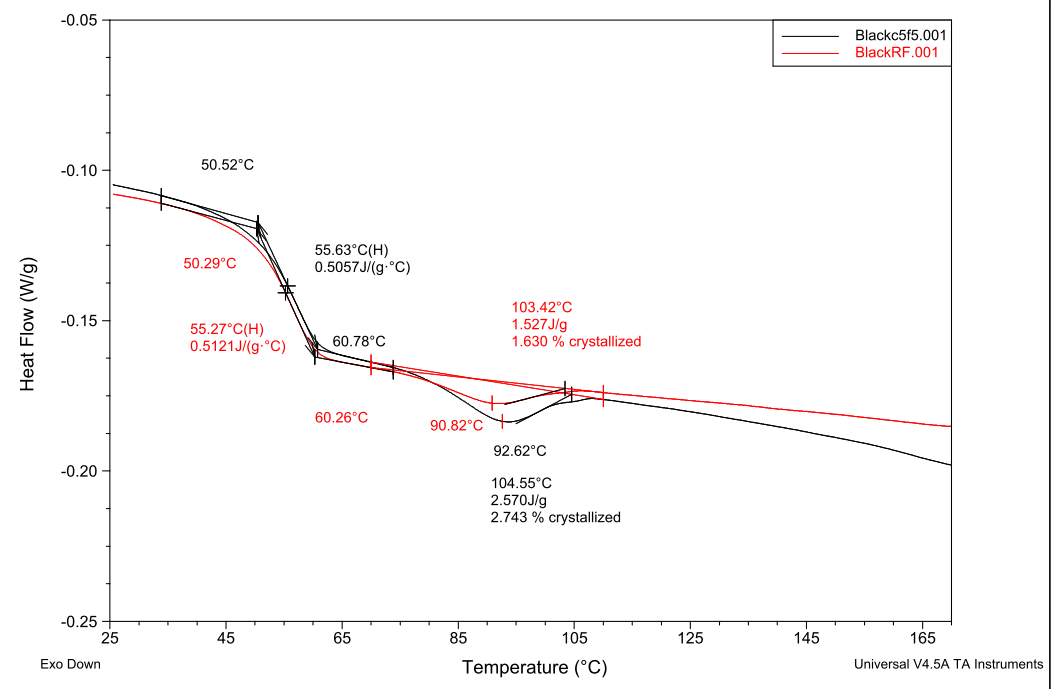
\includegraphics[width=0.9\textwidth]{images/dsc.png}
    \caption[Resultado del análisis con DSC de filamento reciclado.]{Resultado del análisis con DSC de filamento reciclado.En la imagen, vemos el filamento original (color negro) comparado coon el filamento reciclado (color rojo). Podemos llegar a la conclusión de que el filamento reciclado es apto para reutilizar.}
    \label{fig:analisis_dsc}
\end{figure}

En las tablas \ref{tab:dsc1} y \ref{tab:dsc2} podemos ver los datos obtenidos:

\begin{table}[H]
    \centering
    \begin{tabular}{llllll}
        \multicolumn{6}{c}{Glass Transition}                                                        \\
                            & Onset (ºC) & Midpoint (ºC) & End (ºC) & Height W/g & Delta Cp (J/gºC) \\ \hline
        FIlamento Inicial   & 60.78      & 55.63         & 50.52    & 0.04215    & 0.5057           \\
        Filamento reciclado & 60.26      & 55.27         & 50.29    & 0.04268    & 0.5121          
    \end{tabular}
    \caption[Datos del DSC con la transición vítrea del filamento.]{Datos del DSC con la transición vítrea del filamento. En los resultados podemos observar, cómo apenas se produce una degradación en las propiedades térmicas del material reciclado, siendo los valores, muy similares de una muestra a otra}
    \label{tab:dsc1}
\end{table} 


\begin{table}[H]
    \centering
    \begin{tabular}{lllllll}
        \multicolumn{7}{c}{Peak Integration}                                                                                 \\
                            & Start (ºC) & Onset (ºC) & Midpoint (ºC) & Stop (ºC) & Area J/g & Special Area (\% crystalized) \\ \hline
        Filamento Inicial   & 109.99     & 104.55     & 92.62         & 69.98     & 2.570    & 2.743                         \\
        Filamento reciclado & 109.99     & 103.42     & 90.82         & 69.98     & 1.527    & 1.630                        
    \end{tabular}
    \caption[Datos del DSC con la cristanilidad del filamento]{El único dato que difiere de un filamento a otro, es el porcentaje de cristanilidad, y puede ser debido a que ambos filamentos no están fabricado con la misma máquina}
    \label{tab:dsc2}
\end{table}

A falta de realizar un ensayo de propiedades mecánicas de ambos filamentos, podemos dar como válido el pellet reciclado con la peletizadora para su uso en la extrusión del mismo.

\section{Programación del PLC.}

Llegados a este punto, disponemos de todo el material necesario para la realización de una pequeña extrusora de filamento y la adquisición de sus datos más característicos en la producción. El siguiente paso es realizar la programación del PLC.\\

Las acciones que debe realizar el PLC son las siguientes:

\begin{itemize}
    \item{Controlar la temperatura del extrusor.}
    \item{Controlar motor del husillo.}
    \item{Leer información del sensor de diámetro.}
    \item{Almacenar la información tomada en un fichero de datos.}
    \item{Visualizar en una página web el estado de la producción.}
\end{itemize}

Para desarrollar el software que gestione el PLC, se usa una máquina de estados en la que pasando por diversos estados, se irán ejecutando las acciones de control. Debemos entrar en modo producción mediante la activación de una variable. Si estamos en producción, pasaremos por los distintos estados y mientras no estemos en producción, las salidas digitales y valores de consigna de los PID son reseteados a cero como medida de seguridad. Una vez que entremos en producción, el primer paso es inicializar el programa, generamos el nombre del fichero donde almacenamos los datos. Después se genera el fichero CSV y en caso de que no se produzca ningún error, se almacena la cabecera en el fichero CSV, para pasar a la producción como tal. Se controlará la temperatura del dado, se registrarán los valores de diámetros y temperaturas y se irán almacenando en el fichero CSV. El control del motor del husillo se hace de forma manual desde la visualización online.\\

La máquina de estados se muestra en la Figura \ref{fig:plc_estados}

\begin{figure}[H]
    \centering
    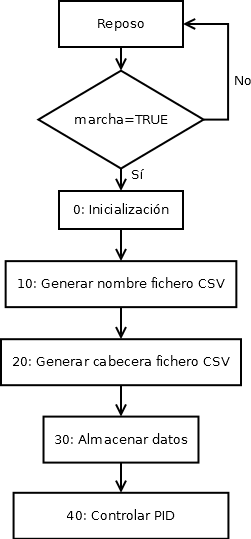
\includegraphics[width=0.25\textwidth]{images/PLC/diagrama.png}
    \caption[Diagrama de estados PLC.]{Diagrama de estados PLC.}
    \label{fig:plc_estados}
\end{figure}

\subsection{Controlar la temperatura del extrusor}
\label{sec:plc_PID}

Se implementa un regulador PID para regular la temperatura del extrusor. Es necesario conocer la planta del sistema que queremos regular para implementar de forma correcta el PID. En nuestro caso el sistema a controlar es el calentamiento del dado, por ello, debemos modelar primeramente el sistema. En la Figura \ref{fig:plc_sistema} podemos ver un esquema de un sistema con un regulador PID\\

\begin{figure}[H]
    \centering
    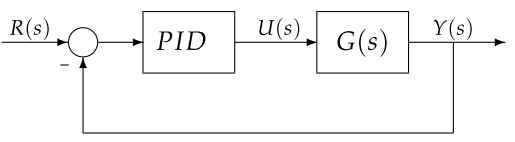
\includegraphics[width=0.4\textwidth]{images/PLC/sistema.png}
    \caption[Sistema con un regulador PID.]{Sistema con un regulador PID. La salida del sistema tendrá una realimentación a la entrada del regulador, para tomar acción de control.}
    \label{fig:plc_sistema}
\end{figure}

Con ayuda del programa que se desarrolla en el PLC haremos las siguientes tareas:

\begin{itemize}
    \item{Registrar temperaturas del dado.}
    \item{Encender de forma controlada la resistencia de calentamiento.}
    \item{Analizar los datos obtenidos.}
\end{itemize}

Analizamos como se comporta el sistema en lazo abierto, sin ningún tipo de control. Partiendo de una temperatura ambiente, se registran los valores de las temperaturas para a continuación encender la resistencia de calentamiento y ver cómo la temperatura va aumentando a medida que pasa el tiempo. Una vez que la temperatura sobrepase un valor que nosotros establezcamos, pararemos el experimento.\\

Con ayuda del lenguaje de programación Python y varias herramientas de análisis de datos como son: IPython, Scipy, Pandas y Numpy, analizamos los datos obtenidos. Las gráficas presentadas a continuación, así como los cálculos están realizadas con estas herramientas.

\begin{figure}[H]
    \centering
    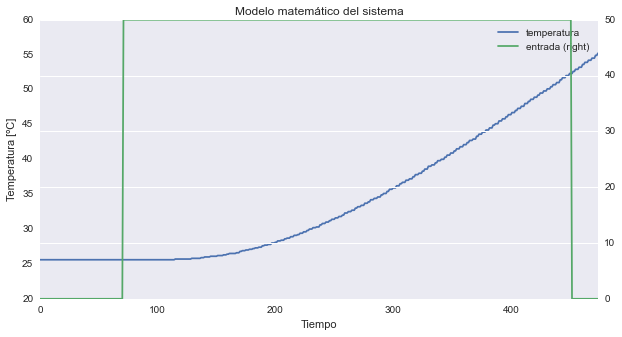
\includegraphics[width=0.75\textwidth]{images/PLC/modelado/modelado_9_1.png}
    \caption[Respuesta del sistema en lazo abierto]{Respuesta del sistema en lazo abierto. Observamos como a medida que avanza el tiempo, también lo hace la temperatura de manera exponencial.}
    \label{fig:plc_lazo_abierto}
\end{figure}

Calcularemos cual es la ecuación que mejor se ajuste a nuestros datos y tendremos el polinomio que caracteriza nuestro sistema.

\begin{figure}[H]
    \centering
    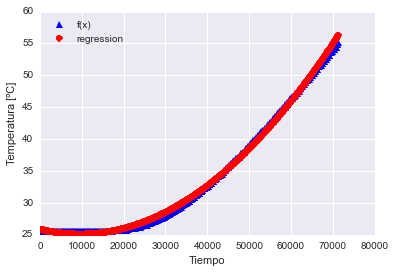
\includegraphics[width=0.5\textwidth]{images/PLC/modelado/modelado_13_1.png}
    \caption[Ajuste de la recta.]{Ajuste de la recta. Calculamos el polinomio que mejor se adapte a nuestros datos.}
    \label{fig:plc_lazo_abierto2}
\end{figure}
$$P_x=  25.9459 -1.5733 \cdot 10^{-4} \cdot X - 8.18174 \cdot 10^{-9} \cdot X^2$$

Si calculamos la transformada de laplace del sistema, obtenemos la planta de nuestro sistema, con la cual podremos implementar el regulador PID:

$$G_s = \frac{25.95 \cdot S^2 - 0.00015733 \cdot S + 1.63635 \cdot 10^{-8}}{S^3}$$

Aplicando el método de sintonizacion de Ziegler-Nichols basado en la curva reacción calcularemos el PID para poder regular correctamente el sistema.Este método consiste en estudiar el sistema en lazo abierto con escalón unitario, calculamos parámetros como la máxima pendiente de la curva y el retardo, y establecemos con ellos las ganancias del controlador PID\cite{PID}. Nos da de manera rápida unos valores de $K_p$, $K_i$ y $K_d$ orientativos, para que podamos ajustar correctamente el controlador. Con ayuda de la herramienta Open Source Octave, calculamos los valores de ganancia que serán los que apliquemos a nuestro regulador.

\Cpp
\begin{lstlisting}
pkg load control
%los datos en la funcion tf() debe ser el numerador y denominador de nuestro sistema.
H=tf([25.95 0.000157333 1.63635E-8],[1 0 0 0]);
step(H);
dt=0.150;
t=0:dt:65;
y=step(H,t);
dy=diff(y)/dt;
[m,p]=max(dy);
yi=y(p);
ti=t(p);
L=ti-yi/m
Tao=(y(end)-yi)/m+ti-L
Kp=1.2*Tao/L
Ti=2*L;
Td=0.5*L;
Ki=Kp/ti;
Kd=Kp*Td;
\end{lstlisting}

En esta primera iteración, los datos obtenidos son los siguientes: $K_p = 6082.6$ $K_i=93.868 K_d=38.9262$. Con lo que nuestro regulador tiene la siguiente ecuación característica:

$$G_s = \frac{38.9262 \cdot S^2 + 6082.6 \cdot S + 93.868}{S}$$

Una vez que tenemos las ganancias de nuestro regulador PID, volvemos a realizar el experimento de calentar la resistencia hasta un valor de temperatura deseado, en este caso 80ºC y vemos cual es la respuesta de nuestro sistema:

\begin{figure}[H]
    \centering
    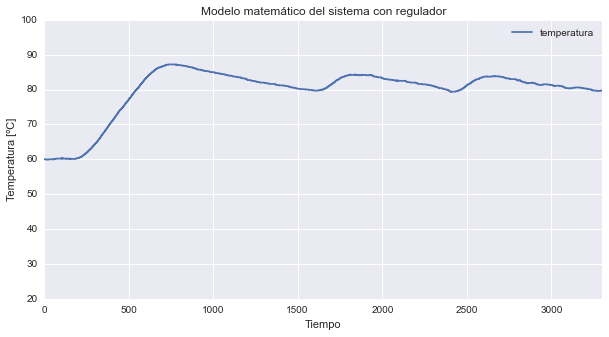
\includegraphics[width=0.75\textwidth]{images/PLC/modelado/modelado_26_1.png}
    \caption[Respuesta del sistema con PID iteracción 1.]{Respuesta del sistema con PID. Primera aproximación para obtener unos valores del regulador adecuados.}
    \label{fig:plc_PID1}
\end{figure}

Como podemos observar en la Figura \ref{fig:plc_PID1} tenemos una sobreoscilación sobre el setpoint elevada:

$$M_{p}=\frac{T_{max}-Setpoint}{Setpoint} \cdot 100 = \frac{87.20-80}{80} \cdot 100 = 9\%$$ 

Siendo el error en régimen  permanente de 3.70.\\

Una vez introducido el controlador, la temperatura tiende a estabilizarse, sin embargo tiene mucha sobreoscilación. Por ello aumentaremos los valores de $K_i$ y $K_d$, siendo los valores de esta segunda iteracción los siguientes:
$K_p = 6082.6$ ,$K_i=103.25$ y $K_d=51.425$\\

Realizando una segunda iteracción en el cálculo de nuestro regulador obtenemos lo siguiente:

\begin{figure}[H]
    \centering
    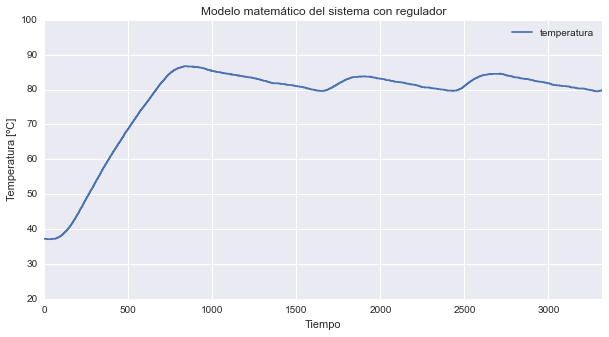
\includegraphics[width=0.75\textwidth]{images/PLC/modelado/modelado_30_1.png}
    \caption[Respuesta del sistema con PID. Iteracción 2]{Respuesta del sistema con PID. Segunda aproximación para obtener unos valores del regulador adecuados.}
    \label{fig:plc_PID2}
\end{figure}

Esta vez los resultados obtenidos son:
$$M_{p}=\frac{T_{max}-Setpoint}{Setpoint} \cdot 100 = \frac{86.70-80}{80} \cdot 100 = 8.38\%$$ 

Siendo el error en régimen permanente de 3.50.\\

En esta segunda iteracción hemos logrado bajar la sobreoscilación inicial, pero tenemos mayor error en regimen permanente. Por ello volvemos a aumentar los valores de $K_i$ y $K_d$ siendo los valores de esta tercera iteracción los siguientes: $K_p = 6082.6$, $K_i=121.64$ y $K_d=60$\\

Realizando una tercera iteracción en el cálculo de nuestro regulador obtenemos lo siguiente:

\begin{figure}[H]
    \centering
    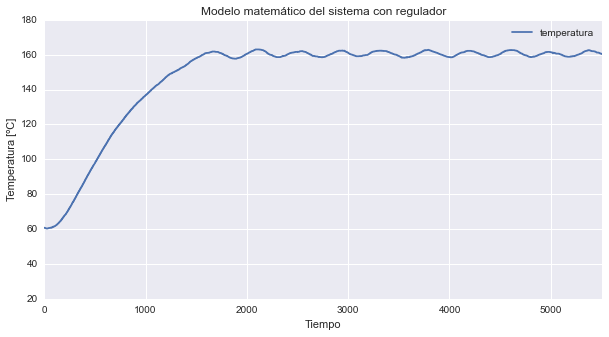
\includegraphics[width=0.75\textwidth]{images/PLC/modelado/modelado_34_1.png}
    \caption[Respuesta del sistema con PID. Iteracción 3]{Respuesta del sistema con PID. Tercera aproximación para obtener unos valores del regulador adecuados.}
    \label{fig:plc_PID3}
\end{figure}

Los resultados obtenidos son:
$$M_{p}=\frac{T_{max}-Setpoint}{Setpoint} \cdot 100 = \frac{163-160}{160} \cdot 100 = 1.88\%$$ 

Siendo el error en régimen permanente de 1.30\\

En este caso, se puso un setpoint de 160ºC. Como vemos, la sobreoscilación inicial ha disminuido en comparación con la anterior iteracción y el error en regimen permanente es menor. Para intentar minimar el error, aumentaremos únicamente el valor de $K_i$. Siendo los valores de esta cuarta iteracción del regulador los siguientes: $K_p = 6082.6$, $K_i=121.64$ y $K_d=150$\\

Realizando una cuarta iteracción en el cálculo de nuestro regulador obtenemos lo siguiente:

\begin{figure}[H]
    \centering
    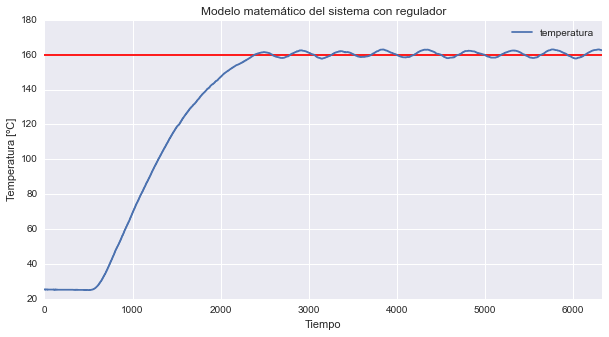
\includegraphics[width=0.75\textwidth]{images/PLC/modelado/modelado_38_1.png}
    \caption[Respuesta del sistema con PID. Iteracción 4]{Respuesta del sistema con PID. Cuarta aproximación para obtener unos valores del regulador adecuados. 4}
    \label{fig:plc_PID4}
\end{figure}

Esta vez los resultados son algo mejores:
$$M_{p}=\frac{T_{max}-Setpoint}{Setpoint} \cdot 100 = \frac{163-160}{160} \cdot 100 = 1.88\%$$ 

Siendo el error en régimen permanente de 1.10\\

Por lo tanto, el regulador que cumple con las especificaciones deseadas tiene la siguiente ecuación característica:
$$G_s = \frac{150 \cdot S^2 + 6082.6 \cdot S + 121.64}{S}$$

\subsection{Leer la información del sensor de diámetro}
\label{sec:plc_diametro}

Los sensores de diámetro están conectados a dos entradas analógicas de tensión del PLC. Será necesario unir la señal de masa (GND) del PLC con la del sensor, para que la referencia al nivel de tensión 0v sea la misma, posteriormente, la salida del sensor de diámetro, se conectará con la entrada analógica del PLC.\\

El PLC convierte el valor de tensión comprendido entre un rango de 0-10V a un valor numérico, a través de un conversor analógico a digital (ADC) de 10bits, es decir, tenemos una resolución de:

$$ \text{Resolución}=\frac{ V_{max} } {2^{10} } = \frac{10}{1024} = 9.76 mV$$

En la ayuda que ofrece el programa de ABB, se observan los valores que asigna el ADC:

\begin{table}[H]
    \centering
    \begin{tabular}{|c|c|c|}
        \hline
        {\bf Intervalo}                   & {\bf 0 ... 10V}                                                   & \multicolumn{1}{l|}{{\bf Valor digital}}                       \\ \hline
        Desbordamiento                    & \textgreater 11.7589                                              & 32767                                                         \\ \hline
        Valor de medición desmasiado alto & \begin{tabular}[c]{@{}c@{}}11.7589\\ .\\ .\\ 10.0004\end{tabular} & \begin{tabular}[c]{@{}c@{}}32511\\ .\\ .\\ 27649\end{tabular} \\ \hline
        Intervalo normal                  & \begin{tabular}[c]{@{}c@{}}10.000\\ .\\ .\\ 0.0004\end{tabular}   & \begin{tabular}[c]{@{}c@{}}27648\\ .\\ .\\ 1\end{tabular}     \\ \hline
    \end{tabular}
    \caption[Valores de conversión del ADC.]{Valores de conversión del conversor analógico a digital. Para un valor de tensión dado, se le asigna un valor decimal.}
    \label{tab:reso_adc}
\end{table}

Se va a trabajar con el rango de intervalo normal. Para poder saber el diámetro que está dando el sensor, se debe leer la entrada analógica y convertir el valor décimal a un valor de tensión, es decir, convertir el valor digital a analogico (DAC), para ello, con los valores del intervalo normal de la tabla \ref{tab:reso_adc} se calcula la ecuación de la recta que lo caracteriza que en este caso es: $Y=3.6168 \cdot 10^{-4} \cdot X$ (ver Figura \ref{fig:plc_DAC})

\begin{figure}[H]
    \centering
    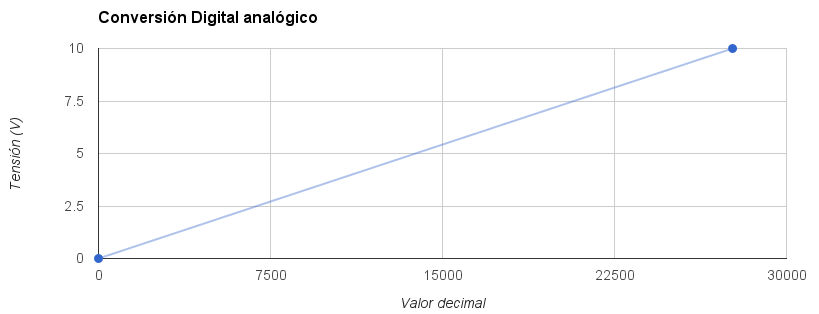
\includegraphics[width=0.75\textwidth]{images/PLC/image.png}
    \caption[Ecuación característica del ADC.]{Ecuación característica del ADC. Con esta ecuación, podemos convertir el valor de tensión a un valor de diámetro.} 
    \label{fig:plc_DAC}
\end{figure}

Con este valor se puede tener acceso al valor del diámetro que tiene el filamento. El siguiente paso entonces, será realizar el almacenamiento de los datos de la producción en un fichero para su posterior análisis.

\subsection{Almacenar la información registrada}
\label{sec:plc_SD}

Se elije un nombre de fichero en el que se usa año, mes, día y minuto para identificar la producción, es decir, tiene un formato \textit{YYMMDDmm.CSV}. El formato elegido para almacenar la información es el de valores separados por coma (CSV). El motivo por el cual se elije este formato es debido a su estandarización y que almacena los datos de forma tabular en texto plano. Gracias a esto, se puede abrir el fichero CSV con cualquier editor de texto y otros programas de hojas de cálculo, para el posterior análisis de los datos, que es uno de los objetivos del proyecto. Por lo tanto, el formato CSV es el idóneo para poder trabajar en el futuro con los datos almacenados.\\

En el progama del PLC se genera una cabecera del fichero CSV, que es la primera fila del fichero, en donde indicará la información que contiene cada columna. La información almacenada en el fichero CSV es la siguiente:

\begin{itemize}
    \item{\textbf{Time Stamp: }Es una secuencia de caracteres en las que se indican hora y fecha de un evento ocurrido. Se almacena con el formato YY-MM-DD HH:MM:SS. Con esta información podremos tener una trazabilidad del filamento almacenado y en caso de producirse un error, ver el momento concreto del mismo.}
    \item{\textbf{Temperaturas: }Valores con las temperaturas del dado y el husillo en la zona de alimentación. De esta manera se comprueba que la temperatura no sufre algún cambio drástico durante el proceso, que puede ser causante de un problema en la calidad final del filamento.}
    \item{\textbf{Diámetros: }Se almacenan los diámetros medidos por el sensor. En este caso se van a poner dos sensores de diámetro para hacer una medición en los dos ejes del filamento.}
    \item{\textbf{Información varia: }Se puede almacenar cualquier información que nosotros deseemos en un futuro (X e Y).}
\end{itemize}

En la tabla \ref{tab:plc_csv} se ve un ejemplo de los datos almacenados en un fichero csv:

\begin{table}[H]
    \centering
    \begin{tabular}{ccccc}
        {\bf time}         & {\bf Tmp Husillo} & {\bf Tmp Nozzle} & {\bf Diámetro X} & {\bf Diámetro Y} \\ \hline
        2015-8-13 11:11:1  & 67.5              & 150.4            & 1.71         & 1.49         \\
        2015-8-13 11:11:2  & 67.5              & 150.4            & 1.82         & 1.51         \\
        2015-8-13 11:11:4  & 67.5              & 150.5            & 1.91         & 1.52         \\
        2015-8-13 11:11:5  & 67.4              & 150.5            & 1.94         & 1.55         \\
        2015-8-13 11:11:7  & 67.4              & 150.5            & 1.91         & 1.56         \\
        2015-8-13 11:11:9  & 67.4              & 150.6            & 1.92         & 1.58         \\
        2015-8-13 11:11:10 & 67.4              & 150.6            & 1.97         & 1.71         \\
        2015-8-13 11:11:12 & 67.4              & 150.6            & 2.02         & 1.89        \\
                -          &    -              & -                & -                & -
    \end{tabular}
    \caption[Muestra de un fichero CSV con datos de producción.]{Muestra de un fichero CSV con datos de producción. Están registrados los datos más importantes de la producción como son. Time Stamp, Temperaturas y Diámetros.}
    \label{tab:plc_csv}
\end{table}

La información se almacena en la tarjeta SD interna del PLC y para poder acceder a ella, se usa un servidor de transferencia de ficheros (servidor FTP) con el que se transfieren ficheros desde el PLC al ordenador mediante una conexión de red, de esta manera, se accede a la SD de forma remota, sin tener que sacar la SD del PLC. Para ello,como se muestra en la Figura \ref{fig:plc_servicios}, se usa el servidor FTP que facilita la herramienta de ABB\\

\begin{figure}[H]
    \centering
    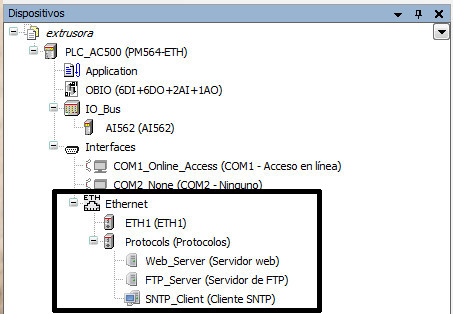
\includegraphics[width=0.5\textwidth]{images/PLC/servicios_plc.jpg}
    \caption[Distintos servicios que dispone el PLC]{Distintos servicios que dispone el PLC. Se pueden instalar distintos servicios de red al PLC: Http, FTP y NTP:}
    \label{fig:plc_servicios}
\end{figure}

En el ordenador, con ayuda de un software cliente FTP se accede aa la IP del PLC que se encuentra en la misma red y se descarga el fichero csv para su posterior estudio (ver Figura \ref{fig:plc_cliente_ftp}).

\begin{figure}[H]
    \centering
    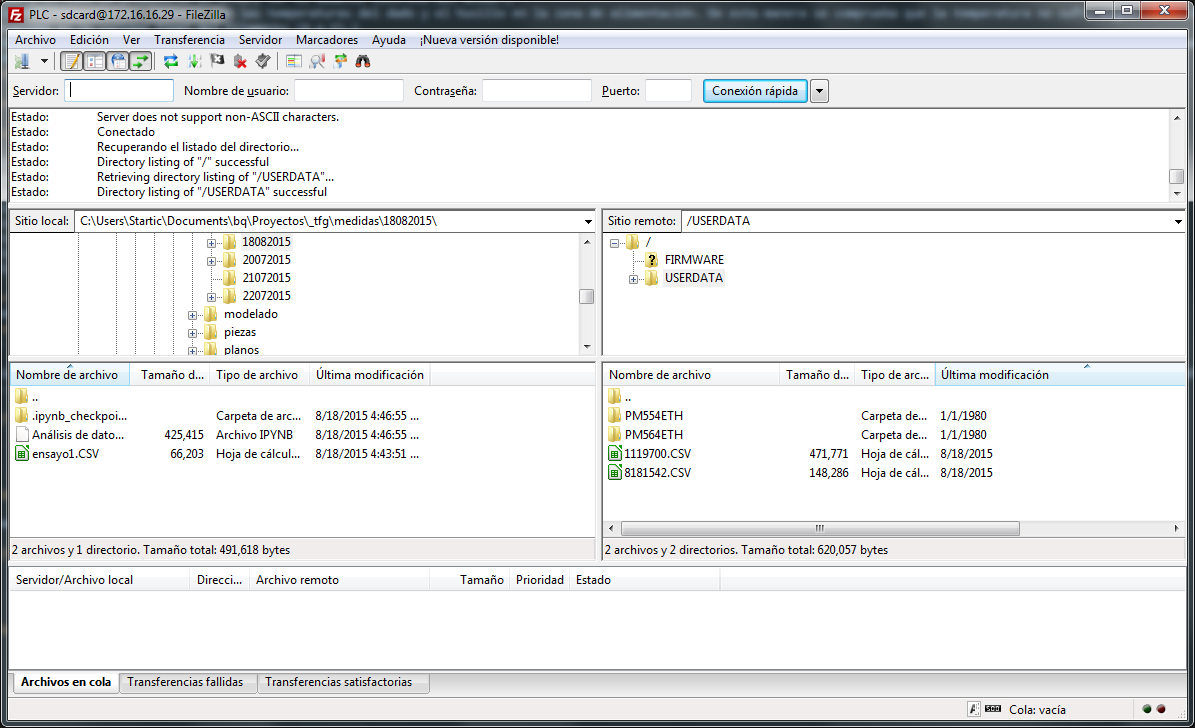
\includegraphics[width=0.95\textwidth]{images/PLC/cliente_ftp.png}
    \caption[Cliente FTP.]{Cliente FTP. Con ayuda de este software, nos podremos conectar a servidores FTP para acceder a los ficheros que hay en el mismo.}
    \label{fig:plc_cliente_ftp}
\end{figure}

\subsection{Visualización web de la producción}
\label{sec:plc_scada}

Para poder visualizar el estado de la producción, se usa una herramienta que incorpora de serie el programa de Abb al igual que el servidor FTP que se vió anteriormente. Esta herramienta, provee un servidor de páginas WEB (ver Figura \ref{fig:plc_servicios}) en la que se puede acceder al estado de variables del programa y se pueden añadir gráficos (ver Figura \ref{fig:plc_visu_web}) que simulen físicamente la planta. Desde esta visualización web se puede:

\begin{itemize}
    \item {Ver temperaturas de Husillo y Dado.}
    \item {Iniciar y parar producción.}
    \item {Controlar marcha del motor del husillo.}
    \item {Ver ruta del fichero en el que se almacenará la información.}
\end{itemize}

\begin{figure}[H]
    \centering
    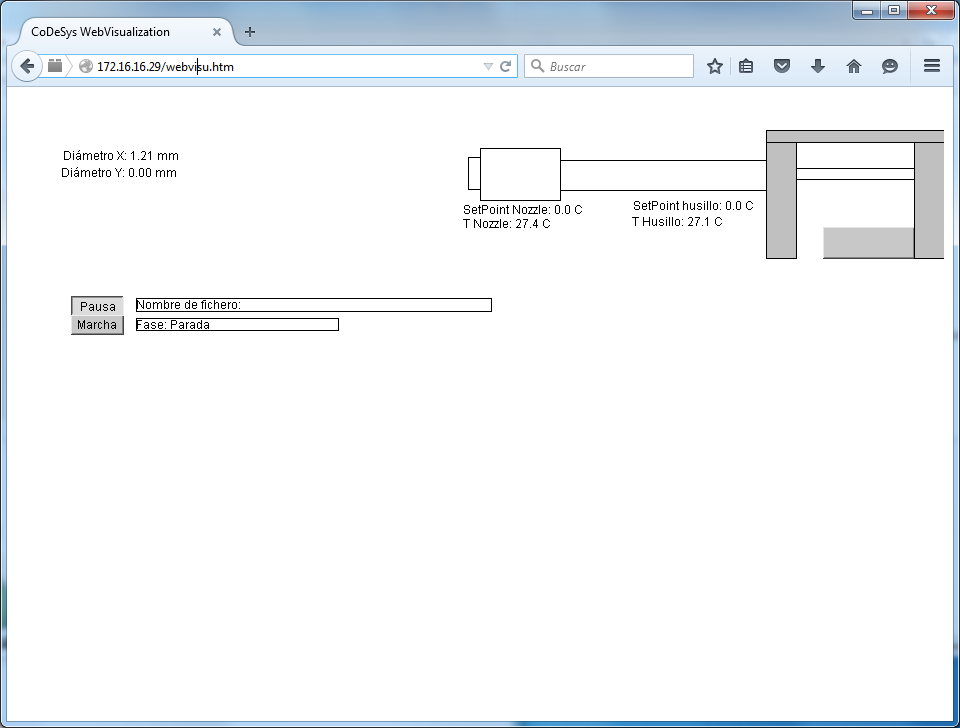
\includegraphics[width=0.95\textwidth]{images/PLC/visu_online.png}
    \caption[Visualización online del sistema.]{Visualización online del sistema.Desde una página web, tenemos acceso a las variables que controlan el proceso.}
    \label{fig:plc_visu_web}
\end{figure}

	%4
	\chapter{Resultados}
\label{cap:resultados}

Como se ha mostrado hasta ahora, se tiene un sistema capaz de registrar la información de una serie de sensores y crear un fichero con esa información. Cuando se incia el planteamiento de este proyecto, el paso final del mismo es implementar el sistema en una linea de extrusión industrial sin embargo, por problemas burocráticos, a la hora de implementar el funcionamiento del mismo, no se tiene acceso a ninguna. \\

Para poder demostrar que el sistema es útil, se decide hacer una maqueta de una extrusora para poder comprobar cómo con el sistema diseñado podemos realizar un estudio avanzado de los problemas que tenemos a la hora de fabricar filamento.\\


\section{Filastruder-sensor diámetro-bobinadora}
\label{sec:FSB}

Como primera aproximación e intentando asemejar el esquema de producción que tienen en la fábrica de Huesca se va a seguir el esquema mostrado en la figura \ref{fig:esquemap_FSB}:

\begin{figure}[H]
    \centering
    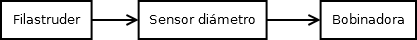
\includegraphics[width=0.6\textwidth]{images/producciones/Diagram1.png}
    \caption[Esquema de producción Filastruder-sensor de diámetro-bobinadora.]{Esquema de producción Filastruder-sensor de diámetro-bobinador.}
    \label{fig:esquemap_FSB}
\end{figure}

La boquilla de la filastruder es de 3mm, de esta manera se tiene margen suficiente para regular el filamento aplicando una fuerza de tracción según sale de la extrusora y se va enfriando. A la hora de trabajar con una técnica de conformado como es esta, es muy importante que la velocidad de salida sea lo más constante posible y también hay que tener en cuenta que se producen cambios en el material tanto de tamaño como de forma según sale de la extrusora. Tres de estos cambios que afectan al material son: \cite{tecno_polimeros}

\begin{itemize}
	\item {\textbf{Tensionado}: Habitualmente, el material es recogido por sistemas de almacenamiento consistentes en rodillos que aplican una tensión. Esto hace que el tamaño del material varié en función de esa tensión. Nos ayudaremos de esta característica para intentar regular el diámetro final del filamento. El tamaño del diámetro tendrá una relación inversamente proporcional a la velocidad.}
	\item {\textbf{Relajación}: Dentro de la extrusora, el material soprta esfuerzos normales y  al salir por la boqquilla se relaja. Esta relajación será mayor, en función del gradiente de temperatura que haya entre la boquila y el ambiente.
		\begin{figure}[H]
	        \centering
	        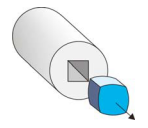
\includegraphics[width=0.2\textwidth]{images/producciones/relajacion.png}
	        \caption[Cambio de tamaño debido a la relajación del material.]{Cambio de tamaño debido a la relajación del material. Fuente \cite{tecno_polimeros}}
	        \label{fig:prod_relajacion}
		\end{figure}
	}
	\item {\textbf{Enfriamiento}: A medida que el material se va enfriando, se va generando una contracción en el perfil del mismo. Está contraccion depende de la velocidad de enfriamiento del material. Por ello, no habrá la misma contracción en una zona gruesa donde haya más material, que en una fina.
		\begin{figure}[H]
	        \centering
	        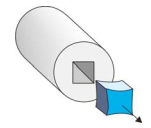
\includegraphics[width=0.2\textwidth]{images/producciones/contraccion.png}
	        \caption[Cambio de tamaño debido a la contraccion del material.]{Cambio de tamaño debido a la contraccion del material. Fuente \cite{tecno_polimeros}}
	        \label{fig:prod_contraccion}
		\end{figure}
	}
\end{itemize}

\subsection{Resultados}
Vamos a comprobar el funcionamiento del sistema con el control de regulación de la propia filawinder, en la que intenta mantener el filamento en una determinada altura y en función de esa altura, aplicar más o menos velocidad de bobinado. Para esta primera producción se usarán todos los pellets reciclados como materia prima, no se mezclará con PLA transparente, para así ver si el funcionamiento de la filastruder es el correcto.\\

Una vez llegado a la consigna de temperatura de 150ºC se comienza a extruir PLA reciclado y se almacena en la bobina. A simple vista, se ve que la velocidad mínima de bobinado hace que el filamento salga demasiado delgado y se generan demasiadas tensiones en el bobinado del mismo. No obstante, analizaremos los resultados obtenidos. Para el análisis del fihero CSV generado, se usará la herramienta IPython con las librerias, Numpy y Scypi, con los que de manera rápida obtendremos unas conclusiones.\\

Las condiciones iniciales del ensayo son:

	\begin{itemize}
		\item Hora de inicio: 11:50
		\item Hora de fin: 12:20
		\item Temperatura de extrusión: 150ºC
	\end{itemize}

Las medidas obtenidas en el ensayo son:

\begin{table}[H]
	\centering
	\begin{tabular}{ccc}
		{\bf } & {\bf Diámetro X} & {\bf Diámetro Y} \\ \hline
		Medidas & 1110.000000 & 1110.000000 \\
		Media (mm) & 1.17 & 0.91 \\
		Desviación estandar & 0.39 & 0.51 \\
		Mínimo (mm) & 0.01 & 0.00 \\
		Máximo (mm) & 1.92 & 1.74
	\end{tabular}
	\caption{Resultados obtenidos en la producción}
	\label{tab:result1}
\end{table}

Cómo podemos comprobar obtenemos una media aritmética de filamento de $ \bar{x} = 1.17mm $  mm con una desviación estandar $\sigma = 0.39$. Representando las medidas de los ejes X e Y podemos comprobar que el resultado no es el deseado:

\begin{figure}[H]
	\centering
	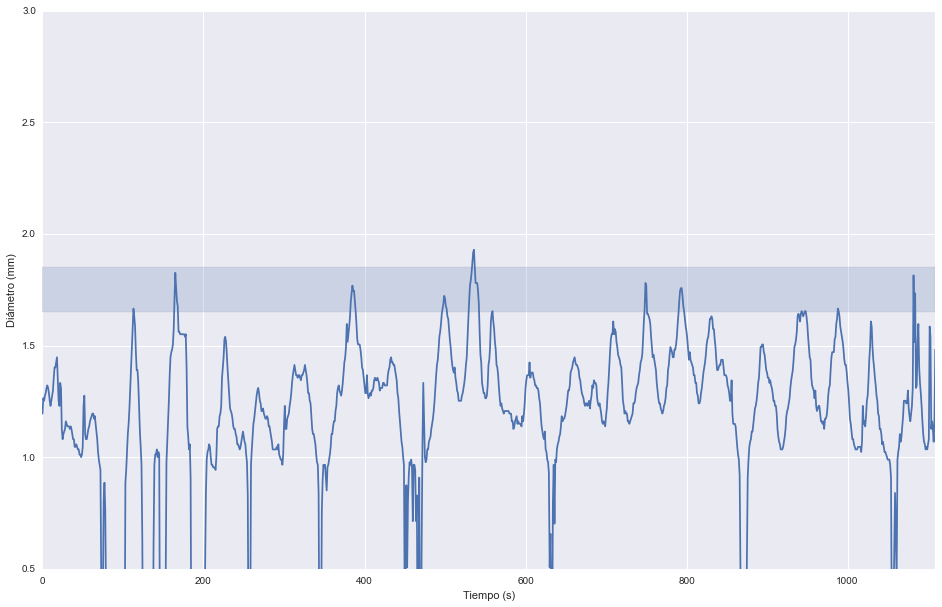
\includegraphics[width=0.8\textwidth]{images/producciones/16062015/output_9_1.png}
	\caption{Representación de las medidas de los ejes X e Y.}
	\label{fig:prod_ejes}
\end{figure}

Sólo un pequeño número de muestras están por dentro de los márgenes de calidad establecidos por BQ (Max = 1.85mm ; Min = 1.65mm). Además, si representamos los datos en un diagráma de cajas, vemos que hay mucha variación entre los dos ejes:
\begin{figure}[H]
    \centering
    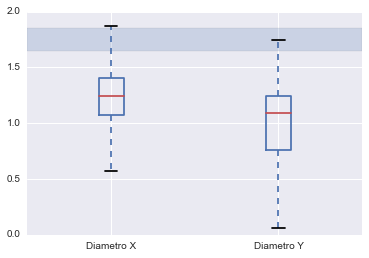
\includegraphics[width=0.5\textwidth]{images/producciones/16062015/output_10_1.png}
    \caption{Diagrama de cajas de las medidas de los ejes X e Y.}
    \label{fig:prod_boxplot}
\end{figure}

Después de los resultados obtenidos en el experimento, descartamos que con este esquema de producción y los materiales disponibles, lleguemos a regular el diámetro de salida de una forma óptima, por tanto se trata de obtener otro esquema de producción para ganarantizar mejores resultados.

\section{Filastruder-sensor diámetro-Tractora}
\label{sec:FST}

En una de las pruebas de extrusión de filamento, se va estirando a mano según va saliendo de la filastruder y se comprueba que, traccionando del hilo a una distancia cercana de la boquilla y una vez enfriado, se puede llegar a regular el diámetro final. Por ello, se trata de investigar en esta linea, diseñar un sistema capaz de traccionar el filamento a medida que va saliendo de la boquilla.

\begin{figure}[H]
    \centering
    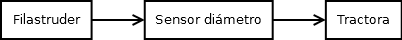
\includegraphics[width=0.6\textwidth]{images/producciones/Diagram2.png}
    \caption{Esquema de producción filastruder-sensor de diámetro-tractora.}
    \label{fig:esquemap_FST}
\end{figure}

Con el conocimiento adquirido al diseñar la peletizadora (ver anexo \ref{ane:peletizadora}) se diseña una unidad tractora que irá colocada después de la filastruder, la cual, deberá ir traccionando del filamento independientemente del diámetro del mismo. Así mismo, deberemos ser capaces de regular la velocidad de una forma más precisa que como lo hicimos con la peletizadora. En el anexo \ref{ane:tractora} se detalla el proceso seguido a la hora del diseño de la tractora.\\

Por tanto, podemos pasar a instalar la tractora en la maqueta.

\begin{figure}[H]
    \centering
    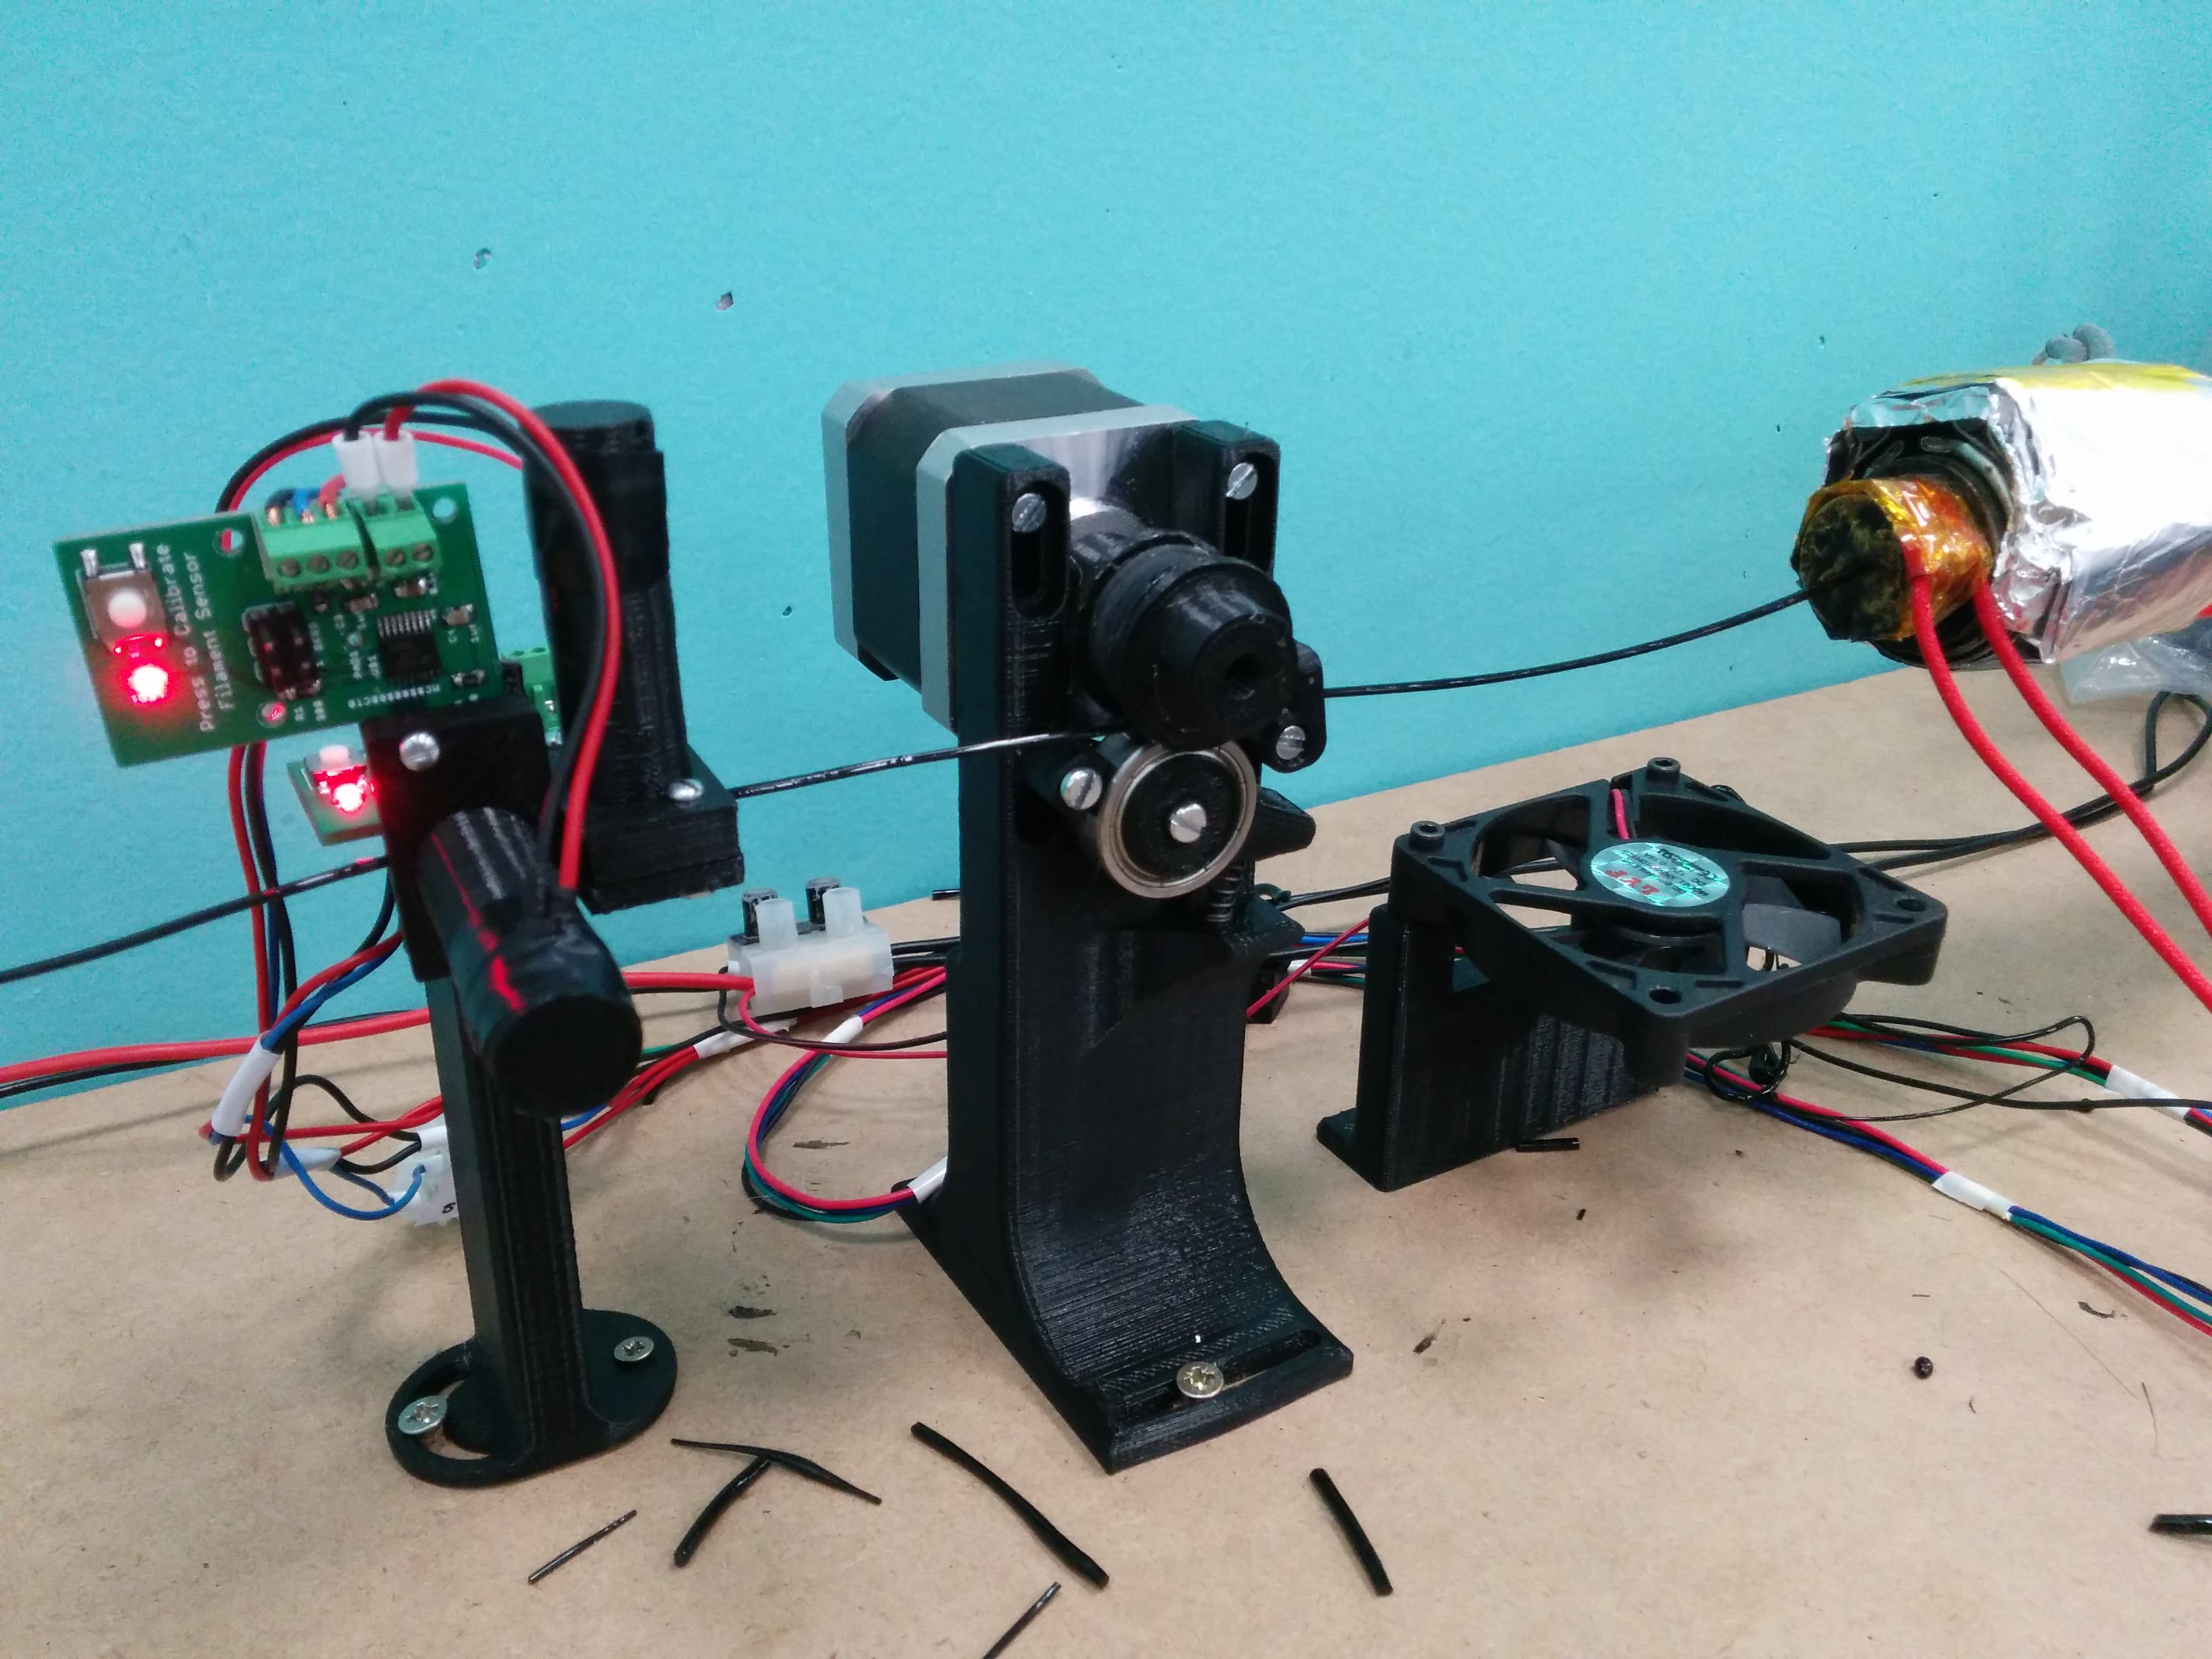
\includegraphics[width=0.6\textwidth]{images/producciones/tractora/IMG_20150709_130326.jpg}
    \caption{Montaje final filastruder-tractora-sensor}
    \label{fig:montaje_final}
\end{figure}

\subsection{Resultados}

Usando pellets reciclados, se pasa a hacer una producción de filamento, para comprobar que el diseño de la tractora es el correcto. El ensayo que se va a realizar consiste en:

\begin{itemize}
    \item{Establecer una temperatura de 135ºC en el extrusor.}
    \item{Llenar la tolva que incluye de serie la extrusora con 42gr de pellets reciclados.}
    \item{Extruir filamento registrando los datos para su posterior análisis.}
    \item{Cambiar la velocidad de tracción para comprobar la relación final en el diámetro. Se establecera una velocidad de 1RPM y 3RPM}
\end{itemize}

Se está alrededor de seis minutos extruyendo filamento, sin embargo, debido a un exceso en el diámetro del filamento, hace que este no entre por el sensor de diámetro y sea necesario parar, sin embargo podemos estudiar los datos obtenidos.
Tras el ensayo, los resultados obtenidos son los siguientes:

\begin{table}[H]
    \centering
    \begin{tabular}{cc}
               & Diámetro X \\ \hline
    Medidas    & 203        \\
    Media (mm) & 1.59       \\
    Desviación estandar & 0.25\\
    Mínimo (mm)   & 1.08       \\
    Máximo (mm)   & 2.19      
    \end{tabular}
    \caption{Datos obtenidos en el ensayo del día 20 de Julio}
    \label{tab:20007105-dat}
\end{table}

\begin{figure}[H]
    \centering
    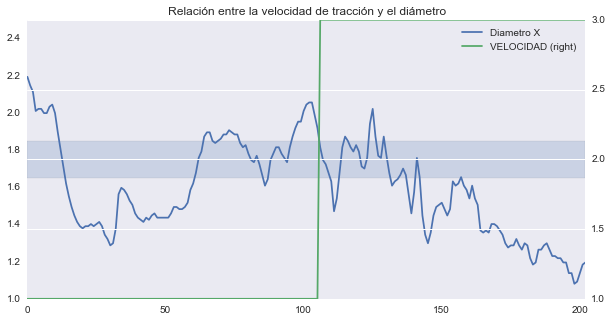
\includegraphics[width=0.99\textwidth]{images/producciones/20072015/graficas.png}
    \caption{Gráfica con los datos de la producción}
    \label{fig:2007105-graf}
\end{figure}

En la gráfica anterior vemos los datos obtenidos del diámetro del eje X. Se ve claramente, que hay una variación muy pronunciada al tener una velocidad de tracción constante, esto es un problema en el diseño de la filastruder ya que, a una velocidad de tracción constante, el diámetro debería serlo también. Durante el ensayo, se ha notado física y acústicamente que la extrusión no es constante, por ello, pensamos que el funcionamiento de la filastruder, que a simple vista parecía correcto, no puede llegar a proporcionarnos los resultados que necesitamos. Se instala un encoder mediante un imán, un sensor de efecto hall y un arduino a la filastruder, para cercionarnos de que la velocidad es constante.

\begin{figure}[H]
    \centering
    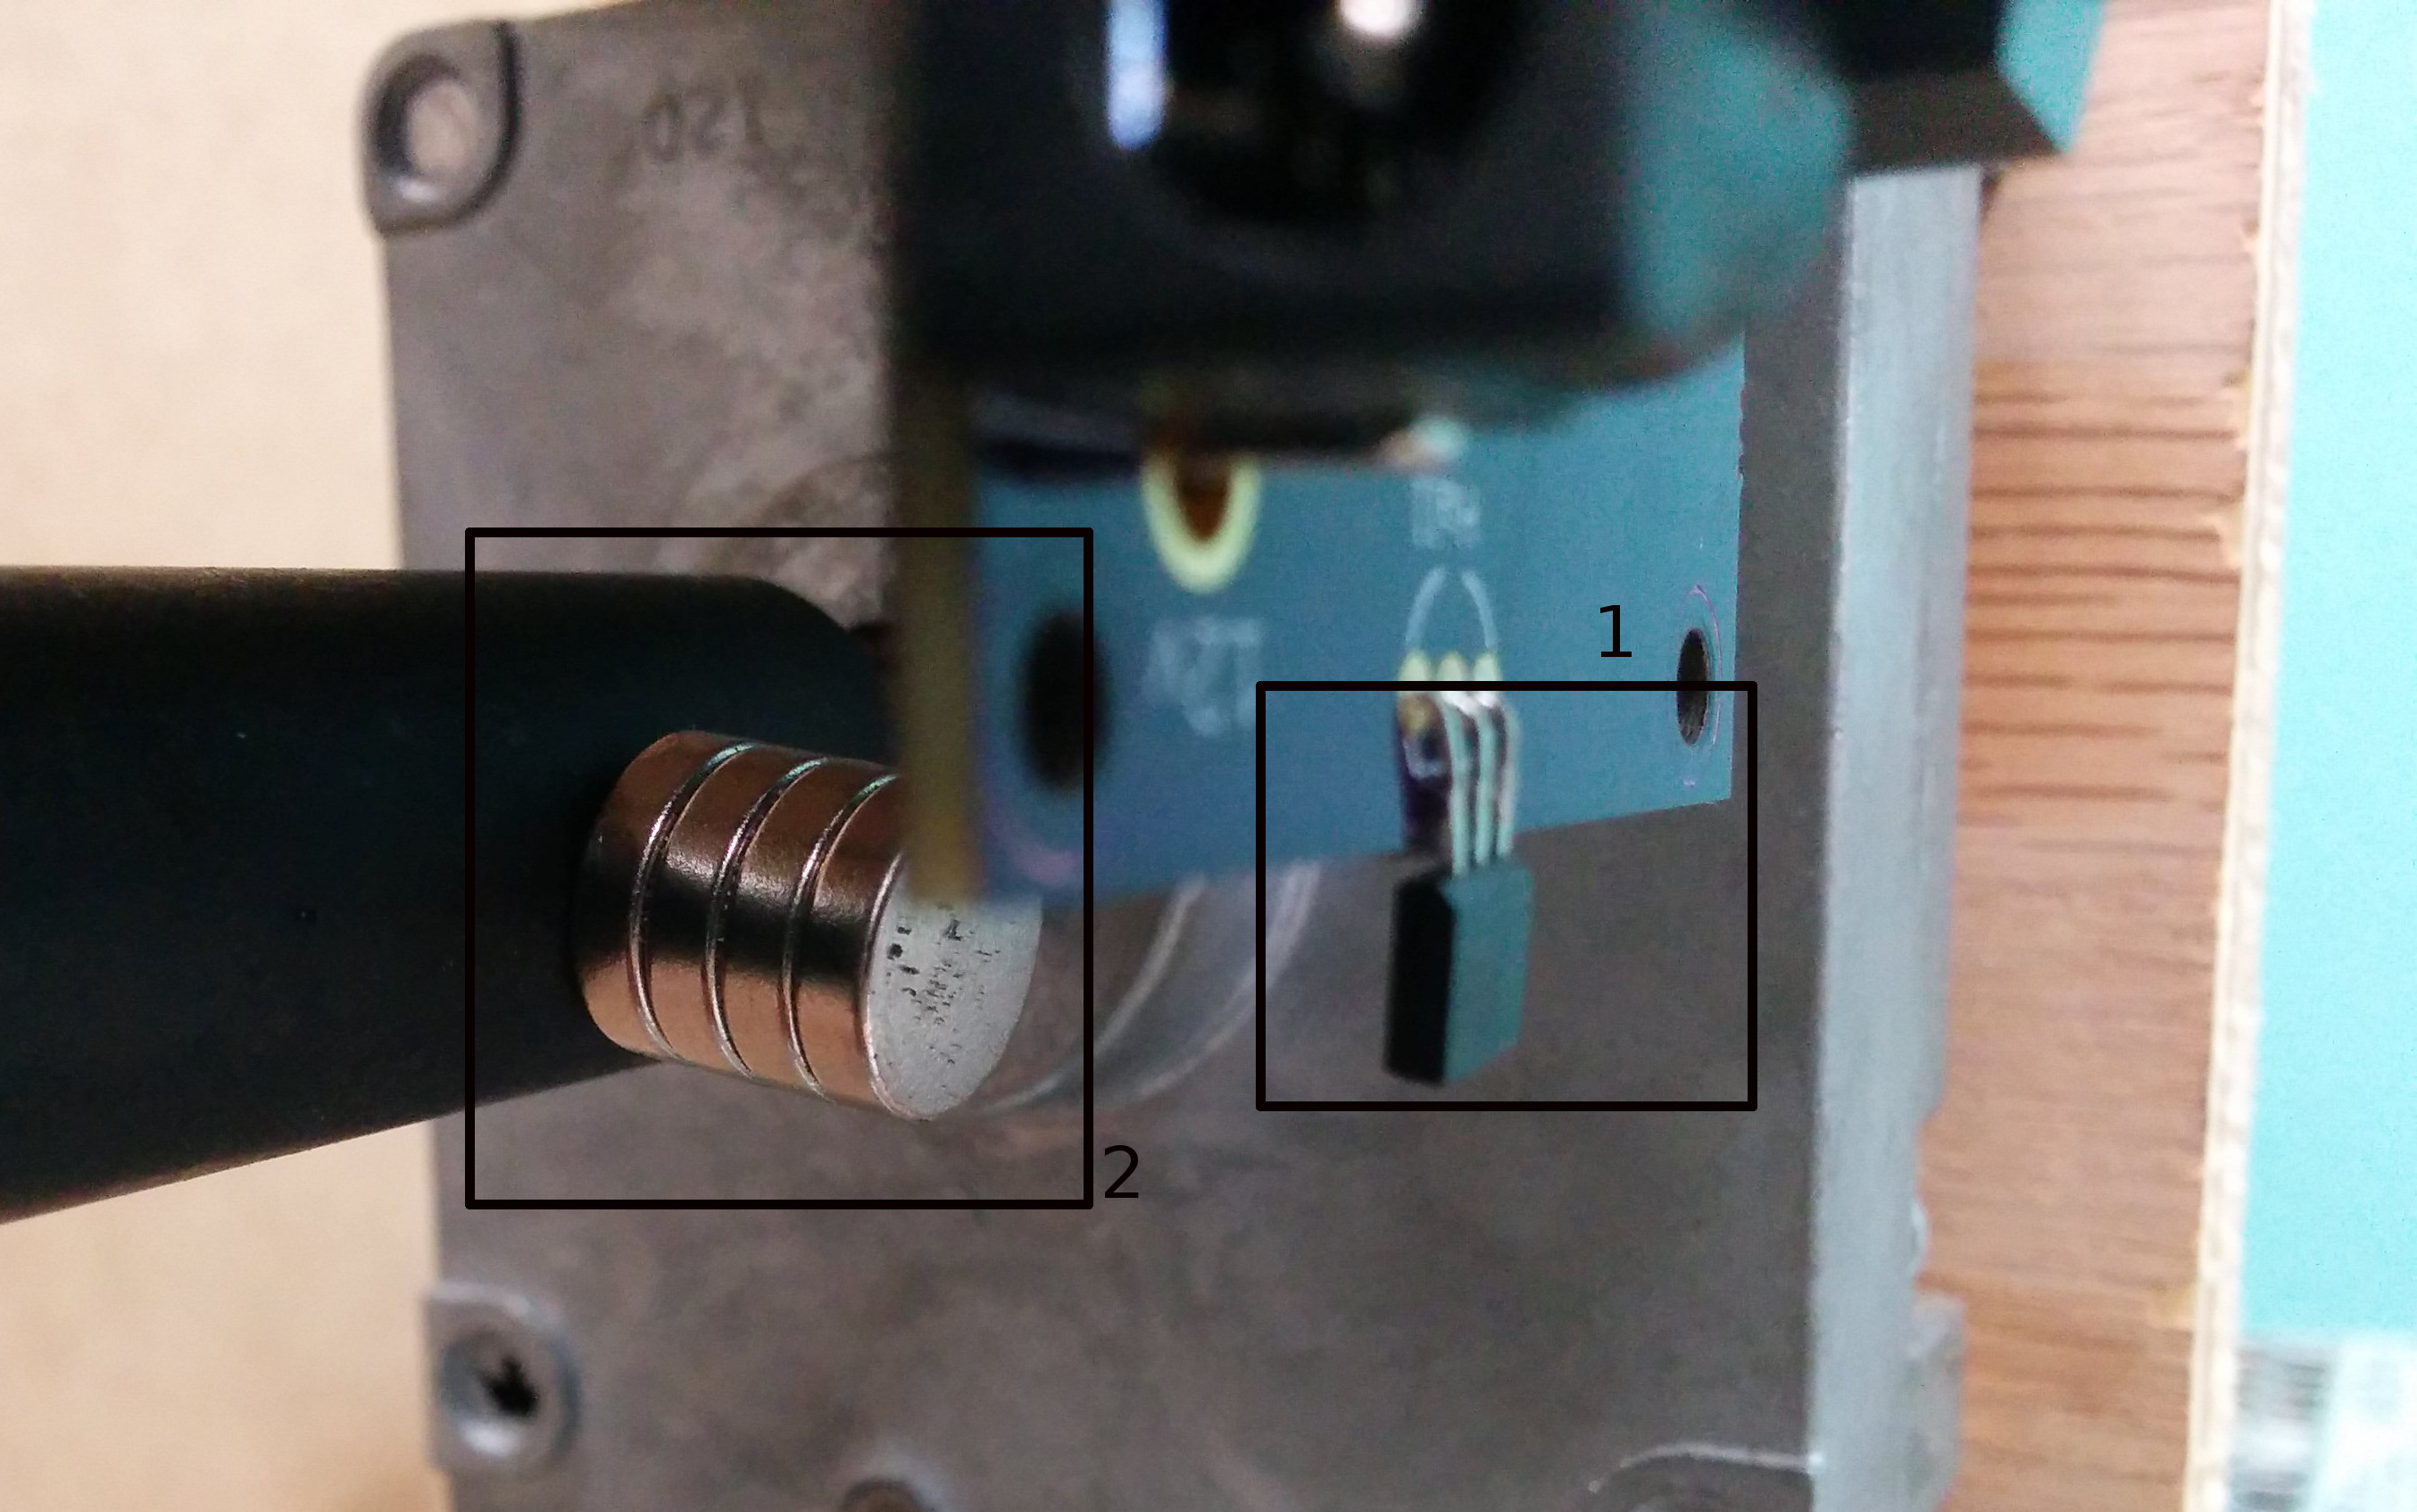
\includegraphics[width=0.8\textwidth]{images/producciones/20072015/IMG_20150721_110502.jpg}
    \caption{Encoder instalado en la filastruder.}
    \label{fig:2007105-enc}
\end{figure}

Se extruye una cantidad de filamento sin medir el diámetro, tan sólo registrando la velocidad con la que gira el husillo y los datos proporcionados son los siguientes:

\begin{figure}[H]
    \centering
    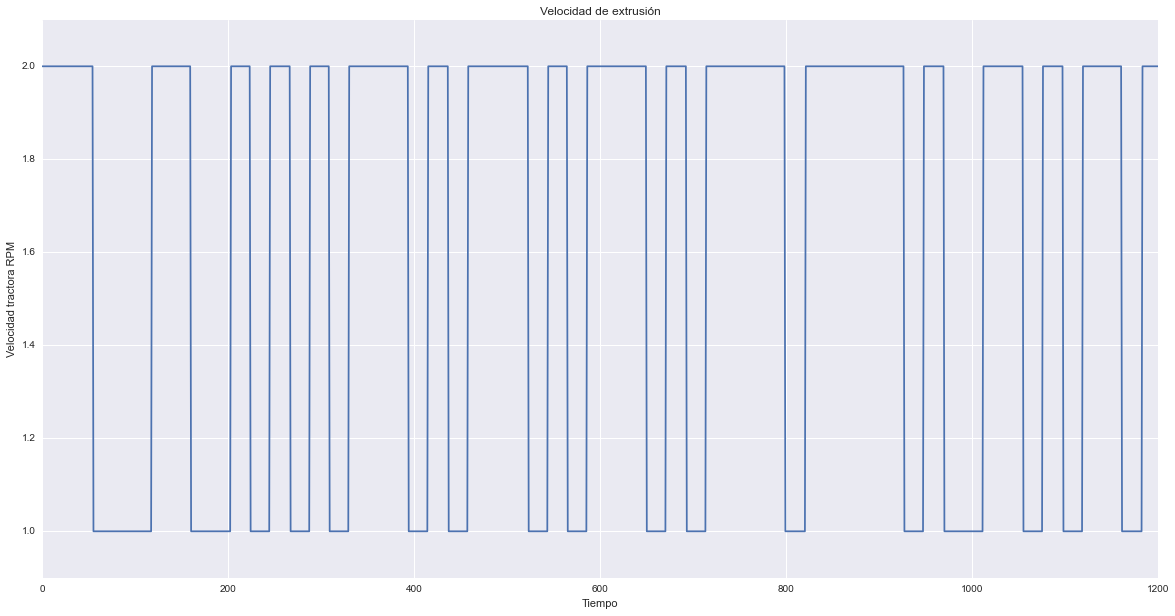
\includegraphics[width=0.99\textwidth]{images/producciones/20072015/RPM_tract.png}
    \caption{Velocidad de la extrusora.}
    \label{fig:2007105-grafenc}
\end{figure}

Se ve claramente, que la velocidad de giro no es constante, variando entre 1 y 2 RPM. El motor que hace girar el husillo está conectado directamente a 12V y no se tienen ningún control sobre él. Además mecánicamente, el motor está conectado al husillo mediante una caja reductora, la cual no podemos cambiar. Para no alargar la duración del proyecto e intentar avanzar en el control se van a tomar las siguientes medidas:

\begin{itemize}
    \item{Usar una mezcla de granza de PLA natural (70\%) con pellets reciclados de filamento (30\%) (ver figura \ref{fig:2007105-mezc}). Se usará granza de PLA natural, el cual tiene una forma más redondeada que los pellets reciclados, haciendo más fácil el avance dentro del cañón. Se usa una mezcla con los pellets reciclados, ya que el sensor de diámetro que usamos, no funciona con filamento transparente, por ello, debemos tintar el filamento}
	    \begin{figure}[H]
		    \centering
		    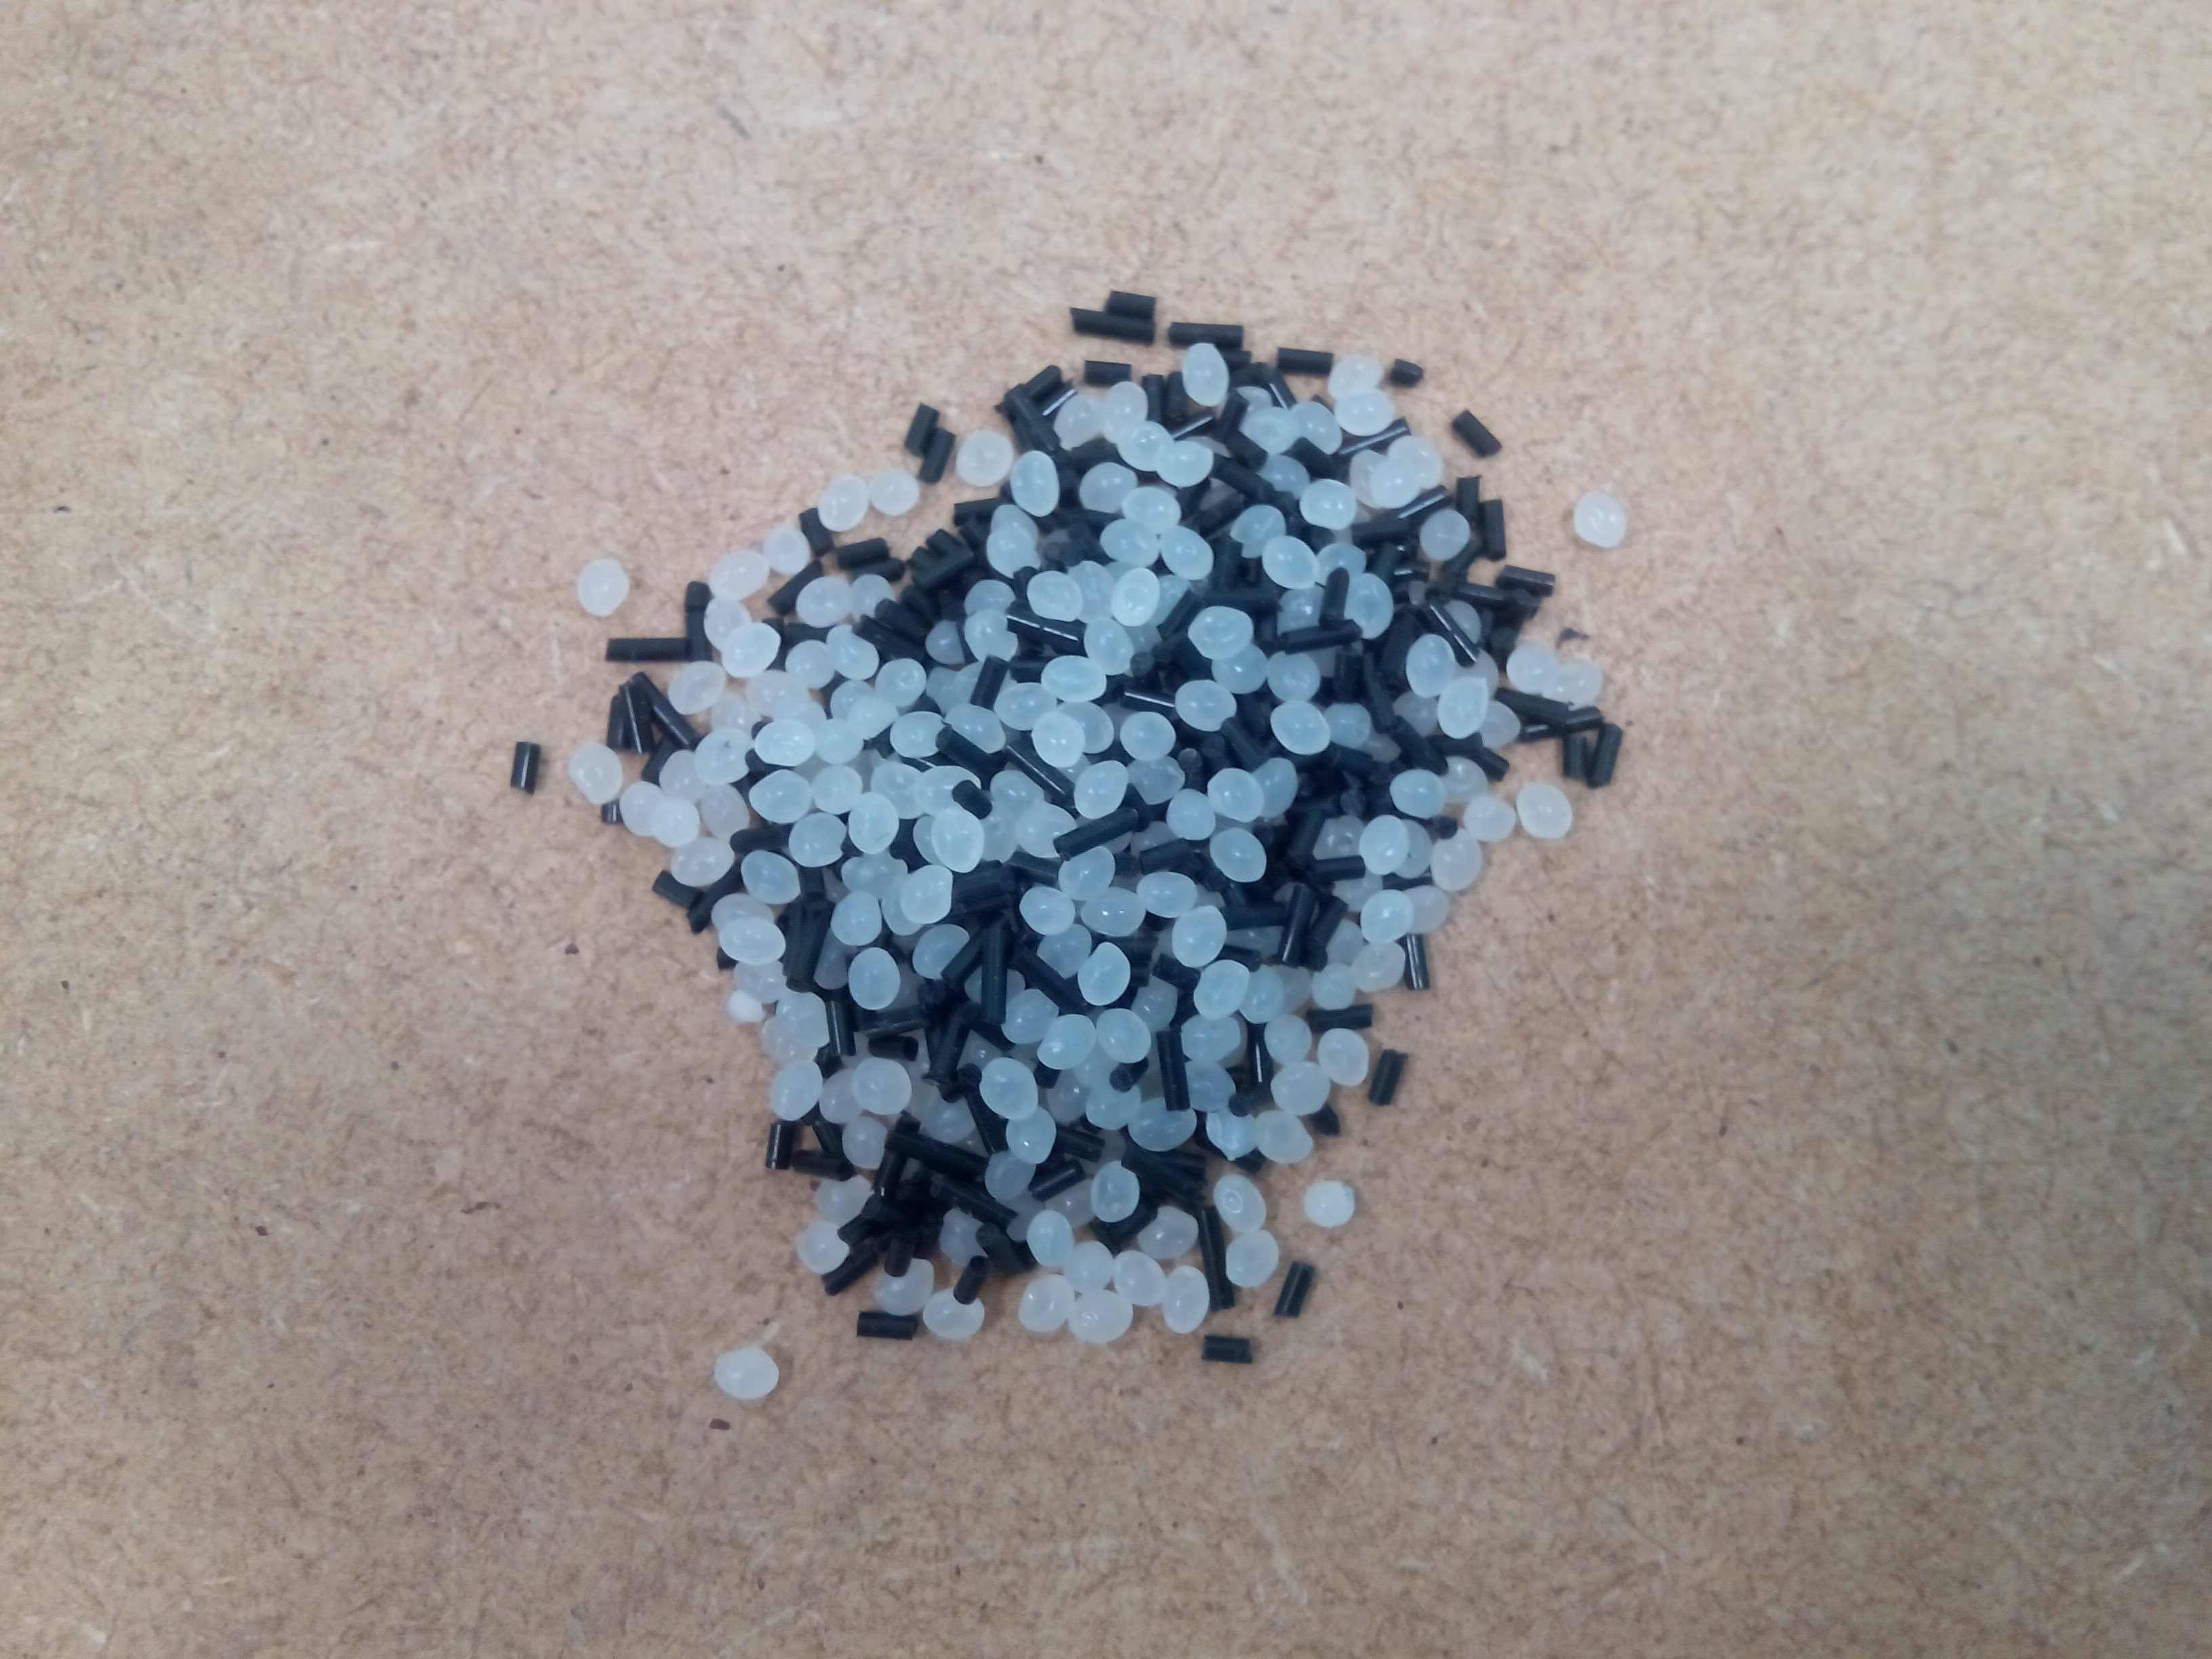
\includegraphics[width=0.6\textwidth]{images/producciones/20072015/IMG_20150903_155859.jpg}
		    \caption{Mezcla de granza con pellets reciclados.}
		    \label{fig:2007105-mezc}
		\end{figure}
    \item{Antes de hacer una producción de filamento, la granza de PLA que se vaya a usar, se va a secar en un horno a una temperatura de 80ºC durante, al menos, tres horas antes de la producción. Esto es debido a que si el PLA tiene un alto porcentaje de humedad, hará que la extrusión del material no sea el adecuado, afectando directamente en el acabado final.}
    \item{Se va a diseñar una tolva de alimentación mayor, para que la capacidad de granza aumente, y se ejerza mayor presión a la entrada del extrusor, para que de ese modo, la alimentación de la granza se lo más constante posible. El tamaño de almacenamiento máximo ha pasado de 42gr a 150gr (ver figura \ref{fig:tolv_montaj}).}
\end{itemize}

\begin{figure}[H]
    \centering
    \begin{subfigure}[b]{0.45\textwidth}
        \centering
        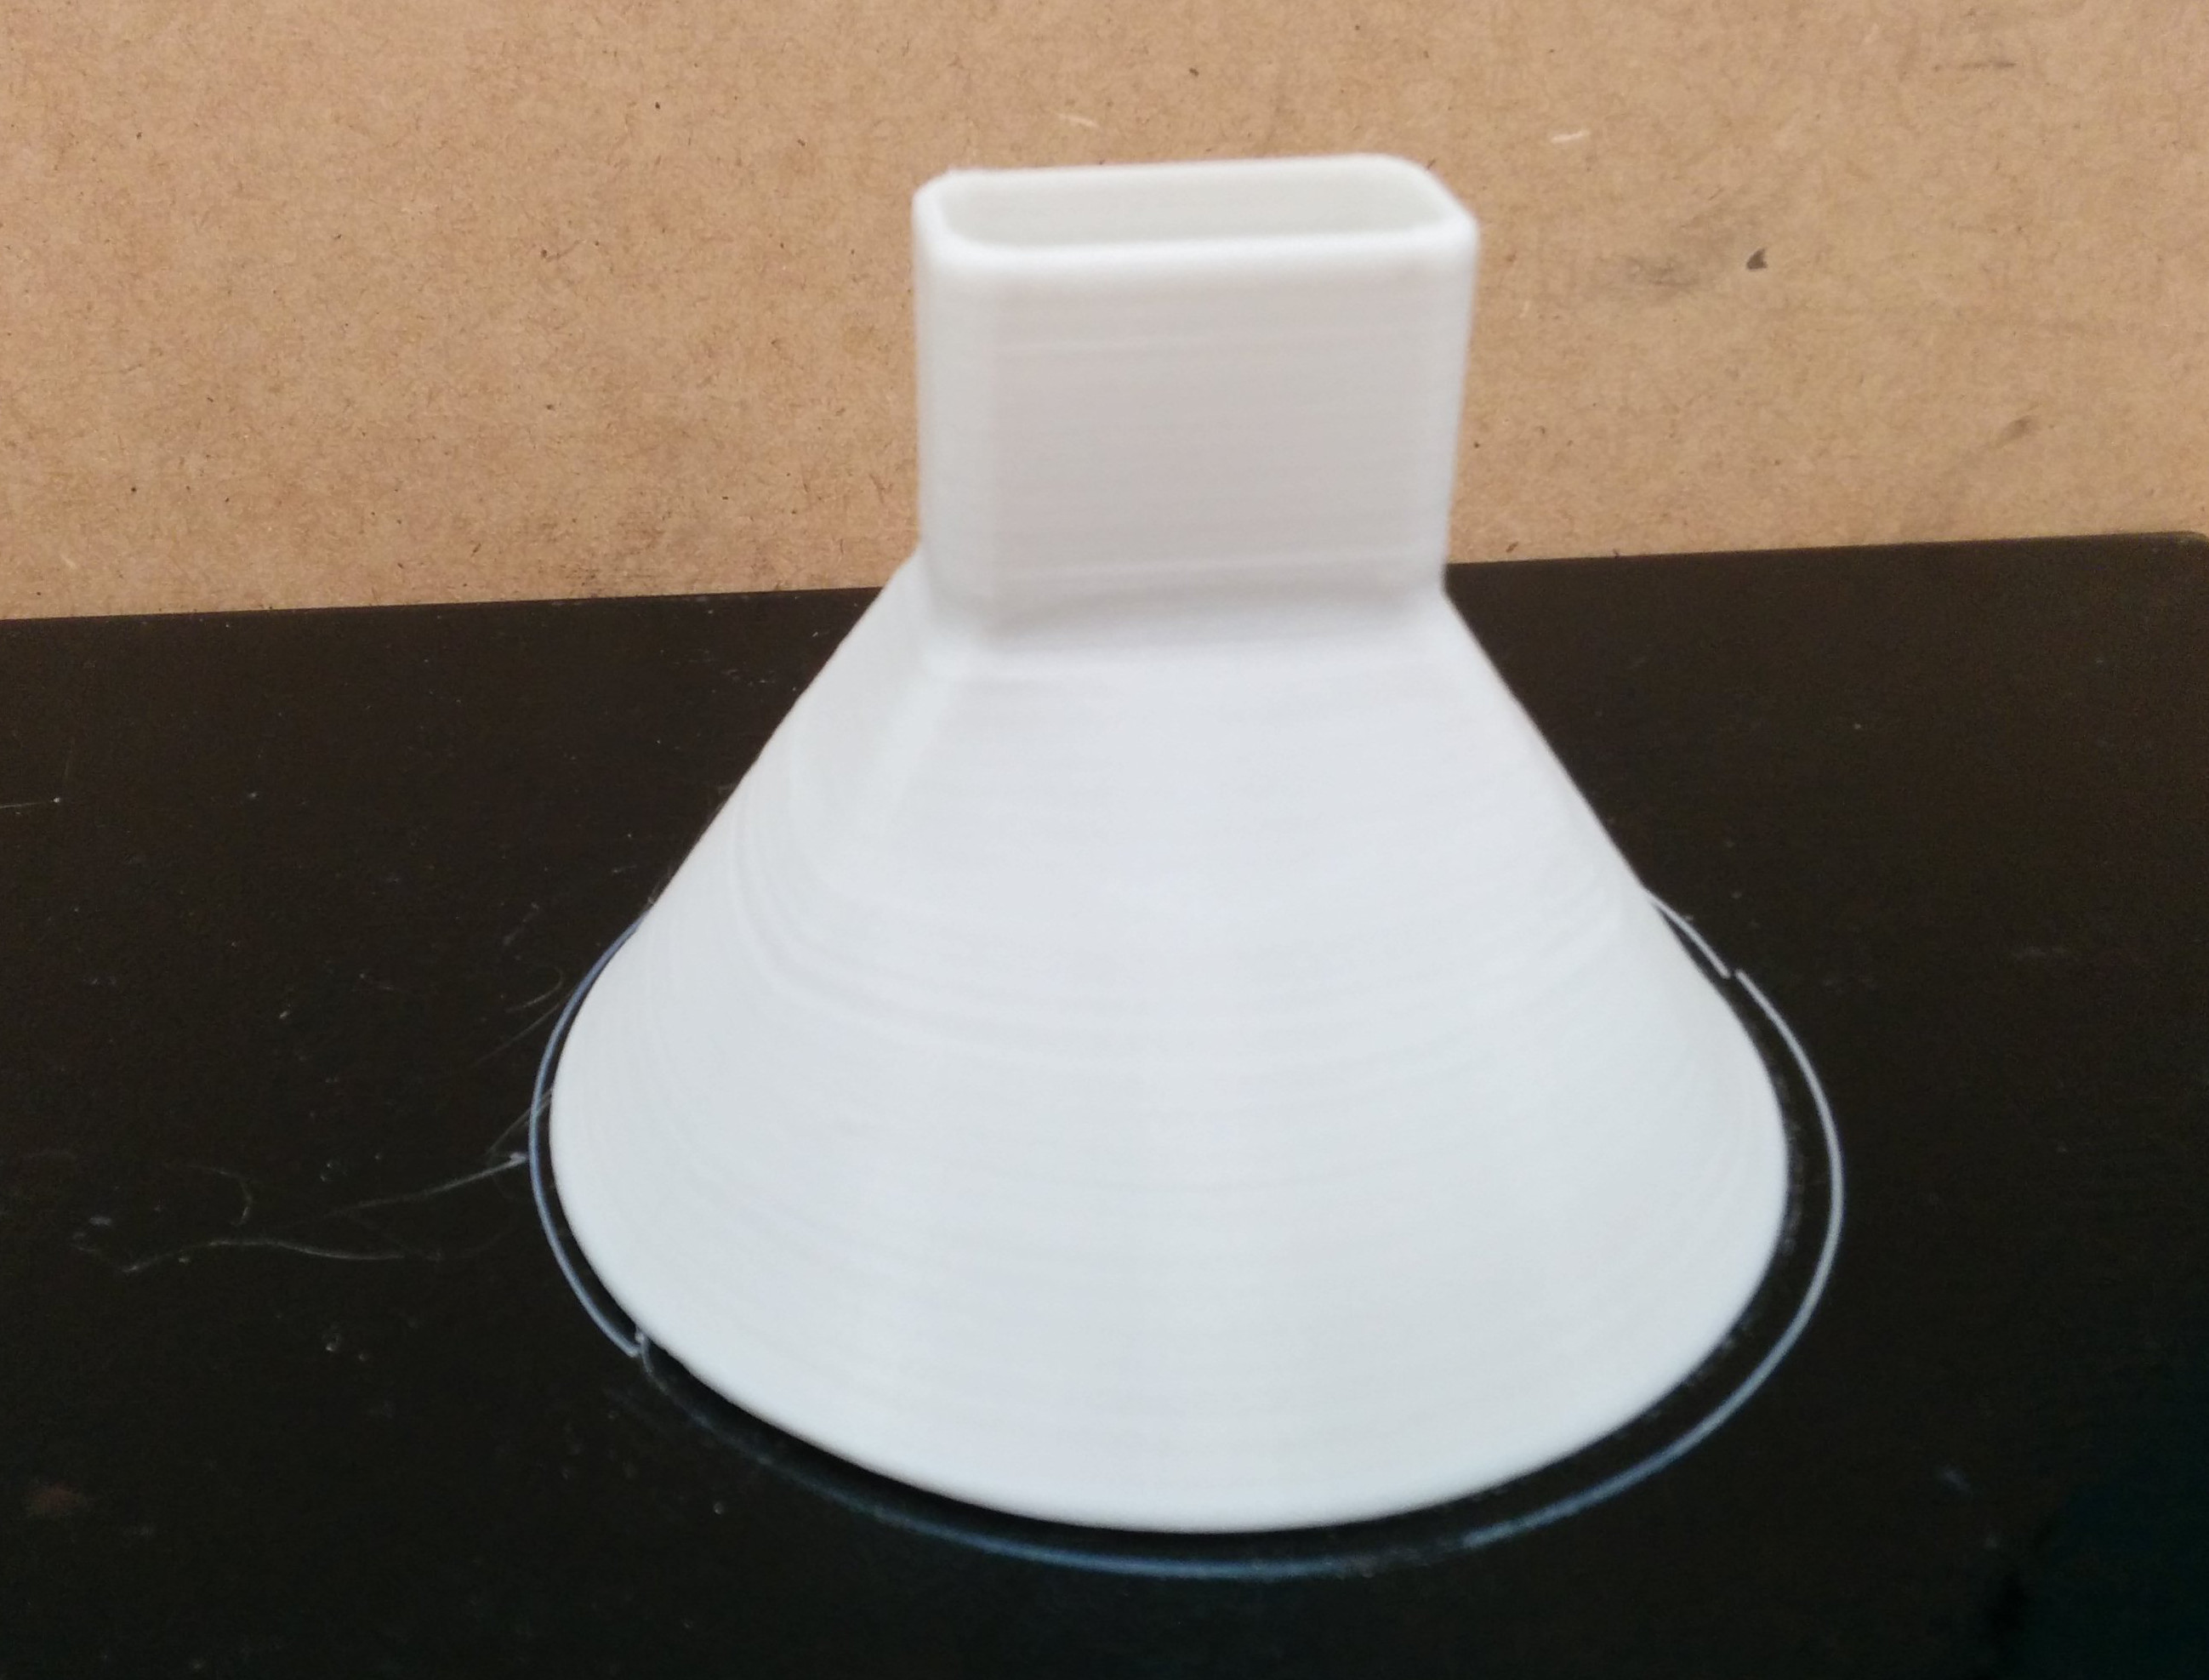
\includegraphics[width=\linewidth]{images/producciones/20072015/IMG_20150721_121831.jpg}
        \label{fig:tolva-impresa}
    \end{subfigure}
    ~
    \begin{subfigure}[b]{0.45\textwidth}
            \centering
        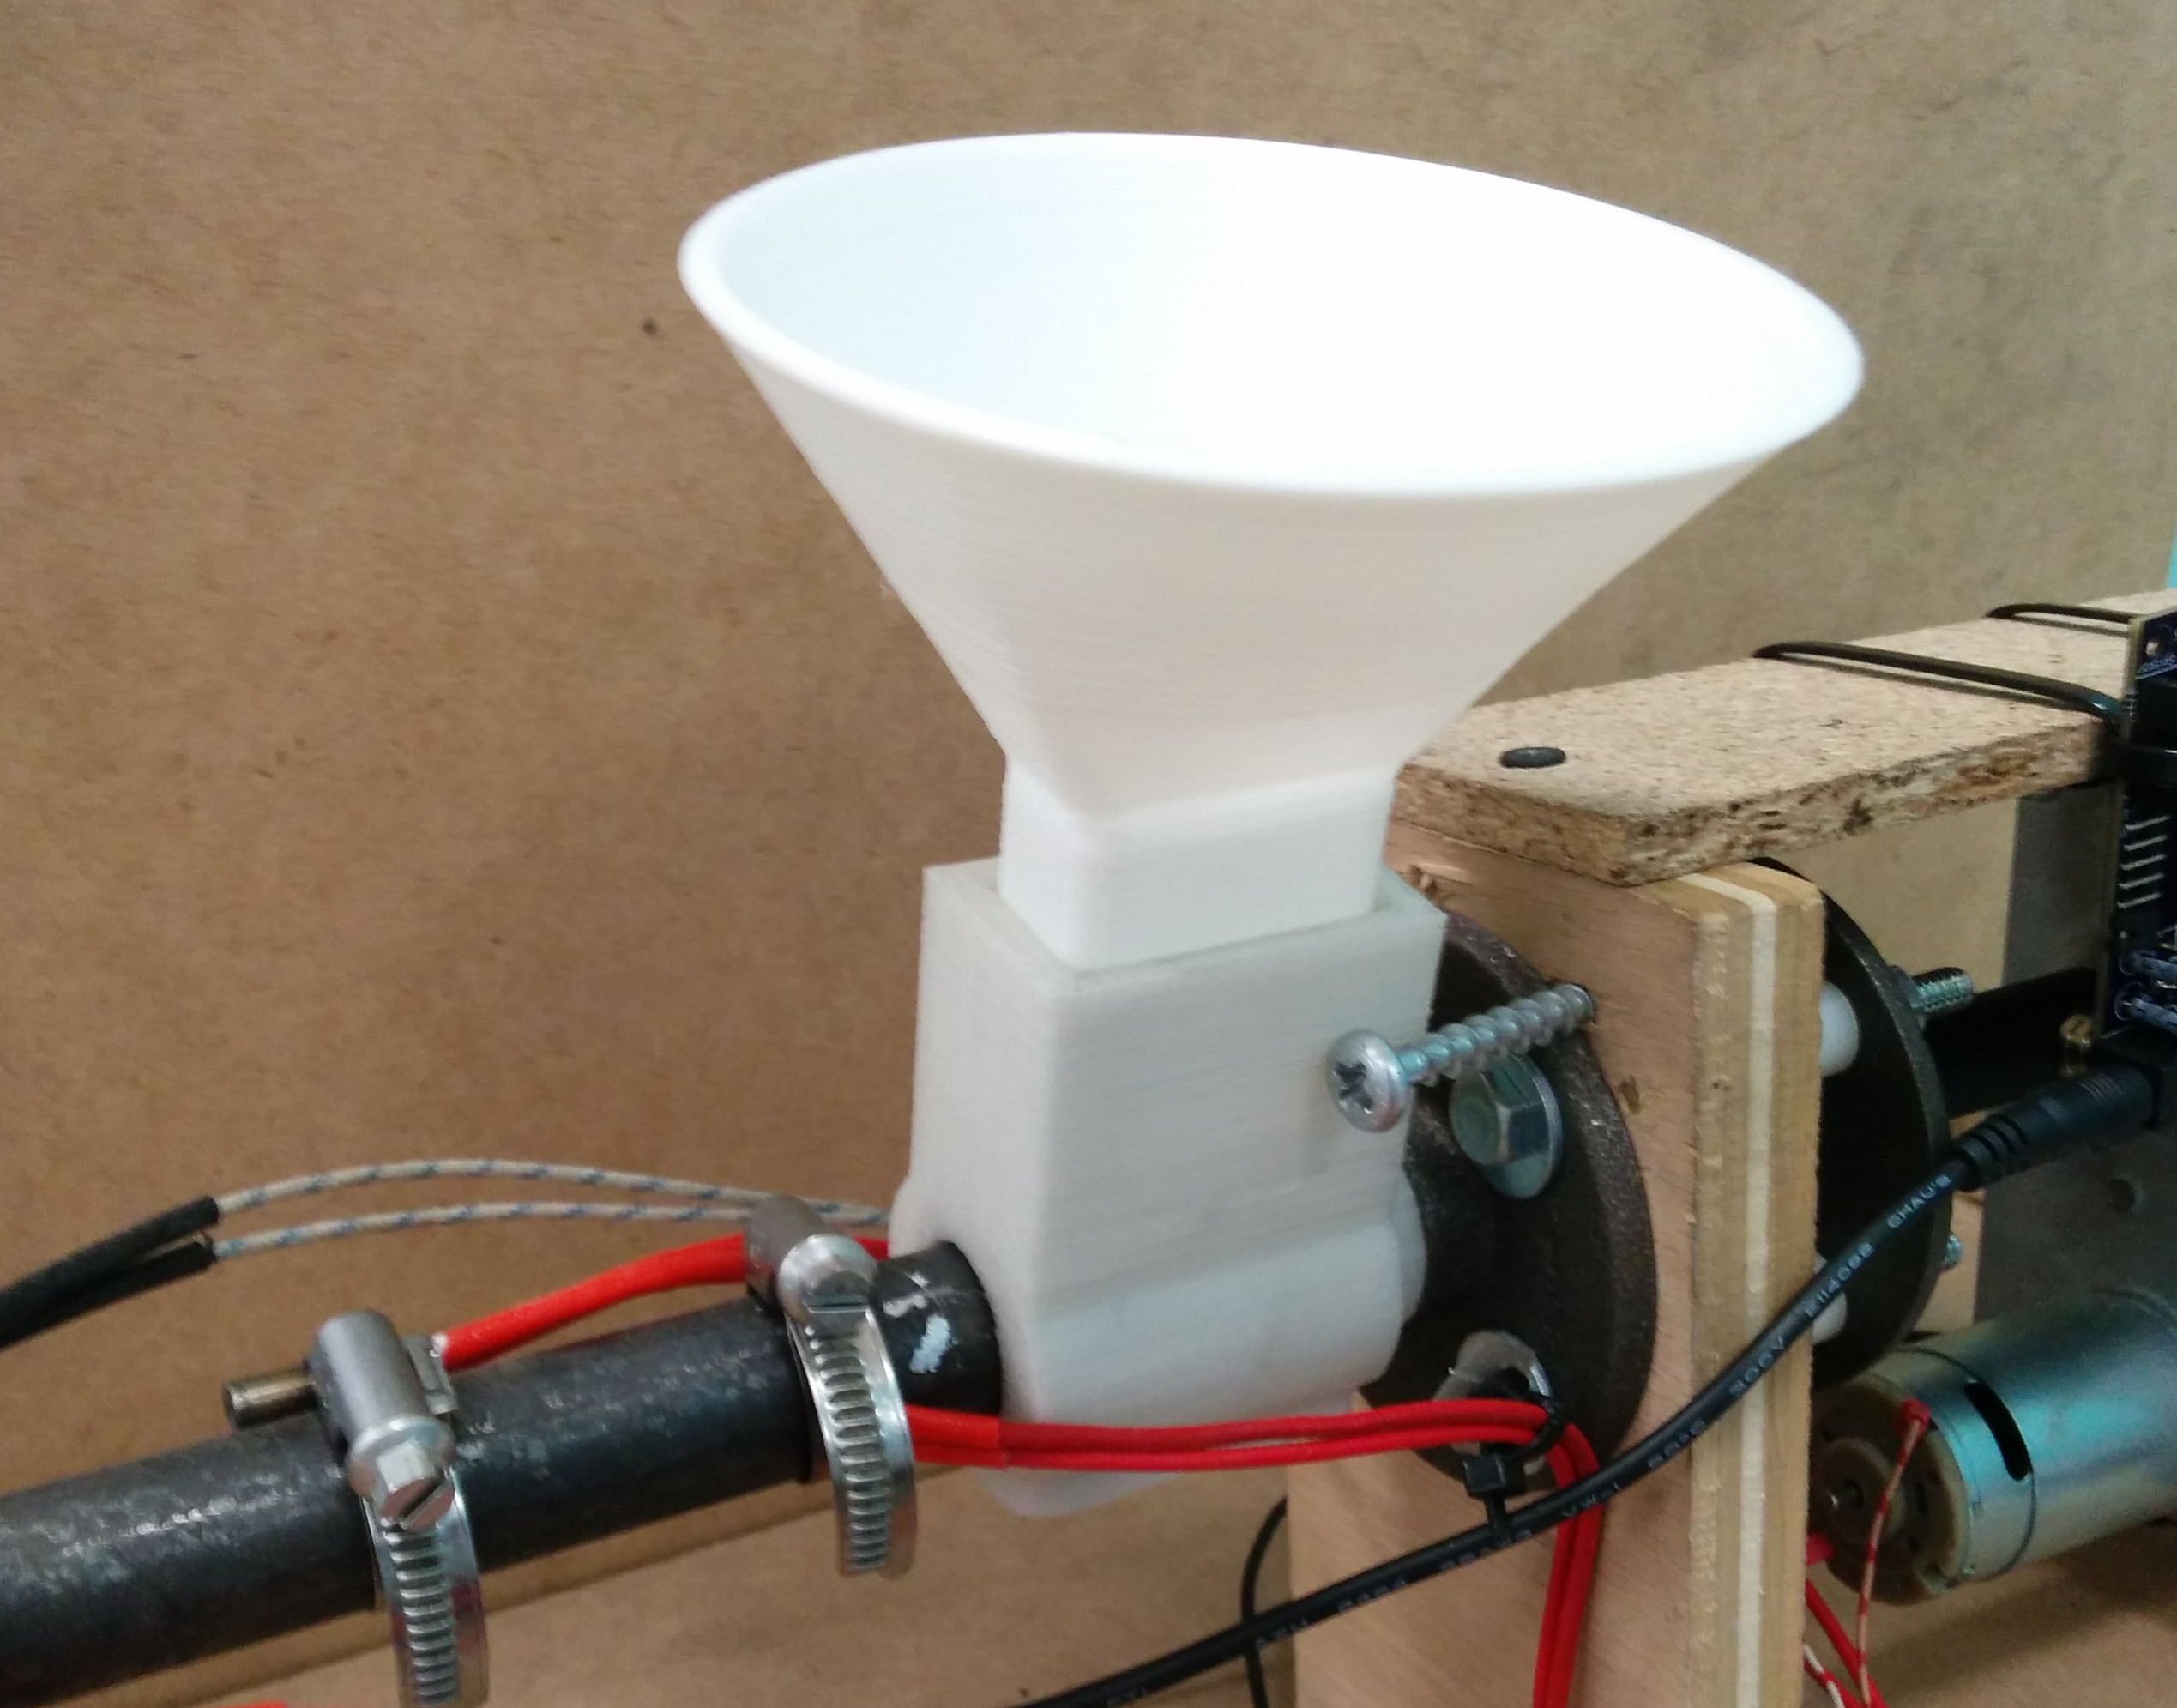
\includegraphics[width=\linewidth]{images/producciones/20072015/IMG_20150721_121904.jpg}
        \label{fig:tolva-montada}
    \end{subfigure}
    \caption[Diseño y montaje de una tolva de mayor capacidad.]{Diseño y montaje de una tolva de mayor capacidad.A la izquierda, vemos la tolva recien impresa. A la derecha, la tolva montada en la filastruder.}
    \label{fig:tolv_montaj}
\end{figure}

Se muestran a continuación los resultados obtenidos en el ensayo:

\begin{table}[H]
    \centering
    \begin{tabular}{ccc}
                            & Tolva Grande & Tolva pequeña \\ \hline
        Medidas               & 2000.000000  & 2000.000000   \\
        Media (mm)          & 1.63     & 1.55      \\
        Desviación estandar & 0.14     & 0.15      \\
        Mínimo (mm)             & 1.02     & 0.01      \\
        Máximo (mm)             & 2.20     & 2.40     
    \end{tabular}
    \caption{Datos del ensayo con distintas tolvas}
    \label{tab:ensa_tolvas}
\end{table}

\begin{figure}[H]
    \centering
    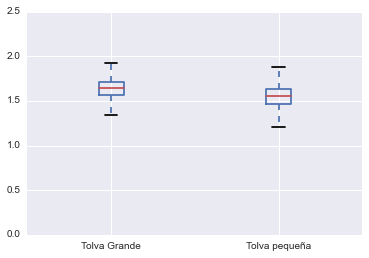
\includegraphics[width=0.8\textwidth]{images/producciones/22072015/output_6_1.png}
    \caption{Diagrama de cajas }
    \label{fig:22072015-boxplot}
\end{figure}

Como se ve en el diagrama de cajas, en el que se representa la distribución de los datos, los datos obtenidos en el ensayo con la tolva grande, son algo más estables, por lo tanto, podemos confirmar, que las medidas tomadas anteriormente para intentar mejorar la producción son acertadas, sin embargo, como se aprecia en el gráfico siguiente, se sigue teniendo una variación muy alta en el sistema, lo cual es un problema para intentar integrar un regulador del tipo PID. Por ello, se decide implementar un regulador experto para intentar controlar de forma más precisa el diámetro.


		%5
	\section{Regulador experto}
\label{sec:reg_expt}

Durante las producciones realizadas anteriormente, se ha notado que existe una relación entre la velocidad de tracción y el diámetro final del filamento, sin embargo, el sistema que se dispone carece de la robustez necesaria para poder trabajar con un regulador del tipo PID, en el que es necesario conocer de manera lo más exacta posible, la distribución de la planta con la que se trabaja.\\

Como se ha visto en los ensayos anteriores, la salida de filamento que proporciona el filastruder no es constante y en ocasiones, no está bien mezclada.

\begin{figure}[H]
    \centering
    \includegraphics[width=0.6\textwidth]{images/producciones/22072015/IMG_20150722_120959.jpg}
    \caption{Mezcla incorrecta de la filastruder}
    \label{fig:reg_mezcla}
\end{figure}

Por ello, se decide no usar un regulador PID e intentar implementar un regulador experto, el cual, imitará las acciones que un humano tomaría para resolver el problema. Este tipo de reguladores se basan en un conocimiento previamente adquirido por una persona, que ha trabajado con el sistema.\\

Para implementear este sistema, se definen una serie de reglas, en las que acotaremos los diámetros del filamento en regiones, y dependiendo, de si el diámetro crece o decrece, se actuará sobre la velocidad de tracción
\begin{figure}[H]
    \centering
    \includegraphics[width=0.5\textwidth]{images/producciones/11082015/Diagram1.png}
    \caption{Reglas a utilizar en el sistema experto}
    \label{fig:reg_reglas}
\end{figure}

Se realiza un bloque de programación que implemente esta filosifía y en función del diáemtro actual, y el diámetro anterior, se irá modificando la velocidad de tracción, para así variar el diámetro del filamento.\\

Una vez realiado el programa, se van a realizar varios ensayos con distintos parámetros para ver cómo influye el regulador.

\subsection{Ensayo 1}

Los datos con los que se realizaron el experimento fueron:

\begin{itemize}
	\item{Duración de experimento: 38 min}
	\item{Filamento extruido: 537 cm}
	\item{Granza de PLA mezcla: 70\% granza, 30\% pellets.}
	\item{Mezcla secada en horno 4 horas antes del ensayo.}
	\item{$T: 150ºC$}
	\item{$V_{min} tractora: 1.5 mm/s$}
	\item{$V_{max} tractora: 3.4 mm/s$}
	\item{Los incrementos de velocidades en las reglas del sistema experto son las mismas.}
\end{itemize}

Los resultados obtenidos son los siguientes:

\begin{table}[H]
	\centering
	\begin{tabular}{cc}
		                    & Diámetro X \\ \hline
		Medidas             & 1526       \\
		Media (mm)          & 1.72       \\
		Desviación estandar & 0.29       \\
		Mínimo (mm)         & 1.20       \\
		Máximo (mm)         & 2.56      
	\end{tabular}
	\caption{Datos obtenidos en el ensayo 1}
	\label{tab:resl_ens1}
\end{table}

Cómo vemos en la tabla \ref{tab:resl_ens1} la media del filamento conseguido es de $1.72 mm$, sin embargo, los valores límites de $1.65 mm$ y $1.85 mm$ han sido superados, por lo que el filamento que se ha extruido, no valdría en su totalidad para imprimir. Si representamos los datos obtenidos en una gráfica, podemos observar como hay una influencia del regulador. Las variaciones que hay en el diámetro, son no son tan pronunciadas como en el caso del funcionamiento en lazo abierto. \\

Con el gráfico de cajas, podemos ver que la distribución de los datos no es del todo homogena, teniendo una gran cantidad de los datos por encima de la media, sobre $1.96 mm$.

\begin{figure}[H]
    \centering
    \includegraphics[width=0.99\textwidth]{images/producciones/11082015/output_9_1.png}
    \caption{Datos graficados del ensayo 1 con regulador experto}
    \label{fig:reg_graf1}
\end{figure}

\begin{figure}[H]
    \centering
    \includegraphics[width=0.6\textwidth]{images/producciones/11082015/output_10_1.png}
    \caption{Diagrama de cajas del ensayo 1 con regulador experto}
    \label{fig:reg_cajas1}
\end{figure}

Como segunda aproximación que vamos a realizar será la de hacer mayores incrementos al subir la velocidad en los tramos que el diámetro se encuentre entre $1.80 mm$ y $1.75 mm$ haremos incrementos de velocidad mayor.

\subsection{Ensayo 2}

Los datos con los que se realizaron el experimento fueron:

\begin{itemize}
	\item{Duración de experimento: 30 min}
	\item{Filamento extruido: 435cm}
	\item{Granza de PLA mezcla: 70\% granza, 30\% pellets.}
	\item{Mezcla secada en horno 4 horas antes del ensayo.}
	\item{$T: 150ºC$}
	\item{$V_{min} tractora: 1.5 mm/s$}
	\item{$V_{max} tractora: 3.4 mm/s$}
	\item{Los incrementos de velocidades en las reglas del sistema experto son distintas:}
\end{itemize}

En este ensayo, se va a cambiar el incremento de velocidad, cuando el filamento esté entre una diámetro de $1.75 mm$ y $1.80 mm$ y tenga una tendencia de crecimiento. Se hará que en este caso, la velocidad se incremente más.\\

Los resultados obtenidos son los siguientes:

\begin{table}[H]
	\centering
	\begin{tabular}{cc}
		                    & Diámetro X \\ \hline
		Medidas             & 1114      \\
		Media (mm)          & 1.74       \\
		Desviación estandar & 0.26       \\
		Mínimo (mm)         & 1.02       \\
		Máximo (mm)         & 2.45      
	\end{tabular}
	\caption{Datos obtenidos en el ensayo 2}
	\label{tab:resl_ens2}
\end{table}

Con los cambios realizados, los datos ahora son algo más estables, y hemos conseguido aumentar la media del filamento a $1.74 mm$ estando dentro del margen de producción, sin embargo, los límites superior e inferior no son los adecuados, alejándose demasiado de lo deseado. Sin embargo en este caso, una gran parte del filamento podría llegar a ser re-aprovechado para imprimir.

\begin{figure}[H]
    \centering
    \includegraphics[width=0.99\textwidth]{images/producciones/12082015/output_9_e1.png}
    \caption{Datos graficados del ensayo 2 con regulador experto}
    \label{fig:reg_graf2}
\end{figure}

\begin{figure}[H]
    \centering
    \includegraphics[width=0.6\textwidth]{images/producciones/12082015/output_10_e1.png}
    \caption{Diagrama de cajas del ensayo 2 con regulador experto}
    \label{fig:reg_cajas2}
\end{figure}

Como tercera aproximación, vamos a modificar los incrementos de velocidades en los tramos en los que el filamento se encuentre entre  $1.70 mm$ y $1.80 mm$

\subsection{Ensayo 3}

Los datos con los que se realizaron el experimento fueron:

\begin{itemize}
	\item{Duración de experimento: 30min}
	\item{Filamento extruido: 425cm}
	\item{Granza de PLA mezcla: 70\% granza, 30\% pellets.}
	\item{Mezcla secada en horno 4 horas antes del ensayo.}
	\item{$T: 150ºC$}
	\item{$V_{min} tractora: 1.5 mm/s$}
	\item{$V_{max} tractora: 3.4 mm/s$}
	\item{Los incrementos de velocidades en las reglas del sistema experto son distintas:}
\end{itemize}

En este ensayo, se va a cambiar el incremento de velocidad, cuando el filamento esté entre una diámetro de $1.75 mm$ y $1.80 mm$ y sea cual sea la tendencia. Se hará que en este caso, la velocidad se incremente más.\\

Los resultados obtenidos son los siguientes:

\begin{table}[H]
	\centering
	\begin{tabular}{cc}
		                    & Diámetro X \\ \hline
		Medidas             & 1124      \\
		Media (mm)          & 1.66       \\
		Desviación estandar & 0.24       \\
		Mínimo (mm)         & 0.98       \\
		Máximo (mm)         & 2.60      
	\end{tabular}
	\caption{Datos obtenidos en el ensayo 3}
	\label{tab:resl_ens3}
\end{table}

Con esta tercera aproximación se ha conseguido estabilizar los datos y reducir la desviación estandar, sin embargo, la media del filamento y de la velocidad de tracción ha disminuido también. Por lo tanto, los cambios realizados no han sido satisfactorio

\begin{figure}[H]
    \centering
    \includegraphics[width=0.99\textwidth]{images/producciones/12082015/output_9_e2.png}
    \caption{Datos graficados del ensayo 3 con regulador experto}
    \label{fig:reg_graf3}
\end{figure}

\begin{figure}[H]
    \centering
    \includegraphics[width=0.6\textwidth]{images/producciones/12082015/output_10_e2.png}
    \caption{Diagrama de cajas del ensayo 3 con regulador experto}
    \label{fig:reg_cajas3}
\end{figure}

Como cuarta  aproximación, vamos a  modificar los incrementos en los que el diámetro se encuentra entre $1.70 mm$ y $1.80 mm$, en sentido de subida. En el sentido de bajada se mantendrá con incrementos de +1.\\

Se ha detectado también que el eje de giro de la tractora está algo suelto. Se va a apretar para el siguiente ensayo.\\

\subsection{Ensayo 4}

Los datos con los que se realizaron el experimento fueron:

\begin{itemize}
	\item{Duración de experimento: 30min}
	\item{Filamento extruido: 447cm}
	\item{Granza de PLA mezcla: 70\% granza, 30\% pellets.}
	\item{Mezcla secada en horno 4 horas antes del ensayo.}
	\item{$T: 150ºC$}
	\item{$V_{min} tractora: 1.5 mm/s$}
	\item{$V_{max} tractora: 3.4 mm/s$}
	\item{Los incrementos de velocidades en las reglas del sistema experto son distintas.}
\end{itemize}

 Los tramos entre $1.70 mm$ y $1.80mm$ en los que haya una tendencia a aumentar, se incrementará la velocidad, sin embargo cuando se tenga una tendencia a disminuir, se volverá a tener una incremento de velocidad de +1.\\

Los resultados obtenidos son los siguientes:

\begin{table}[H]
	\centering
	\begin{tabular}{cc}
		                    & Diámetro X \\ \hline
		Medidas             & 1125      \\
		Media (mm)          & 1.71       \\
		Desviación estandar & 0.23       \\
		Mínimo (mm)         & 1.01       \\
		Máximo (mm)         & 2.30      
	\end{tabular}
	\caption{Datos obtenidos en el ensayo 4}
	\label{tab:resl_ens4}
\end{table}

Con esta tercera aproximación se ha conseguido estabilizar los datos y reducir la desviación estandar, sin embargo, la media del filamento y de la velocidad de tracción ha disminuido también. Por lo tanto, los cambios realizados no han sido satisfactorio

\begin{figure}[H]
    \centering
    \includegraphics[width=0.99\textwidth]{images/producciones/13082015/output_9_e1.png}
    \caption{Datos graficados del ensayo 4 con regulador experto}
    \label{fig:reg_graf4}
\end{figure}

\begin{figure}[H]
    \centering
    \includegraphics[width=0.6\textwidth]{images/producciones/13082015/output_10_e1.png}
    \caption{Diagrama de cajas del ensayo 4 con regulador experto}
    \label{fig:reg_cajas4}
\end{figure}

Como quinta  aproximación, vamos a  modificar los rangos de velocidades de la tractora. Vamos a pasar a unas velocidades de $1.5RPM$ a $5.3RPM$ \\

\subsection{Ensayo 5}

Los datos con los que se realizaron el experimento fueron:

\begin{itemize}
	\item{Duración de experimento: 20min}
	\item{Filamento extruido: 314cm}
	\item{Granza de PLA mezcla: 70\% granza, 30\% pellets.}
	\item{Mezcla secada en horno 4 horas antes del ensayo.}
	\item{$T: 150ºC$}
	\item{$V_{min} tractora: 1.5 mm/s$}
	\item{$V_{max} tractora: 5.3 mm/s$}
	\item{Los incrementos de velocidades en las reglas del sistema experto son distintas.}
\end{itemize}

Este experimento sólo dura 20min, debido a que durante la realización del mismo, se percibe que no aporta ninguna mejora, añadiendo más inestabilidad a la medidas.\\

Los resultados obtenidos son los siguientes:

\begin{table}[H]
	\centering
	\begin{tabular}{cc}
		                    & Diámetro X \\ \hline
		Medidas             & 750      \\
		Media (mm)          & 1.43       \\
		Desviación estandar & 0.36       \\
		Mínimo (mm)         & 0.00       \\
		Máximo (mm)         & 2.31      
	\end{tabular}
	\caption{Datos obtenidos en el ensayo 5}
	\label{tab:resl_ens5}
\end{table}

\begin{figure}[H]
    \centering
    \includegraphics[width=0.99\textwidth]{images/producciones/13082015/output_9_e2.png}
    \caption{Datos graficados del ensayo 5 con regulador experto}
    \label{fig:reg_graf5}
\end{figure}

\begin{figure}[H]
    \centering
    \includegraphics[width=0.6\textwidth]{images/producciones/13082015/output_10_e2.png}
    \caption{Diagrama de cajas del ensayo 5 con regulador experto}
    \label{fig:reg_cajas5}
\end{figure}

Aumentando la velocidad se ha conseguido que disminuya el valor máximo, sin embargo ha disminuido el valor mínimo. Para la siguiente iteracción, se va a volver a las velocidades de $1.5RPM$ - $3.4RPM$ y se van a añadir más reglas con unos incrementos de velocidades menores, para evitar saturar la velocidad de traccción tanto a nivel alto como nivel bajo.

\subsection{Ensayo 6}

Los datos con los que se realizaron el experimento fueron:

\begin{itemize}
	\item{Duración de experimento: 30min}
	\item{Filamento extruido: 453cm}
	\item{Granza de PLA mezcla: 70\% granza, 30\% pellets.}
	\item{Mezcla secada en horno 4 horas antes del ensayo.}
	\item{$T: 150ºC$}
	\item{$V_{min} tractora: 1.5 mm/s$}
	\item{$V_{max} tractora: 3.4 mm/s$}
	\item{Los incrementos de velocidades en las reglas del sistema experto son distintas.}
\end{itemize}

 Los tramos entre $1.70 mm$ y $1.80mm$ en los que haya una tendencia a aumentar, se incrementará la velocidad, sin embargo cuando se tenga una tendencia a disminuir, se tendrá una incremento de velocidad de +1.\\

Los resultados obtenidos son los siguientes:

\begin{table}[H]
	\centering
	\begin{tabular}{cc}
		                    & Diámetro X \\ \hline
		Medidas             & 1087      \\
		Media (mm)          & 1.71       \\
		Desviación estandar & 0.26       \\
		Mínimo (mm)         & 1.05       \\
		Máximo (mm)         & 2.44      
	\end{tabular}
	\caption{Datos obtenidos en el ensayo 6}
	\label{tab:resl_ens6}
\end{table}

Con esta tercera aproximación se ha conseguido estabilizar los datos y reducir la desviación estandar, sin embargo, la media del filamento y de la velocidad de tracción ha disminuido también. Por lo tanto, los cambios realizados no han sido satisfactorio

\begin{figure}[H]
    \centering
    \includegraphics[width=0.99\textwidth]{images/producciones/13082015/output_9_e3.png}
    \caption{Datos graficados del ensayo 6 con regulador experto}
    \label{fig:reg_graf6}
\end{figure}

\begin{figure}[H]
    \centering
    \includegraphics[width=0.6\textwidth]{images/producciones/13082015/output_10_e3.png}
    \caption{Diagrama de cajas del ensayo 6 con regulador experto}
    \label{fig:reg_cajas6}
\end{figure}

\subsection{Conclusiones}

Después de realizar los seis experimentos, estos son los resultados en cada uno de ellos.\\

\begin{table}[H]
	\centering
	\begin{tabular}{lccccccc}
		                    &Lazo Abierto     & Ensayo 1 & Ensayo 2 & Ensayo 3 & Ensayo 4 & Ensayo 5 & Ensayo 6 \\ \hline
		Medidas             &     203         & 1526     & 1114     & 1124     & 1125     & 750      & 1087     \\
		Media (mm)          &	1.59		 & 1.72     & 1.74     & 1.66     & 1.71     & 1.43     & 1.71     \\
		Desviación estandar &	0.25		 & 0.29     & 0.26     & 0.24     & 0.23     & 0.36     & 0.26     \\
		min(mm)             &	1.08		 & 1.20     & 1.02     & 0.98     & 1.01     & 0        & 1.05     \\
		max(mm)             &	2.19		 & 2.56     & 2.45     & 2.60     & 2.30     & 2.31     & 2.44    
	\end{tabular}
	\caption{Tabla comparativa de los resultados obtenidos}
	\label{tab:compara_results}
\end{table}


Como podemos comprobar, hemos conseguido tener un diámetro, cuyo valor medio está dentro de los márgenes de teolerancia, sin embargo, los valores máximos y mínimos no cumplen los requisitos. Esto es debido a que el filamento no sale de manera constante de la extrusora y por ello, el control del mismo, se hace más complicado si cabe. Sin embaego, hemos podido comprobar como el regulador que hemos implementado aplica una cierta mejora respecto al extrusor en lazo abierto.\\

Tomando como los datos obtenidos en el ensayo 4, como unos válidos para producción, vamos a pasar a compararlos con los datos obtenidos de dos fabricantes distintos de filamento, para ver posibles similitudes entre ellos.

\begin{table}[H]
	\centering
	\begin{tabular}{ccccccc}
		                    & BQ & FormFutura & Filastruder \\ \hline
		Medidas             & 291     &291    & 291      \\
		Media (mm)          & 1.75     & 1.70     & 1.74      \\
		Desviación estandar & 0.01     & 0.05     & 0.21      \\
		min(mm)             & 1.67     & 1.64     & 1.01      \\
		max(mm)             & 1.77     & 1.71     & 2.14     
	\end{tabular}
	\caption{Tabla comparativa de los resultados obtenidos}
	\label{tab:compara_results}
\end{table}

\begin{figure}[H]
    \centering
    \includegraphics[width=0.99\textwidth]{images/producciones/conclusiones/output_8_1.png}
    \caption{Comparativa filamentos distintos fabricantes}
    \label{fig:concl_graf5}
\end{figure}

\begin{figure}[H]
    \centering
    \includegraphics[width=0.6\textwidth]{images/producciones/conclusiones/output_9_1.png}
    \caption{Diagrama de cajas con diámetros de distintos fabricantes}
    \label{fig:concl_cajas5}
\end{figure}

Como podemos observar en los datos, el diámetro de los filamentos que proporcionan empresas como bq y formfutura, tienen unos valores mucho más estables que los nuestros. Lo cual es normal debido a la maquinaría y condiciones de trabajo que se han realizado en los experimentos. No obstante, teniendo en cuenta el material con el que se han realizado todos los ensayos podemos afirmar que el regulador implementado supone una mejorar en el diámetro final del filamento.		%5
	\chapter{Conclusiones y trabajos futuros}
\label{cap:conclus}

En este capítulo se discutirá el trabajo realizado durante el proyecto, así como el trabajo que queda por realizar desde la división de automatización y materiales de BQ a medio-largo plazo.

\section{Cumplimiento de los objetivos}

Al finalizar el proyecto, nos encontramos con un sistema capaz de obtener los datos más importantes que caracterizan la calidad de un filamento. Con estos datos podremos trabajar a posteriori y tener una trazabilidad del filamento completa en caso de que se reciba alguna reclamación por parte de los clientes.\\

En el momento de plantear la idea de este proyecto, BQ tiene acceso a tres líneas de extrusión de filamento,  pudiendo instalar el sistema en una de ellas. Sin embargo en el momento de realizar la puesta en marcha, no se pude ceder esa línea debido a temas de planificación en la producción de filamento.\\

Para solucionar esto se adquiere una extrusora de laboratorio en la cual también es válido el sistema de adquisición de datos, pero hay retrasos en la entrega y no hacen posible disponer de ella antes de la entrega de este proyecto.\\

En el departamento de Innovación y Robótica, se tiene una maqueta de una extrusora casera la cual es totalmente válida para demostrar el funcionamiento de nuestro sistema. A pesar de que la extrusora produce plástico de poca calidad, es válida para comprobar nuestro sistema de control de calidad.\\

Por tanto, al terminar  el proyecto, podemos afirmar que se han acometido todas las fases del proceso de fabricación del PLA. Al tener la extrusora casera, se han fabricado las herramientas necesarias para generar pellets de filamento reciclado (peletizadora) y poder comprobar su correcto uso a la hora de extruirlo.

\section{Líneas de trabajo abiertas en BQ a raiz de este trabajo final de grado}

Durante la realización del proyecto, en la división de automatización y materiales, se ha usado el sistema de adquisición de datos para realizar un estudio de la degradación del PLA con el paso del tiempo. Después de recibir varias reclamaciones de los clientes se está investigando sobre cómo puede afectar el correcto almacenamiento de una bobina de PLA en el diámetro del mismo. Para ello, el estudio consta de las siguientes partes:

\begin{itemize}
	\item{Medir el diámetro de una longitud determinada de una bobina recién sacada de su embalaje}
	\item{Someter al filamento a diversas pruebas. Las cuales consiste en almacenar el filamento en unas condiciones de temperatura extremas, tanto en un congelador para enfriar, así como en un horno a una temperatura alta.}
	\item{Volver a medir el diámetro y estudiar los cambios}
\end{itemize}

Gracias a esto, se están empezando a caracterizar estos problemas y obtener una solución rápida al cliente en caso de que los síntomas sean parecidos.\\

Así mismo, y algo que era un trabajo a realizar en el futuro en el departamento, se ha diseñado un sistema capaz de reciclar las bobinas de filamento que no eran útiles para un uso final en impresoras 3D y cómo hemos visto, el material reciclado obtenido es completamente válido para volver a realizar filamento.\\

Este proyecto de adquisición de datos no termina con la defensa de esta memoria. Desde BQ se va a seguir mejorando e incluyendo nuevas características que harán más versatil el sistema.

\section{Mejoras}
Derivado a estos trabajos, se requieren las siguientes mejoras en las que se va a empezar a trabajar lo antes posible:

\begin{itemize}
	\item{Almacenamiento de la información en una base datos MYSQL. En lugar de almacenar la información en una tarjeta SD, se plantea almacenar toda la información en un servidor para poder realizar informes en tiempo real de la producción.}
	\item{Incorporar una impresora para generar pegatinas con códigos QR. De tal manera, si el sistema determina que el filamento extruido no cumple unos requisitos mínimos, automaticamente al ver la pegatina, se sepa si esa bobina pasa el control de calidad.}
	\item{En el año 2016 se tiene previsión de adquirir varias lineas de extrusión por tanto y gracias a que nuestro sistema es escalable en prestacións, se puede realizar un sistema de supervisión superior en el que se tenga acceso del estado de la fábrica en la que se encuentre cada línea de extrusión y su información. En este caso, la información ya no se almacenaria en el sistema local, si no que haría falta un sistema de tratamiento de datos online.}

\end{itemize}

\section{Valoración final}

El resultado final del proyecto ha sido satisfactorio, presenteando un sistema versatil y capaz de solucionar el problema que se plantea al inicio. A raiz de la elaboración del proyecto, han surgido nuevos problemas los cuales se han afrontado como pequeños proyectos necesarios para la consecución del objetivo principal.\\

Estos proyectos han sido minuciosamente documentados puesto que pueden ser aplicados en trabajos de otra índole que no sea la de extruir filamento. Por este motivo esta información se ha añadido a los anexos para que de este modo, quede constancia del trabajo desarrollado y alguién en el futuro pueda serle de utilidad.\\

La realización de este trabajo final de grado ha llevado consigo el aporte de nuevos conocimientos en diversas materias como son: ingeniería mecánica, ingeniería de materiales, análisis de datos, trabajo en grupo y gestión de proyectos.	%6
	%%%%%%% Apéndices
	%%%%%%%%%%%%%%%%%
	\begin{appendix}
		\appendixpage
		\chapter{Presupuesto}
\label{ane:presupuesto}

\section{Presupuesto detallado}

\begin{longtable}{l c p{7cm} c r r}
    \hline
    Código & Unidad & Descripción  & Cantidad & Precio(\euro) & Total(\euro)  \\ \hline \hline 
    
    %%%% Sistema de adquisicón %%%%%%%%%%%%%%%%%%%%%%%%%%%%%%%%%%%%%%%%%%%%%%%%%
    1 & unidad & \textbf{Sistema de adquisición} & 1 & \multicolumn{1}{r}{} & 947.50 \\ \hline 
    
    %%% Armario %%%%%%%%%%%%%%%%%%%%%%%%%%
    1.1 & unidad & \textbf{Armario} & 1 & 156.80 & 156.80 \\ \hline  
    
    1.1.1 & unidad & \textbf{Caja de pared} \newline \small Caja de policarbonato rellena de fibra de vidrio, resistente de alto impacto, que ofrece una alternativa viable y rentable a las cajas de acero de montaje en la pared. El material utilizado no tiene halógenos y está probado frente a llamas a UL94-V2 (autoextinguible).& 1 & 77.02 & 77.02  \\ \hline

    1.1.2 & unidad & \textbf{Placa de montaje} \newline \small Placa de acero galvanizado, espesor de chapa 1,5 mm. Usado para realizar el montaje de los elementos en ella y facilitar la instalación. & 1 & 7.22 & 7.22  \\ \hline

    1.1.3 & unidad & \textbf{Casquillos y prensaestopas} \newline \small Prensaestopas con apriete antivibración.
    Junta tórica de neopreno. & 2 & 7.13 & 14.26  \\ \hline

    1.1.4 & unidad & \textbf{Bornas de conexión} \newline \small bornas con abrazadera roscada. Diseñados para montarse en carriles DIN de perfil en U utilizando un perfil asimétrico único que añade visibilidad desde cualquier dirección y evita errores de montaje inverso. Fáciles de instalar con encaje a presión positivo y construidos con material pirorretardante con reborde. & 20 & 0.602 & 12.04  \\ \hline
    
    1.1.5 & unidad & \textbf{Bornas de conexión a tierra} \newline \small bornas con abrazadera roscada. Diseñados para montarse en carriles DIN de perfil en U utilizando un perfil asimétrico único que añade visibilidad desde cualquier dirección y evita errores de montaje inverso. Fáciles de instalar con encaje a presión positivo y construidos con material pirorretardante con reborde. & 1 & 2.00 & 2.00  \\ \hline
    
    1.1.6 & unidad & \textbf{Embellecedor de bornas de conexión} \newline \small Tapas para colocar al final de una hilera de bornas. & 1 & 0.42 & 0.42  \\ \hline 
    
    1.1.7 & unidad & \textbf{Fuente de alimentación para plc} \newline \small Fuente para plc MDR-40-24 Provee una tensión continua de 24V,y una corriente de salida de hasta 1.7A. & 1 & 18.00 & 18.00\\ \hline 

    1.1.8 & unidad & \textbf{Puntera hueca de crimpado} \newline \small Puntera de crimpado de gama de colores francesa fabricadas de cobre estañado brillante con fundas aislantes de polipropileno que aceptan cables 2491X y trinominales. Esta gama de punteras de crimpado de gama de colores francesa proporciona una terminación limpia para cables multifilares y reduce la posibilidad de cortocircuitos en terminales adyacentes y garantizan una conexión positiva que se utiliza con bloques de terminales y terminales cautivos. & 74 & 0.074 & 5.47  \\ \hline

    1.1.9 & metros & \textbf{Cable multifilar de color azul} Alambre trenzado, para cableado flexible en armarios eléctricos, equipos y aplicaciones de iluminación. También para uso sobre y bajo yeso para el cableado de la señal. \newline \small & 2 & 0.27 & 0.54  \\ \hline

    1.1.10 & metros & \textbf{Cable multifilar de color negro} Alambre trenzado, para cableado flexible en armarios eléctricos, equipos y aplicaciones de iluminación. También para uso sobre y bajo yeso para el cableado de la señal. \newline \small & 2 & 0.27 & 0.54  \\ \hline
   
    1.1.11 & metros & \textbf{Cable multifilar de color verde y amarillo} Alambre trenzado, para cableado flexible en armarios eléctricos, equipos y aplicaciones de iluminación. También para uso sobre y bajo yeso para el cableado de la señal. \newline \small & 2 & 0.27 & 0.54  \\ \hline

    1.1.12 & unidad & \textbf{Carril DIN} \newline \small Los carriles DIN están fabricados en acero laminado en frío con recubrimiento de zinc y pasivado. El espesor del recubrimiento es de un mínimo de 8 micrones. Todos los carriles DIN cumplen las normas vigentes BS, DIN y CENELEC. & 2 & 3.81  &  7.62\\ \hline

    1.13 & metros & \textbf{Manguera de hilo de 6 polos de 0.22} \newline \small Manguera de cable con 6 hilos para instalaciónes de tensión baja, para instalaciones remotas, para transferir señales, para transferir datos. & 0.5 & 0.725  &  0.362\\ \hline
    
    1.14 & unidad & \textbf{Interruptor automático de dos polos.} \newline \small Interruptor automático Solera 3SB1-63H1-C10 de dos polos residencial y terciario. 10A, curva C. 6kA. & 1 & 5.60  & 5.60 \\ \hline

    1.14 & unidad & \textbf{Interruptor automático de un polo.} \newline \small Interruptor automático Solera 3SB1-63H1-C16 de dun polos residencial y terciario. 10A, curva C. 6kA. & 1 & 5.60  & 5.60 \\ \hline

    &&&& Subtotal: & 156.80\\
     \\~\\  \hline


    %%% Automáta %%%%%%%%%%%%%%%%%%%%%%%%%%
    1.2 & unidad & \textbf{Automáta programable industrial} & 1 & 790.70 & 790.70 \\ \hline

    1.2.1 & unidad & \textbf{CPU AC500-eco} \newline \small PM564-RP-ETH CPU AC500-eCo,128kB,6DI/6DO-R/2AI/1AO, 24VDC. ETH y WEBSERVER. PLC compacto y modular con 128kB de memoria de programa (512kB para la PM556-TP-ETH). Tiempos de ciclo mínimo para 1 instrucción: bit: $0.08\mu s$, palabra:$ 0.1\mu s$ y coma flotante: $1.2\mu s$. Potente programación según IEC 61131-3 mediante 5 lenguajes: LD, ST, FBD, IL y SFC. Posibilidad de expansión con hasta 10 módulos de E/S S500 y/o S500-eCo. Cableado muy fácil de los módulos de E/S S500-eCo mediante bloques de terminales desenchufables de tornillo o resorte con conexión frontal o lateral.& 1 & 415.14 & 415.14  \\ \hline
    
    1.2.2 & unidad & \textbf{Módulo de entradas analógicas} \newline \small AI562 Módulo S500-eCo. Módulo de expansión de entradas analógicas. Dispone de dos entradas analógicas par PT100/1000, Ni100/1000 o Resist. 150/300. & 1 & 247.66 & 247.66 \\ \hline
    
    1.2.3 & unidad & \textbf{SD Memory Card 512 MB} \newline \small MC502 SD Memory Card 512 MB. Tarjeta de expansión SD. & 1 & 79.17 & 79.17 \\ \hline
    
    1.2.4 & unidad & \textbf{Adaptador para SD memory card} \newline \small MC503 Adaptador para tarjeta SD de memoria AC500-eCo. Adaptador necesario para poder incluir una tarjeta SD en la cpu del automáta programable. & 1 & 31.47 & 31.47 \\ \hline
    
    1.2.5 & unidad & \textbf{Conector 9 polos para módulos S500-eCo} \newline \small TA565-9 Conector 9 polos para módulos S500-eCo, resorte / frontal.Dispositivo necesario para poder cablear las distitnas entradas salidas de la CPU. & 1 & 5.08 & 5.08 \\ \hline
    
    1.2.6 & unidad & \textbf{Conector 11 polos para módulos S500-eCo} \newline \small TA565-11 Conector 11 polos para módulos S500-eCo, resorte / frontal.Dispositivo necesario para poder cablear las distitnas entradas salidas de la CPU. & 1 & 6.08 & 6.08 \\ \hline
    &&&& Subtotal: &790.70\\
     \\~\\  \hline
    
    Código & Unidad & Descripción  & Cantidad & Precio(\euro) & Total(\euro)  \\ \hline \hline 
    %%%% Maqueta %%%%%%%%%%%%%%%%%%%%%%%%%%%%%%%%%%%%%%%%%%%%%%%%%
    2 & unidad & \textbf{Maqueta extrusora casera} & 1 & \multicolumn{1}{r}{} & 132.08 \\ \hline

    2.1 & unidad & \textbf{Fuente de alimentación 12V y 30A}. Fuente de alimentación con una tensión de 12v de tensión continua y una salida máxima de hasta 30A. & 1 & 60.00 & 60.00 \\ \hline
    
    2.2 & unidad & \textbf{Relé} Relé universal DPDT 8Amps 24VAC. & 3 & 4.07 & 12.21 \\ \hline
    
    2.3 & unidad & \textbf{Carcasas y utillaje de relés} Carcasa con montaje DIN para reles. INcluye terminales con tornillos para facilitar la conexión de cables al relé. & 3 &  5.16 & 15.48 \\ \hline
    
    2.4 & unidad & \textbf{Interruptor automático de dos polos.} \newline \small Interruptor automático Solera 3SB1-63H1-C10 de dos polos residencial y terciario. 10A, curva C. 6kA. & 1 & 5.60  & 5.60 \\ \hline

    2.5 & metros & \textbf{Cable multifilar de color azul} \newline \small Alambre trenzado, para cableado flexible en armarios eléctricos, equipos y aplicaciones de iluminación. También para uso sobre y bajo yeso para el cableado de la señal. \newline \small & 1 & 0.27 & 0.27 \\ \hline

    2.6 & metros & \textbf{Cable multifilar de color negro} \newline \small Alambre trenzado, para cableado flexible en armarios eléctricos, equipos y aplicaciones de iluminación. También para uso sobre y bajo yeso para el cableado de la señal. \newline \small & 1 & 0.27 & 0.27 \\ \hline
   
    2.7 & metros & \textbf{Cable multifilar de color verde y amarillo} \newline \small Alambre trenzado, para cableado flexible en armarios eléctricos, equipos y aplicaciones de iluminación. También para uso sobre y bajo yeso para el cableado de la señal. \newline \small & 1 & 0.27 & 0.27 \\ \hline

    2.8 & unidad & \textbf{Carril DIN} \newline \small Los carriles DIN están fabricados en acero laminado en frío con recubrimiento de zinc y pasivado. El espesor del recubrimiento es de un mínimo de 8 micrones. Todos los carriles DIN cumplen las normas vigentes BS, DIN y CENELEC. & 2 & 3.81  &  7.62\\ \hline

    2.9 & unidad & \textbf{Sensor de diámetro} \newline \small Sensor de diámetro meediante sensor CCD. Con una resolución de hasta 0.01 mm. Es capaz de medir cilindros comprendidos entre 0.9 mm y 3mm. & 2 & 14.5 & 29\\ \hline
    
    2.10 & unidad & \textbf{Piezas impresas} \newline \small Distintas piezas impresas realizadas para suplir ciertas necesidades a la hora de la ejecución del proyecto & 1 & 8.5 & 8.5\\ \hline
  
    2.11 & unidad & \textbf{Bornas de conexión} \newline \small bornas con abrazadera roscada. Diseñados para montarse en carriles DIN de perfil en U utilizando un perfil asimétrico único que añade visibilidad desde cualquier dirección y evita errores de montaje inverso. Fáciles de instalar con encaje a presión positivo y construidos con material pirorretardante con reborde. & 12 & 0.60 & 7.20  \\ \hline
    
    &&&& Subtotal: &132.08\\

     \\~\\  \hline
     \pagebreak
    Código & Unidad & Descripción  & Cantidad & Precio(\euro) & Total(\euro)  \\ \hline \hline \hline \hline
    %%%% Software %%%%%%%%%%%%%%%%%%%%%%%%%%%%%%%%%%%%%%%%%%%%%%%%%%%%%
    3 & unidad & \textbf{Software} & 1 & \multicolumn{1}{r}{} & 140..00 \\ \hline
    3.1 & horas & \textbf{Tiempo de trabajo programación} & 70 & 20.00 & 140.00 \\ \hline  
    
    \\~\\ \hline
    
    Código & Unidad & Descripción  & Cantidad & Precio(\euro) & Total(\euro)  \\ \hline \hline \hline \hline
    %%%% Research %%%%%%%%%%%%%%%%%%%%%%%%%%%%%%%%%%%%%%%%%%%%%%%%%%%%%
    4 & unidad & \textbf{Costes de desarrollo} & 1 & \multicolumn{1}{r}{} & 6,200.00 \\ \hline
    4.1 & horas & \textbf{Tiempo de trabajo del desarrollo} & 310 & 20.00 & 6,200.00 \\ \hline  
   
\end{longtable}

\newpage
\section{Resumen del presupuesto}

\begin{center}
%\hspace*{-3cm}
    \begin{tabular}{ | l || p{9cm}  l | r | r |}
    \hline
    \textbf{Código} & \multicolumn{1}{l}{\textbf{Descripción}} &  & \textbf{Coste (\euro)}  & \textbf{\% del coste total} \\ \hline \hline
    
    \textbf{1} & Sistema de adquisición &  & 947.50 & 12.77 \\ \hline
    
	\textbf{2} & Maqueta extrusora casera &  & 132.08& 1.78 \\ \hline

	\textbf{3} & Software &  & 140.00 & 1.88 \\ \hline 

    \textbf{4} & Costes de desarrollo &  & 6,200.00 & 83.57\\ \hline 
	
	\multicolumn{1}{r}{} & & \textbf{Total} & 7,419.08 & 100\\  \cline{4-5}
    	
	
\end{tabular}
\end{center}
		\chapter{Diagram Gantt}
\label{ane:gant}

%\includepdf[pages=-]{gantt.pdf}
\begin{figure}[!ht]
    \centering
    \includegraphics[width=0.99\textwidth]{images/gantt.png}
    \caption[Aproximación de una pieza con fabricación aditiva.]{Aproximación de una pieza con fabricación aditiva. A la izquierda podemos observar la forma}
    \label{fig:gantt}
\end{figure}
		\input{PLC}
		\chapter{Esquemas eléctricos}
\label{ane:esquemas_electricos}
		\includepdf[pages=-]{00Armario.pdf}
		\includepdf[pages=-]{00Filastruder.pdf}
		\chapter{Montaje Filastruder}
\label{ane:filastruder}

La filastruder va a ir instalada sobre una plancha de madera en la que también se cablean los elementos usados en el proyecto:

   	\begin{figure}[H]
            \centering
            \includegraphics[width=0.6\textwidth]{images/filaextruder/IMG_20150313_114401.jpg}
            \caption{Se ancla la extructura a la base}
            \label{fig:fila_montaje1}
    \end{figure}
    \begin{figure}[H]
            \centering
            \includegraphics[width=0.6\textwidth]{images/filaextruder/IMG_20150324_175818.jpg}
            \caption{Calefactor en la alimentación y cañon}
            \label{fig:fila_montaje2}
    \end{figure}
    \begin{figure}[H]
            \centering
            \includegraphics[width=0.6\textwidth]{images/filaextruder/IMG_20150325_145634.jpg}
            \caption{Sensor PT100 de temperatura}
            \label{fig:fila_montaje3}
    \end{figure}

Una vez instalados los cartuchos y las sondas de temperatura en la filastruder, se pasa a aislar el cañón para que la disipación de calor al exterior no sea elevada y poder mantener una temperatura constante.

    \begin{figure}[H]
            \centering
            \includegraphics[width=0.4\textwidth]{images/filaextruder/IMG_20150814_132929.jpg}
            \caption{Filastruder montado}
            \label{fig:fila_montaje4}
    \end{figure}

El siguiente paso es cablear todas las señales a un armario que instalaremos en la propia maqueta en el espacio reservado para ello, este armario estará conectado al armario del PLC para poder realizar el control de la maqueta:

    \begin{itemize}
    	\item Sondas de temperatura.
    	\item Reles para controlar las resistencias de potencia y el motor del husillo.
    \end{itemize}

El circuito eléctrico a cablear está indicado en el Anexo \ref{ane:esquemas_electricos}.

    \begin{figure}[H]
            \centering
            \includegraphics[width=0.5\textwidth]{images/maqueta/IMG_20150324_162200.jpg}
            \caption{Presentación de los componentes en el lugar adecuado.}
            \label{fig:maque_montaje5}
    \end{figure}
    \begin{figure}[H]
            \centering
            \includegraphics[width=0.5\textwidth]{images/maqueta/IMG_20150324_162705.jpg}
            \caption{Atornillamos las canaletas y guias a la madera.}
            \label{fig:maque_montaje6}
    \end{figure}
    \begin{figure}[H]
            \centering
            \includegraphics[width=0.5\textwidth]{images/maqueta/IMG_20150324_173716.jpg}
            \caption{Cableamos los componentes según los esquemas.}
            \label{fig:maque_montaje7}
    \end{figure}
    \begin{figure}[H]
            \centering
            \includegraphics[width=0.5\textwidth]{images/maqueta/IMG_20150331_125243.jpg}
            \caption{Aspecto final cuadro eléctrico maqueta.}
            \label{fig:maque_montaje8}
    \end{figure}
		\section{Producciones}
\label{sec:producciones}

\subsection{Peletizadora}
\label{sec:peletizadora}

Algo que no se tuvo en cuenta al establecer los objetivos del proyecto, fue el tener disponibilidad de pellets de PLA, ya que en ese momento, los pellets no los proporcionarían en la fábrica de Huesca para poder hacer las pruebas de la puesta en marcha. Por ello, se investiga en la posibilidad de reciclar bobinas defectuosas que no son útiles para imprimir en una impresora 3D ocasionando averias y en la actualidad son mermas que se tiene en la producción de la fábrica de Huesca.

    \begin{figure}[H]
            \centering
            \includegraphics[width=0.6\textwidth]{images/peletizadora/Diagram.png}
            \caption{Proceso para conseguir pellets}
            \label{fig:peletizadora_diagram}
    \end{figure}

Una vez que la filastruder está operativa, se peletizan a mano unos metros de filamento negro y comprobamos que al menos somos capaces de extruir los pellets reciclados. Se continua con la línea de investigación del reciclado de bobina as al comprobar la viabilidad del proceso. Sin embargo, cada bobina de filamento de 1Kg de peso son 350M por lo que peletizar una bobina a mano, conllevaría mucho tiempo y trabajo, por lo que se descarta la opción y se pasa a diseñar una máquina capaz de peletizar bobinas de forma automática. La máquina que diseñemos debe ser capaz de realizar el siguiente proceso:

    \begin{figure}[H]
            \centering
            \includegraphics[width=0.6\textwidth]{images/peletizadora/Diagram2.png}
            \caption{Proceso funcionamiento peletizadora}
            \label{fig:peletizadora_diagram2}
    \end{figure}

Por tanto, debe tener al menos dos partes diferenciadas:

\begin{itemize}
		\item{\textbf{Unidad Tractora:} Mecanismo capaz de arrastrar el filamento hacía la unidad de corte.}
		\item{\textbf{Cuchillas de corte:} Mecanismo capaz de ejercer la fuerza necesaria para cortar el filamento.}
\end{itemize}

Para controlar toda la máquina se decide usar una placa arduino Mega que se tiene disponible en el departamento, con la que seremos capaz de controlarlo. Para la fabricación de la máquina, se usarán impresoras 3D, con lo que el prototipado será más rápido, ya que se tiene acceso a ellas dentro del departamento. Con las herramientas disponibles se inicia el diseño de la máquina.\\

Para la unidad tractora, se deciden usar dos motores paso a paso con un eje de giro recubierto de una goma, que cogerá el filamento y lo arrastrará. Usando la herramienta Inventor, se hace un primer diseño de la posible solución.

    \begin{figure}[H]
            \centering
            \includegraphics[width=0.6\textwidth]{images/peletizadora/unidadtractora.png}
            \caption{Diseño de la unidad tractora}
            \label{fig:peletizadora_tractora}
    \end{figure}

Los ejes, deberán ir recubiertos de goma de neopreno, para que puedan arrastrar del filamento. Se eligen motores paso a paso, debido a:

\begin{itemize}
	\item{Fáciles de programar.}
	\item{Fáciles de controlar en velocidad.}
	\item{Gran fuerza neta en el eje.}
\end{itemize}

Aunque el mecanismo es capaz de tirar del filamento bobinado, es necesario que se le guíe para que el corte sea siempre en la misma posición, por tanto, se diseña una guía para que la salida del filamento sea siempre por el mismo sitio, a la pieza impresa, se le pondrá una plancha de metal para que al realizar el corte, el filamento se apoye sobre ella y se ejerza más fuerza a cizalla. Además, deberá tener forma de embudo, para que la entrada del filamento sea lo más amplia posible y el final sea un único cilindro de un tamaño similar al del diámetro de filamento:

    \begin{figure}[H]
            \centering
            \includegraphics[width=0.4\textwidth]{images/peletizadora/guia.png}
            \caption{Diseño de guía de filamento}
            \label{fig:peletizadora_guia}
    \end{figure}

El diseño final de la unidad tractora se ve a continuación:

    \begin{figure}[H]
            \centering
            \includegraphics[width=0.5\textwidth]{images/peletizadora/conjunto_tractora.png}
            \caption{Conjunto tractora completo}
            \label{fig:peletizadora_conjunto}
    \end{figure}

Con este conjunto, garantizamos que el desbobinado del filamento sea correcto, aparte, seremos capaces de regular la velocidad de tracción de forma controlada. El siguiente paso a realizar será el diseño de las cuchillas de corte.\\

Como unidad motriz de las cuchillas de corte, se elige un taladro con fuerza ajustable, en la boca del mismo, se acoplará un eje con las cuchillas. Como primera idea, se piensa en un diseño con un molino a cuatro ejes, donde en cada uno de ellos irá una cuchilla, de esta manera, por cada giro se podrán realizar cuatro cortes.

    \begin{figure}[H]
            \centering
            \includegraphics[width=0.4\textwidth]{images/peletizadora/aspas.png}
            \caption{Diseño de las aspas}
            \label{fig:peletizadora_aspas}
    \end{figure}

El conjunto de las aspas, irán instaladas sobre dos pilares, que harán de eje de giro al taladro, a su vez, se instalará una rampa de salida, para que los pellets vayan cayendo por ella, por último, para tapar todas las cuchillas y añadir seguridad al mecanismo, se incorpora una tapa que hará que las cuchillas no sean accesibles.


    \begin{figure}[H]
            \centering
            \includegraphics[width=0.4\textwidth]{images/peletizadora/corte.png}
            \caption{Mecanismo de corte}
            \label{fig:peletizadora_corte}
    \end{figure}

Una vez impresas todas las piezas y realizado el montaje se realizan pruebas del mecanismo, se detecta que el filamento es capaz de desgastar la goma del eje de los motores, por ello, se incorpora a la entrada de la tracción un servo que hace que el filamento oscile, haciendo que el desgaste de la goma sea menor.

    \begin{figure}[H]
            \centering
            \includegraphics[width=0.4\textwidth]{images/peletizadora/IMG_20150818_172903.jpg}
            \caption{Mecanismo impreso con servo para generar oscilación}
            \label{fig:peletizadora_mecanismo}
    \end{figure}

    \begin{figure}[H]
            \centering
            \includegraphics[width=0.4\textwidth]{images/peletizadora/IMG_20150818_172917.jpg}
            \caption{Estructura con aspas encerradas.}
            \label{fig:peletizadora_mecanismo2}
    \end{figure}

Una vez el diseño se da por bueno, somos capaces de peletizar una bobina de 1 Kg en 30 minutos con una longitud del pellet de 0.5 mm. Por tanto, el problema de conseguir pellets para extruir lo hemos solucionado. Más adelante, se realizará un ensayo de calorimetría de barrido diferencial (DSC) con la que analizaremos térmicamente el filamento extruido en la filastruder, y comprobaremos la degradación que ha sufrido el polímero.
    
    \begin{figure}[H]
            \centering
            \includegraphics[width=0.3\textwidth]{images/peletizadora/IMG_20150819_112740.jpg}
            \caption{Pellets de filamento reciclado.}
            \label{fig:peletizadora_pellets_reciclados}
    \end{figure}

		
\chapter{Diseño de la unidad tractora de filamento}
\label{ane:tractora}
El material del que dispondremos será el siguiente.

\begin{itemize}
	\item{\textbf{Arduino Mega:} Microcontrolador encargado de mover un motor y regular su velocidad.}
	\item{\textbf{RAMPS:} Placa auxiliar colocada encima del arduino Mega, la cual dispone de un driver A4988 para controlar varios motores paso a paso.}
	\item{\textbf{Motor paso a paso:} Dispositivo electromagnético, que transforma una serie de impuslos eléctricos en desplazamientos angulares.}
\end{itemize}

Se vuelve a elegir un motor paso a paso como unidad de tracción, debido a las mismas razones por las que se eligió en la peletizadora.\\

El principio de funcionamiento de un motor paso a paso es sencillo. En el interior del mismo se dispone de dos bobinas giradas $90^oc$ entre sí \cite{pasoapaso} las cuales, en función de una secuencia de excitación, generarán campos magnéticos que hará que el rotor del mismo giré un determinado ángulo. Para la realización de la tractora, se usará una ténica denominada de micropasos con la que conseguimos que nuestro motor de $1.8 \circ$ de giro pueda alcanzazr grados de $0.225^o$. Para poder controlar el motor con está técnica y conseguir una velocidad de rotación constante, será necesario que el microcontrolador genera una señal cuadrada, en la que dependiendo de la frecuencia de esta señal, el motor girará a una velocidad distinta. El nivel alto de esta señal cuadrada, se la denominará paso. Por cada paso que reciba el motor, girará $1.8^o $ dividido el número de micropasos conFigurados en el driver:

\begin{table}[H]
    \centering
    \begin{tabular}{cccc}
        {\bf MS1} & {\bf MS2} & {\bf MS3} & {\bf Resolución de micropaso}  \\
        \hline
        L         & L         & L         & Paso completo (1)              \\
        H         & L         & L         & Medio paso (1/2)               \\
        L         & H         & L         & Un cuarto de paso (1/4)        \\
        H         & H         & L         & Un octavo de paso (1/8)        \\
        H         & H         & H         & Un dieciseisavo de paso (1/16)
    \end{tabular}
    \caption{Resolución del driver en función del micropaso elegido}
    \label{tab:res_drive}
\end{table}

Para el caso que nos ocupa, elegiremos la conFiguración de un dieciseisavo de resolución,es decir:

$$ \text{Pasos por vuelta} = \frac{360^o}{1.8^o \cdot \frac{1}{16} } = 3200 \text{pasos}  $$

Por tanto, si quisieramos girar el motor a una velocidad de $1RPM$ tendríamos que da un total de:

$$\frac{1 RPM \cdot 3200 pasos}{60 s} = 53 pasos/s$$

O lo que es lo mismo, un paso cada $18.86 ms$. Esta separación temporal, va inversamente relacionada con la velocidad de giro deseada, cuanta más velocidad de giro queramos, menor será el tiempo entre pasos. Para poder generar el tren de pulsos, se usará una interrupción del mirocontrolador, que se ejecutará cada $10\mu s$ e irá incrementando un contador, el cual, al llegar a un valor máximo determinado por la velocidad de giro, efectuará un escalón. El valor máximo del contador viene dado por la fórmula:

$$ Valor_{Max} = \frac{\text{Separación temporal de ticks}}{\text{Tiempo de interrupción}}$$

En nuestro caso, para girar el motor a una velocidad de 1RPM con una interrupción de $10\mu s$ deberíamos contar el siguiente número:

$$Valor_{Max} = \frac{18.75 ms}{10\mu s} = 1875$$

Por especificación del filastruder, determinamos que la velocidad de tracción deberá ir entre el rango de 1RPM y 3RPM, por tanto, con ayuda de una hoja de cálculo de excel, determinamos los valores máximosa a contar en función de la velocidad de giro.

\begin{table}[H]
    \centering
    \begin{tabular}{cccc}
        \multicolumn{1}{l}{{\bf RPM}} & \multicolumn{1}{l}{{\bf TICKS/S}} & \multicolumn{1}{l}{{\bf Separacion ticks (s)}} & \multicolumn{1}{l}{{\bf Ticks a contar por ISR}} \\
        \hline
        0 & -1 & -1 & -1 \\
        1 & 53 & 0,01875 & 1875 \\
        2 & 107 & 0,009375 & 938 \\
        3 & 160 & 0,00625 & 625
    \end{tabular}
    \caption{Valores para controla la velocidad de giro del motor paso a paso}
    \label{tab:valores_paso_paso}
\end{table}

Por tanto, cuando el contador llegue a los valores máximos establecidos, se generará un pulso, haciendo que el motor avance los grados determinados. A su vez, la velocidad de giro, vendrá dada por el PLC el cual, en función de un tensión de 0 a 5 V hará que el motor giré a una velocidad distinta.\\

Una vez establecida la arquitectura del software, se pasa a diseñar las piezas necesarias para crear la unidad tractora. Como la vez anterior, usaremos la herramienta Autodesk Inventor. Como unidad tractora, se diseñará una pieza que irá acoplado al eje de giro del motor, la cual irá recubierta por una goma para aumentar la fricción con el filamento. Con ayuda de un rodamiento haciendo presión por la otra parte del filamento, conseguiremos que se desplace de forma lineal

\begin{figure}[H]
    \centering
    \includegraphics[width=0.6\textwidth]{images/producciones/tractora/motor.png}
    \caption{Diseño del eje de giro de la tractora}
    \label{fig:tractora}
\end{figure}


La pieza que soporte el rodamiento, deberá ir apretada por un muelle, para conseguir que asuma los cambios de diámetro y pueda hacer desplazar cualquier filamento sin importar el diámetro.

\begin{figure}[H]
    \centering
    \includegraphics[width=0.5\textwidth]{images/producciones/tractora/asembli.png}
    \caption{Diseño de la tractora}
    \label{fig:tractora2}
\end{figure}

Una vez diseñadas las piezas, se pasan a imprimir en una impresora 3D

\begin{figure}[H]
    \centering
    \begin{subfigure}[b]{0.3\textwidth}
        \centering
        \includegraphics[width=\linewidth]{images/producciones/tractora/IMG_20150804_085937.jpg}
        \caption{Piezas impresoras de la tractora}
        \label{fig:tractora_piezas}
    \end{subfigure}
    ~
    \begin{subfigure}[b]{0.3\textwidth}
            \centering
        \includegraphics[width=\linewidth]{images/producciones/tractora/IMG_20150804_090625.jpg}
        \caption{Tractora montada}
        \label{fig:tractora_montada}
    \end{subfigure}
    \caption{Pieza de la tractora.}
    \label{fig:tractora_montaj}
\end{figure}

Por último, para comprobar que el funcionamiento de la tractora es el esperado, se hace pasar una bobina de filamento através de la tractora, y comprobamos que podemos variar la velocidad de tracción y el agarre del filamento es el adecuado.

	\begin{figure}[H]
            \centering
            \includegraphics[width=0.5\textwidth]{images/producciones/tractora/final.png}
            \caption{Tractora con filamento}
            \label{fig:tractora_fila}
    \end{figure}

		\chapter{Montaje del sensor de diámetro}
\label{ane:sensor}

El sensor dispone de un dispositivo de carga acoplada (sensor CCD) de 1x128 pixels (ver Figura \ref{fig:sens_CCD}), el cual es iluminado de forma constante por un LED de alta luminancia.Al pasar el filamento por encima del sensor proyecta una sombra sobre él, haciendo que los pixeles tenga distinta luminosidad, de esa manera un microcontrolador es capaz de calcular el diámetro del elemento que está por encima del sensor. Una vez calculado el diámetro, usando un conversor DAC, escribe en una salida analógica un valor de tensión  (comprendido entre 0-3v) teniendo ua relación directa mm-V, es decir, para un diámetro de $1.75 mm$, obtendremos a la salida $1.75 V$.

\begin{figure}[H]
    \centering
    \includegraphics[width=0.5\textwidth]{images/sensor/IMG_20150414_135533_.jpg}
    \caption[Sensor CCD lineal.]{En la Figura apreciamos el sensor CCD que es capaz de captar luces que inciden sobre él}
    \label{fig:sens_CCD}
\end{figure}

Es necesario soldar los componentes que en este caso son de montaje superficial (SMD) por ello necesitaremos el siguiente material, para que la soldadura sea más fácil.

\begin{itemize}
	\item{Soldador.}
	\item{Estaño fino.}
	\item{Flux.}
	\item{Pinzas de punta fina.}
\end{itemize}

\begin{figure}[H]
    \centering
    \includegraphics[width=0.5\textwidth]{images/sensor/IMG_20150417_160216.jpg}
    \caption{Materiales necesarios para soldar}
    \label{fig:sens_materiales}
\end{figure}

El componente más complicado de soldar es el microcontrolador ya que tiene sus pines muy cercanos entre sí. Para evitar que el estaño cortocircuite dos pines, se esparcirá Flux que es un líquido que ayuda a la hora de soldar, limpiando la superficie y haciendo que  el estaño sea más fácil de fundir.

\begin{figure}[H]
    \centering
    \includegraphics[width=0.5\textwidth]{images/sensor/IMG_20150414_111135.jpg}
    \caption{Soldando el microcontrolador.}
    \label{fig:sens_micro}
\end{figure}

El resto de componentes SMD son fáciles de soldar y con ayuda de la pinza se irán soldando en orden.

\begin{figure}[H]
    \centering
    \includegraphics[width=0.4\textwidth]{images/sensor/IMG_20150414_135533.jpg}
    \caption{Soldando componentes SMD.}
    \label{fig:sens_SMD}
\end{figure}
Los últimos componentes a soldar serán los que atraviesen la placa de circuito impreso con sus pines (Trough hole) terminando así de soldar todos los componentes:
\begin{figure}[H]
    \centering
    \includegraphics[width=0.5\textwidth]{images/sensor/IMG_20150417_121941.jpg}
    \caption{Placa con los componentes soldados.}
    \label{fig:sens_SMD2}
\end{figure}

Por último, programaremos el microcontrolador con el firmware que nos bajamos e introduciremos la PCB ya soldada, en una carcasa de plástico que imprimimos con ayuda de una impresora 3D.
\begin{figure}[H]
    \centering
    \includegraphics[width=0.5\textwidth]{images/sensor/IMG_20150417_134451.jpg}
    \caption{Sensor midiendo un filamento de 1.75mm.}
    \label{fig:sens_midiendo}
\end{figure}

Al realizar varias medidas, se comprueba que se comete un ligero error en la medida, y eso es debido a que a la hora de calibrar no disponemos de un varilla con la misma medida con la que el usuario realizó la programación. Después de realizar unas mediciones con el sensor de unas dimensiones conocidas, estos son los valores obtenidos.

\begin{table}[H]
    \centering

    \begin{tabular}{cc}
        {\bf Voltaje (V)} & {\bf Diametro real(mm)} \\ \hline
        0                 & 0                       \\
        1,13              & 1,14                    \\
        1,56              & 1,57                    \\
        1,82              & 1,82                    \\
        1,93              & 1,94                    \\
        2,37              & 2,36                    \\
        2,77              & 2,74                   
    \end{tabular}
    \caption{Mediciones con el sensor.}
    \label{tab:medici_senso}
\end{table}

Como comprobamos en la tabla \ref{tab:medici_senso} se comete un error en cada medida, por ello, se realiza una regresión lineal para intentar minimizar el error cometido.

\begin{figure}[H]
    \centering
    \includegraphics[width=0.9\textwidth]{images/sensor/linealidad_sensor.png}
    \caption[Gráfica con regresión lineal.]{Gráfica con regresión lineal. Vemos la linealidad del sensor y como ajustando la recta por mínimos cuadrados podemos corregir la pequeña desviación que existe.}
    \label{fig:sens_regre}
\end{figure}

La ecuación de la recta que minimiza el error en la medición es:

\begin{equation}
y= 0.991*x +0.015
\end{equation}
		\chapter{Montaje filawinder}
\label{ane:filawinder}
Para poder almacenar el filamento que vamos extruyendo mediante el Filastruder hemos escogido un kit DIY, llamado Filawinder\cite{filawinder}. 

    \begin{figure}[H]
            \centering
            \includegraphics[width=0.4\textwidth]{images/filawinder/IMG_20150313_103643.jpg}
            \caption{Montaje de Filawinder.}
            \label{fig:winder_winder}
    \end{figure}

Filawinder es un kit DIY que se ofrece como expansión a la extrusora  filaextruder. Hemos elegido este en concreto debido a su similitud con una bobinadora de filamento real haciendo así, que la maqueta que vamos a montar sea lo más cercana a la realidad. Otra ventaja es su facilidad de montaje y la amplia documentación disponible en Internet.\\

Filawinder es un sistema de almacenamiento de bobinado automatizado. Consiste en un motor en el que va anclado la bobina para almacenar el filamento. La velocidad de giro del motor, está controlada por unos sensores de posición que detectan la tensión del filamento, y en función de ello la velocidad del motor es regulada. Estos sensores resistivos de luz (LDR), funcionan mediante la proyección de la sombra del filamento en ellos para que su resistencia varíe. El filamento, al pasar entre medias del haz y los LDR, irá proyectando la sombra y podremos detectar la tensión del filamento. Logrando así mejorar el almacenamiento del filamento producido.

    \begin{figure}[H]
            \centering
            \includegraphics[width=0.4\textwidth]{images/filawinder/Sensor-filamento.jpg}
            \caption{Sensor de filamento.}
            \label{fig:winder_sensor}
    \end{figure}

También dispone de una guía automática que va moviendo el filamento a lo largo de la bobina, para evitar nudos en su bobinado. Esta guía va teniendo en cuenta el número de vueltas que va realizando la bobina, para ir desplazando el filamento a lo largo del eje transversal de la bobina.\\

Filawinder se distribuye en formato DIY por lo que se venden las piezas sueltas y es necesario que el usuario final realice el montaje. (Ver imagen \ref{fig:winder_material})
    \begin{figure}[H]
            \centering
            \includegraphics[width=0.5\textwidth]{images/filawinder/materiales-filawinder.png}
            \caption{Materiales de filawinder.}
            \label{fig:winder_material}
    \end{figure}

Además de las piezas que se nos suministra, también será necesario tener acceso a una impresora 3D para imprimir unas piezas necesarias para completar el montaje.

    \begin{figure}[H]
            \centering
            \includegraphics[width=0.5\textwidth]{images/filawinder/piezas-impresas.png}
            \caption{Piezas impresas para filawinder.}
            \label{fig:winder_piezas}
    \end{figure}

 Una vez que ya tenemos todas las piezas disponibles, podremos empezar con el montaje.\\

Alojamos el motor en la pieza destinada a ello. Con ayuda de dos tornillos M3X10 sujetamos el motor a la pieza para evitar que se mueva, pero no hacemos mucha fuerza, ya que la posición final se realizará más adelante.

    \begin{figure}[H]
            \centering
            \includegraphics[width=0.5\textwidth]{images/filawinder/montaje1.png}
            \caption{Introducimos el motor en el hueco.}
            \label{fig:winder_piezas1}
    \end{figure}

    Introducimos una tuerca en el alojamiento del engranaje pequeño como se ve en la imagen \ref{fig:winder_engranaje}, para poder apretar el engranaje al vástago del motor con el tornillo de M3x10 (Ver imagen \ref{fig:winder_apriet})
    \begin{figure}[H]
          \centering
        \begin{subfigure}[b]{0.35\textwidth}
                \centering
                \includegraphics[width=\textwidth]{images/filawinder/montaje2.png}
                \caption{Tuerca en alojamiento de engranaje}
                \label{fig:winder_engranaje}
        \end{subfigure}
        ~
        \begin{subfigure}[b]{0.35\textwidth}
                \centering
                \includegraphics[width=\textwidth]{images/filawinder/montaje3.png}
                \caption{Apriete de engranaje al vástago.}
                \label{fig:winder_apriet}
        \end{subfigure}
        \caption{Montaje del engraneje en eje del motor.}
        \label{fig:winder_montaje_engranaje}
\end{figure}

Situamos la placa electrónica en la parte inferior de la pieza con ayuda de cuatro tornillos M3x12 y cuatro tuercas de M3.

    \begin{figure}[H]
            \centering
            \includegraphics[width=0.5\textwidth]{images/filawinder/montaje4.png}
            \caption{Instalación de la placa electrónica.}
            \label{fig:winder_arduino}
    \end{figure}

Roscamos una tuerca M8 e introducimos una arandela de M8 en la varilla roscada de M8, pasamos la varilla roscada a través del agujero debajo del motor, e introducimos otra arandela y otra tuerca de M8 para apretar el conjunto.

    \begin{figure}[H]
            \centering
            \includegraphics[width=0.5\textwidth]{images/filawinder/montaje5.png}
            \caption{Eje de giro para la bobina.}
            \label{fig:winder_soporte}
    \end{figure}

Alojamos la pieza con el motor, la varilla y la electrónica, en el lateral de la base principal, sujetamos ambas piezas con ayuda de una tuerca y un tornillo de M3x25.

    \begin{figure}[H]
            \centering
            \includegraphics[width=0.5\textwidth]{images/filawinder/montaje6.png}
            \caption{Unión de lateral con base principal.}
            \label{fig:winder_soporte_base}
    \end{figure}


Una vez montada la estructura principal, sérá necesario cablear todos los componentes entre sí. 

    \begin{figure}[H]
          \centering
        \begin{subfigure}[b]{0.35\textwidth}
                \centering
                \includegraphics[width=\textwidth]{images/filawinder/IMG_20150311_123035.jpg}
                \caption{Botonera de control filawinder}
                \label{fig:winder_botonera}
        \end{subfigure}
        ~
        \begin{subfigure}[b]{0.35\textwidth}
                \centering
                \includegraphics[width=\textwidth]{images/filawinder/IMG_20150311_131828.jpg}
                \caption{Placa controladra cableada.}
                \label{fig:winder_arduino1}
        \end{subfigure}
        \caption{Montaje electrico de la placa de control.}
        \label{fig:winder_montaje_electrio}
\end{figure}

Con esto concluimos el montaje del filawinder, el cual usaremos a la hora de producir filamento.

		\chapter[Resultados obtenidos implementando un regulador experto.]{Resultados obtenidos implementando un regulador experto para controlar el diámetro}
\label{ane:resultados_regu}
\section{Ensayo 1}

\subsection{Condiciones del ensayo}

\begin{itemize}
	\item{Duración de experimento: 38 min}
	\item{Filamento extruido: 537 cm}
	\item{Granza de PLA mezcla: 70\% granza, 30\% pellets.}
	\item{Mezcla secada en horno 4 horas antes del ensayo.}
	\item{$T: 150^oC$}
	\item{$V_{min} tractora: 1.5 mm/s$}
	\item{$V_{max} tractora: 3.4 mm/s$}
	\item{Los incrementos de velocidades en las reglas del sistema experto son las mismas.}
\end{itemize}

\subsection{Resultados}
Cómo vemos en la Tabla \ref{tab:resl_ens1} la media del filamento conseguido es de $1.72 mm$, sin embargo, los valores límites de $1.65 mm$ y $1.85 mm$ han sido superados, por lo que el filamento que se ha extruido, no valdría en su totalidad para imprimir. Si representamos los datos obtenidos en una gráfica, podemos observar como hay una influencia del regulador. Las variaciones que hay en el diámetro, son no son tan pronunciadas como en el caso del funcionamiento en lazo abierto. \\

\begin{table}[H]
	\centering
	\begin{tabular}{cc}
		                    & Diámetro X \\ \hline
		Muestras            & 1526       \\
		Media (mm)          & 1.72       \\
		Desviación estandar & 0.29       \\
		Mínimo (mm)         & 1.20       \\
		Máximo (mm)         & 2.56      
	\end{tabular}
	\caption{Datos obtenidos en el ensayo 1}
	\label{tab:resl_ens1}
\end{table}


Con el gráfico de cajas, podemos ver que la distribución de los datos no es del todo homogena, teniendo una gran cantidad de los datos por encima de la media, sobre $1.96 mm$.

\begin{figure}[H]
    \centering
    \includegraphics[width=0.99\textwidth]{images/producciones/11082015/output_9_1.png}
    \caption{Datos graficados del ensayo 1 con regulador experto}
    \label{fig:reg_graf1}
\end{figure}

\begin{figure}[H]
    \centering
    \includegraphics[width=0.6\textwidth]{images/producciones/11082015/output_10_1.png}
    \caption{Diagrama de cajas del ensayo 1 con regulador experto}
    \label{fig:reg_cajas1}
\end{figure}

Como segunda aproximación que vamos a realizar será la de hacer mayores incrementos al subir la velocidad en los tramos que el diámetro se encuentre entre $1.80 mm$ y $1.75 mm$ haremos incrementos de velocidad mayor.

\section{Ensayo 2}

\subsection{Condiciones del ensayo}

\begin{itemize}
	\item{Duración de experimento: 30 min}
	\item{Filamento extruido: 435cm}
	\item{Granza de PLA mezcla: 70\% granza, 30\% pellets.}
	\item{Mezcla secada en horno 4 horas antes del ensayo.}
	\item{$T: 150^oC$}
	\item{$V_{min} tractora: 1.5 mm/s$}
	\item{$V_{max} tractora: 3.4 mm/s$}
	\item{Los incrementos de velocidades en las reglas del sistema experto son distintas:}
\end{itemize}

En este ensayo, se va a cambiar el incremento de velocidad, cuando el filamento esté entre una diámetro de $1.75 mm$ y $1.80 mm$ y tenga una tendencia de crecimiento. Se hará que en este caso, la velocidad se incremente más.\\
\subsection{Resultados}
Los resultados obtenidos son los siguientes:

\begin{table}[H]
	\centering
	\begin{tabular}{cc}
		                    & Diámetro X \\ \hline
		Muestas             & 1114      \\
		Media (mm)          & 1.74       \\
		Desviación estandar & 0.26       \\
		Mínimo (mm)         & 1.02       \\
		Máximo (mm)         & 2.45      
	\end{tabular}
	\caption{Datos obtenidos en el ensayo 2}
	\label{tab:resl_ens2}
\end{table}

Con los cambios realizados, los datos ahora son algo más estables, y hemos conseguido aumentar la media del filamento a $1.74 mm$ estando dentro del margen de producción, sin embargo, los límites superior e inferior no son los adecuados, alejándose demasiado de lo deseado. Sin embargo en este caso, una gran parte del filamento podría llegar a ser re-aprovechado para imprimir.

\begin{figure}[H]
    \centering
    \includegraphics[width=0.99\textwidth]{images/producciones/12082015/output_9_e1.png}
    \caption{Datos graficados del ensayo 2 con regulador experto}
    \label{fig:reg_graf2}
\end{figure}

\begin{figure}[H]
    \centering
    \includegraphics[width=0.6\textwidth]{images/producciones/12082015/output_10_e1.png}
    \caption{Diagrama de cajas del ensayo 2 con regulador experto}
    \label{fig:reg_cajas2}
\end{figure}

Como tercera aproximación, vamos a modificar los incrementos de velocidades en los tramos en los que el filamento se encuentre entre  $1.70 mm$ y $1.80 mm$

\section{Ensayo 3}

\subsection{Condiciones del ensayo}

\begin{itemize}
	\item{Duración de experimento: 30min}
	\item{Filamento extruido: 425cm}
	\item{Granza de PLA mezcla: 70\% granza, 30\% pellets.}
	\item{Mezcla secada en horno 4 horas antes del ensayo.}
	\item{$T: 150^oC$}
	\item{$V_{min} tractora: 1.5 mm/s$}
	\item{$V_{max} tractora: 3.4 mm/s$}
	\item{Los incrementos de velocidades en las reglas del sistema experto son distintas:}
\end{itemize}

En este ensayo, se va a cambiar el incremento de velocidad, cuando el filamento esté entre una diámetro de $1.75 mm$ y $1.80 mm$ y sea cual sea la tendencia. Se hará que en este caso, la velocidad se incremente más.\\
\subsection{Resultados}
Los resultados obtenidos son los siguientes:

\begin{table}[H]
	\centering
	\begin{tabular}{cc}
		                    & Diámetro X \\ \hline
		Medidas             & 1124      \\
		Media (mm)          & 1.66       \\
		Desviación estandar & 0.24       \\
		Mínimo (mm)         & 0.98       \\
		Máximo (mm)         & 2.60      
	\end{tabular}
	\caption{Datos obtenidos en el ensayo 3}
	\label{tab:resl_ens3}
\end{table}

Con esta tercera aproximación se ha conseguido estabilizar los datos y reducir la desviación estandar, sin embargo, la media del filamento y de la velocidad de tracción ha disminuido también. Por lo tanto, los cambios realizados no han sido satisfactorio

\begin{figure}[H]
    \centering
    \includegraphics[width=0.99\textwidth]{images/producciones/12082015/output_9_e2.png}
    \caption{Datos graficados del ensayo 3 con regulador experto}
    \label{fig:reg_graf3}
\end{figure}

\begin{figure}[H]
    \centering
    \includegraphics[width=0.6\textwidth]{images/producciones/12082015/output_10_e2.png}
    \caption{Diagrama de cajas del ensayo 3 con regulador experto}
    \label{fig:reg_cajas3}
\end{figure}

Como cuarta  aproximación, vamos a  modificar los incrementos en los que el diámetro se encuentra entre $1.70 mm$ y $1.80 mm$, en sentido de subida. En el sentido de bajada se mantendrá con incrementos de +1.\\

Se ha detectado también que el eje de giro de la tractora está algo suelto. Se va a apretar para el siguiente ensayo.\\

\section{Ensayo 4}
\label{lab:4} 
\subsection{Condiciones del ensayo}
Los datos con los que se realizaron el experimento fueron:

\begin{itemize}
	\item{Duración de experimento: 30min}
	\item{Filamento extruido: 447cm}
	\item{Granza de PLA mezcla: 70\% granza, 30\% pellets.}
	\item{Mezcla secada en horno 4 horas antes del ensayo.}
	\item{$T: 150^oC$}
	\item{$V_{min} tractora: 1.5 mm/s$}
	\item{$V_{max} tractora: 3.4 mm/s$}
	\item{Los incrementos de velocidades en las reglas del sistema experto son distintas.}
\end{itemize}

 Los tramos entre $1.70 mm$ y $1.80mm$ en los que haya una tendencia a aumentar, se incrementará la velocidad, sin embargo cuando se tenga una tendencia a disminuir, se volverá a tener una incremento de velocidad de +1.\\
\subsection{Resultados}
Los resultados obtenidos son los siguientes:

\begin{table}[H]
	\centering
	\begin{tabular}{cc}
		                    & Diámetro X \\ \hline
		Medidas             & 1125      \\
		Media (mm)          & 1.71       \\
		Desviación estandar & 0.23       \\
		Mínimo (mm)         & 1.01       \\
		Máximo (mm)         & 2.30      
	\end{tabular}
	\caption{Datos obtenidos en el ensayo 4}
	\label{tab:resl_ens4}
\end{table}

Con esta tercera aproximación se ha conseguido estabilizar los datos y reducir la desviación estandar, sin embargo, la media del filamento y de la velocidad de tracción ha disminuido también. Por lo tanto, los cambios realizados no han sido satisfactorio

\begin{figure}[H]
    \centering
    \includegraphics[width=0.99\textwidth]{images/producciones/13082015/output_9_e1.png}
    \caption{Datos graficados del ensayo 4 con regulador experto}
    \label{fig:reg_graf4}
\end{figure}

\begin{figure}[H]
    \centering
    \includegraphics[width=0.6\textwidth]{images/producciones/13082015/output_10_e1.png}
    \caption{Diagrama de cajas del ensayo 4 con regulador experto}
    \label{fig:reg_cajas4}
\end{figure}

Como quinta  aproximación, vamos a  modificar los rangos de velocidades de la tractora. Vamos a pasar a unas velocidades de $1.5RPM$ a $5.3RPM$ \\

\section{Ensayo 5}
\subsection{Condiciones del ensayo}
Los datos con los que se realizaron el experimento fueron:

\begin{itemize}
	\item{Duración de experimento: 20min}
	\item{Filamento extruido: 314cm}
	\item{Granza de PLA mezcla: 70\% granza, 30\% pellets.}
	\item{Mezcla secada en horno 4 horas antes del ensayo.}
	\item{$T: 150^oC$}
	\item{$V_{min} tractora: 1.5 mm/s$}
	\item{$V_{max} tractora: 5.3 mm/s$}
	\item{Los incrementos de velocidades en las reglas del sistema experto son distintas.}
\end{itemize}

Este experimento sólo dura 20min, debido a que durante la realización del mismo, se percibe que no aporta ninguna mejora, añadiendo más inestabilidad a la medidas.\\

\subsection{Resultados}

\begin{table}[H]
	\centering
	\begin{tabular}{cc}
		                    & Diámetro X \\ \hline
		Medidas             & 750      \\
		Media (mm)          & 1.43       \\
		Desviación estandar & 0.36       \\
		Mínimo (mm)         & 0.00       \\
		Máximo (mm)         & 2.31      
	\end{tabular}
	\caption{Datos obtenidos en el ensayo 5}
	\label{tab:resl_ens5}
\end{table}

\begin{figure}[H]
    \centering
    \includegraphics[width=0.99\textwidth]{images/producciones/13082015/output_9_e2.png}
    \caption{Datos graficados del ensayo 5 con regulador experto}
    \label{fig:reg_graf5}
\end{figure}

\begin{figure}[H]
    \centering
    \includegraphics[width=0.6\textwidth]{images/producciones/13082015/output_10_e2.png}
    \caption{Diagrama de cajas del ensayo 5 con regulador experto}
    \label{fig:reg_cajas5}
\end{figure}

Aumentando la velocidad se ha conseguido que disminuya el valor máximo, sin embargo ha disminuido el valor mínimo. Para la siguiente iteracción, se va a volver a las velocidades de $1.5RPM$ - $3.4RPM$ y se van a añadir más reglas con unos incrementos de velocidades menores, para evitar saturar la velocidad de traccción tanto a nivel alto como nivel bajo.

\section{Ensayo 6}
\subsection{Condiciones del ensayo}


\begin{itemize}
	\item{Duración de experimento: 30min}
	\item{Filamento extruido: 453cm}
	\item{Granza de PLA mezcla: 70\% granza, 30\% pellets.}
	\item{Mezcla secada en horno 4 horas antes del ensayo.}
	\item{$T: 150^oC$}
	\item{$V_{min} tractora: 1.5 mm/s$}
	\item{$V_{max} tractora: 3.4 mm/s$}
	\item{Los incrementos de velocidades en las reglas del sistema experto son distintas.}
\end{itemize}

 Los tramos entre $1.70 mm$ y $1.80mm$ en los que haya una tendencia a aumentar, se incrementará la velocidad, sin embargo cuando se tenga una tendencia a disminuir, se tendrá una incremento de velocidad de +1.\\
\subsection{Resultados}
Los resultados obtenidos son los siguientes:

\begin{table}[H]
	\centering
	\begin{tabular}{cc}
		                    & Diámetro X \\ \hline
		Medidas             & 1087      \\
		Media (mm)          & 1.71       \\
		Desviación estandar & 0.26       \\
		Mínimo (mm)         & 1.05       \\
		Máximo (mm)         & 2.44      
	\end{tabular}
	\caption{Datos obtenidos en el ensayo 6}
	\label{tab:resl_ens6}
\end{table}

Con esta tercera aproximación se ha conseguido estabilizar los datos y reducir la desviación estandar, sin embargo, la media del filamento y de la velocidad de tracción ha disminuido también. Por lo tanto, los cambios realizados no han sido satisfactorio

\begin{figure}[H]
    \centering
    \includegraphics[width=0.99\textwidth]{images/producciones/13082015/output_9_e3.png}
    \caption{Datos graficados del ensayo 6 con regulador experto}
    \label{fig:reg_graf6}
\end{figure}

\begin{figure}[H]
    \centering
    \includegraphics[width=0.6\textwidth]{images/producciones/13082015/output_10_e3.png}
    \caption{Diagrama de cajas del ensayo 6 con regulador experto}
    \label{fig:reg_cajas6}
\end{figure}

\section{Conclusiones}

Después de realizar los seis experimentos, la tabla \ref{tab:_results} muestra los resultados en cada uno de ellos.\\

\begin{table}[H]
	\centering
	\begin{tabular}{lccccccc}
		                    &Lazo Abierto     & Ensayo 1 & Ensayo 2 & Ensayo 3 & Ensayo 4 & Ensayo 5 & Ensayo 6 \\ \hline
		Medidas             &     203         & 1526     & 1114     & 1124     & 1125     & 750      & 1087     \\
		Media (mm)          &	1.59		 & 1.72     & 1.74     & 1.66     & 1.71     & 1.43     & 1.71     \\
		Desviación estandar &	0.25		 & 0.29     & 0.26     & 0.24     & 0.23     & 0.36     & 0.26     \\
		min(mm)             &	1.08		 & 1.20     & 1.02     & 0.98     & 1.01     & 0        & 1.05     \\
		max(mm)             &	2.19		 & 2.56     & 2.45     & 2.60     & 2.30     & 2.31     & 2.44    
	\end{tabular}
	\caption[Tabla comparativa de los resultados obtenidos.]{Tabla comparativa de los resultados obtenidos. Observamos la influencia del regulador contra el sistema en lazo abierto.}
	\label{tab:_results}
\end{table}

Como podemos comprobar, hemos conseguido tener un diámetro, cuyo valor medio está dentro de los márgenes de teolerancia, sin embargo, los valores máximos y mínimos no cumplen los requisitos. Esto es debido a que el filamento no sale de manera constante de la extrusora y por ello, el control del mismo, se hace más complicado si cabe. Sin embaego, hemos podido comprobar como el regulador que hemos implementado aplica una cierta mejora respecto al extrusor en lazo abierto.\\

	\end{appendix}
	%%%%%%% Bibliografía
	%%%%%%%%%%%%%%%%%%%%
	\newpage{}
	\label{Bibliography}
	\lhead{\emph{Bibliografia}}
	\bibliographystyle{unsrt}
	\bibliography{references}
\end{document}